% !TeX program = xelatex
% !TeX encoding = UTF-8
% Presentazione revisionata: Annula: relazioni tra variabili e regressione
% Basata sul materiale originale fornito dall'autore e sul template M01_Pensare_con_i_dati.tex
% Compilazione: xelatex -interaction=nonstopmode Annula_M07_regressione.tex (due passaggi)
% Diagrammi TikZ e figure statistiche vettoriali; sorgenti R e dati inclusi.
% Revisione completa delle 100 slide; fonti consultate il 19 novembre 2026.
\documentclass[12pt,aspectratio=1610]{beamer}
\geometry{paperwidth=20cm,paperheight=12.5cm}
\usepackage[italian,provide=*]{babel}
\usepackage{fontspec}
\IfFontExistsTF{NimbusSans-Regular.otf}{
\setsansfont{NimbusSans-Regular.otf}[BoldFont=NimbusSans-Bold.otf,ItalicFont=NimbusSans-Italic.otf,BoldItalicFont=NimbusSans-BoldItalic.otf]
\setmainfont{NimbusSans-Regular.otf}[BoldFont=NimbusSans-Bold.otf,ItalicFont=NimbusSans-Italic.otf,BoldItalicFont=NimbusSans-BoldItalic.otf]
}{
\setsansfont{TeX Gyre Heros}
\setmainfont{TeX Gyre Heros}
}
\IfFontExistsTF{DejaVu Sans Mono}{
\setmonofont{DejaVu Sans Mono}[Scale=.88]
}{\setmonofont{Latin Modern Mono}[Scale=.88]}
\usefonttheme{professionalfonts}
\usepackage{amsmath,amssymb,booktabs,array,graphicx,tikz,bookmark}
\usetikzlibrary{calc,positioning,arrows.meta}
\graphicspath{{Risorse/Figure/}}
\definecolor{Paper}{HTML}{F8F6F1}
\definecolor{Ink}{HTML}{253344}
\definecolor{Navy}{HTML}{15283E}
\definecolor{Quantum}{HTML}{5146A5}
\definecolor{Classical}{HTML}{087C74}
\definecolor{Muted}{HTML}{657180}
\definecolor{Rule}{HTML}{D6DAD9}
\definecolor{Night}{HTML}{112236}
\definecolor{Lilac}{HTML}{ABB5FF}
\definecolor{Mint}{HTML}{72D8C8}
\setbeamercolor{background canvas}{bg=Paper}
\setbeamercolor{normal text}{fg=Ink}
\setbeamertemplate{navigation symbols}{}
\setbeamertemplate{headline}{}
\setbeamertemplate{footline}{}
\setbeamersize{text margin left=0pt,text margin right=0pt}
\hypersetup{colorlinks=true,linkcolor=Classical,urlcolor=Classical,pdfpagemode=UseOutlines,pdfstartview=Fit,
 pdftitle={Annula: relazioni tra variabili e regressione},pdfauthor={Marzio De Corato},
 pdfsubject={Modulo M07: relazioni, regressione e previsione, Revisione completa: diagrammi TikZ, formule e codice R commentato}}
\bookmarksetup{open,openlevel=0,depth=2}
\newsavebox{\BodyBox}
\newsavebox{\SideBox}
\newsavebox{\RecallBox}
\newsavebox{\TitleBox}
\newcommand{\MeasureBox}[2]{\typeout{REVIEWBOX:#1:\the\wd#2:\the\ht#2:\the\dp#2}}

% Revisione completa: diagrammi TikZ, formalismo e box R.
\usepackage[most]{tcolorbox}
\usepackage{listings}
\usetikzlibrary{fit,backgrounds,matrix,decorations.pathreplacing}
\definecolor{GeoA}{HTML}{1D7890}
\definecolor{GeoB}{HTML}{C57E42}
\definecolor{GeoC}{HTML}{7363AA}
\definecolor{GeoTint}{HTML}{F0F4F3}
\lstdefinestyle{GeoR}{language=R,basicstyle=\ttfamily\fontsize{9.2}{12.2}\selectfont,
 keywordstyle=\color{Quantum}\bfseries,commentstyle=\color{Classical},stringstyle=\color{GeoB},
 numbers=left,numberstyle=\tiny\color{Muted},numbersep=4pt,showstringspaces=false,
 columns=fullflexible,keepspaces=true,breaklines=true,xleftmargin=1.15em,
 frame=none,aboveskip=0pt,belowskip=0pt,tabsize=2}
\newsavebox{\PilotLeftBox}
\newsavebox{\PilotRightBox}
\newcommand{\PLabel}[1]{\par{\color{Classical}\bfseries\fontsize{9}{11}\selectfont\MakeUppercase{#1}}\par\vspace{1.8mm}}
\newcommand{\PBody}[1]{\par{\fontsize{11.3}{14.8}\selectfont #1\par}}
\newcommand{\PSmall}[1]{\par{\fontsize{9.8}{13.1}\selectfont #1\par}}
\newcommand{\PCode}[2]{%
\begin{tcolorbox}[enhanced,arc=1.8mm,boxrule=.65pt,
  colback=white,colframe=Classical!75!Navy,colbacktitle=Navy,
  coltitle=white,fonttitle=\bfseries\fontsize{9.6}{12}\selectfont,
  title={#1},left=1.7mm,right=1.3mm,top=1.5mm,bottom=1.3mm,
  before skip=1mm,after skip=1mm]
\lstinputlisting[style=GeoR]{Codice/#2}
\end{tcolorbox}}
\newcommand{\PInfo}[1]{%
\begin{tcolorbox}[enhanced,arc=1.6mm,boxrule=.55pt,colback=GeoTint,
 colframe=Rule!80!Classical,left=2.3mm,right=2.3mm,top=2mm,bottom=2mm,
 before skip=1mm,after skip=1mm]
\PSmall{#1}\end{tcolorbox}}
\tikzset{
 pFlow/.style={draw=Classical!45,fill=white,rounded corners=2mm,
  line width=.7pt,align=center,minimum height=1.1cm,font=\sffamily\fontsize{10}{12}\selectfont},
 pEdge/.style={-{Latex[length=2.3mm]},draw=Classical,line width=.95pt},
 pGroup/.style={draw=Rule,fill=white,rounded corners=2mm,line width=.65pt},
 pDotA/.style={circle,fill=GeoA,inner sep=1.25pt},
 pDotB/.style={circle,fill=GeoB,inner sep=1.25pt},
 pDotC/.style={circle,fill=GeoC,inner sep=1.25pt}
}
\newcommand{\PilotChrome}[4]{%
  \node[anchor=north west,inner sep=0,text width=17.7cm] at ([xshift=.95cm,yshift=-.55cm]current page.north west) {\color{Navy}\bfseries\fontsize{20.6}{24.5}\selectfont #1};
  \node[anchor=north east,inner sep=0] at ([xshift=19.05cm,yshift=-.14cm]current page.north west) {\color{Classical}\fontsize{8}{10}\selectfont\hyperlink{slide2}{#2}};
  \draw[Classical,line width=1.2pt] ([xshift=.95cm,yshift=-1.7cm]current page.north west)--([xshift=2.35cm,yshift=-1.7cm]current page.north west);
  \draw[Rule,line width=.65pt] ([xshift=.95cm,yshift=-10.36cm]current page.north west)--([xshift=19.05cm,yshift=-10.36cm]current page.north west);
  \node[anchor=north west,inner sep=0] at ([xshift=.96cm,yshift=-10.55cm]current page.north west) {\color{Classical}\bfseries\fontsize{9.1}{12}\selectfont DA RICORDARE};
  \node[anchor=north west,inner sep=0,text width=14.3cm] at ([xshift=4.2cm,yshift=-10.53cm]current page.north west) {\color{Ink}\fontsize{10.3}{13.8}\selectfont #4};
  \draw[Rule,line width=.35pt] ([xshift=.95cm,yshift=-11.92cm]current page.north west)--([xshift=19.05cm,yshift=-11.92cm]current page.north west);
  \node[anchor=north west,inner sep=0] at ([xshift=.95cm,yshift=-12.06cm]current page.north west) {\color{Muted}\fontsize{7.7}{9.2}\selectfont Annula: relazioni tra variabili e regressione};
  \node[anchor=north east,inner sep=0] at ([xshift=19.05cm,yshift=-12.06cm]current page.north west) {\color{Muted}\fontsize{7.7}{9.2}\selectfont #3/100};
}


% Stili comuni per i diagrammi scientifici della revisione completa.
\tikzset{
 pAxis/.style={-{Latex[length=2mm]},draw=Muted,line width=.65pt},
 pNote/.style={font=\sffamily\fontsize{9}{11.5}\selectfont,text=Muted,align=center},
 pLabel/.style={font=\sffamily\fontsize{10}{12.5}\selectfont,text=Ink,align=center}
}
\newsavebox{\FullWideBox}
\setlength{\emergencystretch}{1em}




\newcommand{\PLab}[2]{\par{\color{Classical}\bfseries\fontsize{9}{11}\selectfont
\href{#1}{\MakeUppercase{#2}}}\par\vspace{1.8mm}}

\begin{document}

\begin{frame}[plain]\hypertarget{slide1}{}\bookmark[level=0,page=1]{Annula}
\begin{tikzpicture}[remember picture,overlay]
\fill[Night](current page.south west) rectangle(current page.north east);
\IfFileExists{Risorse/Copertine/M07_Annula.jpg}{\node[inner sep=0] at(current page.center){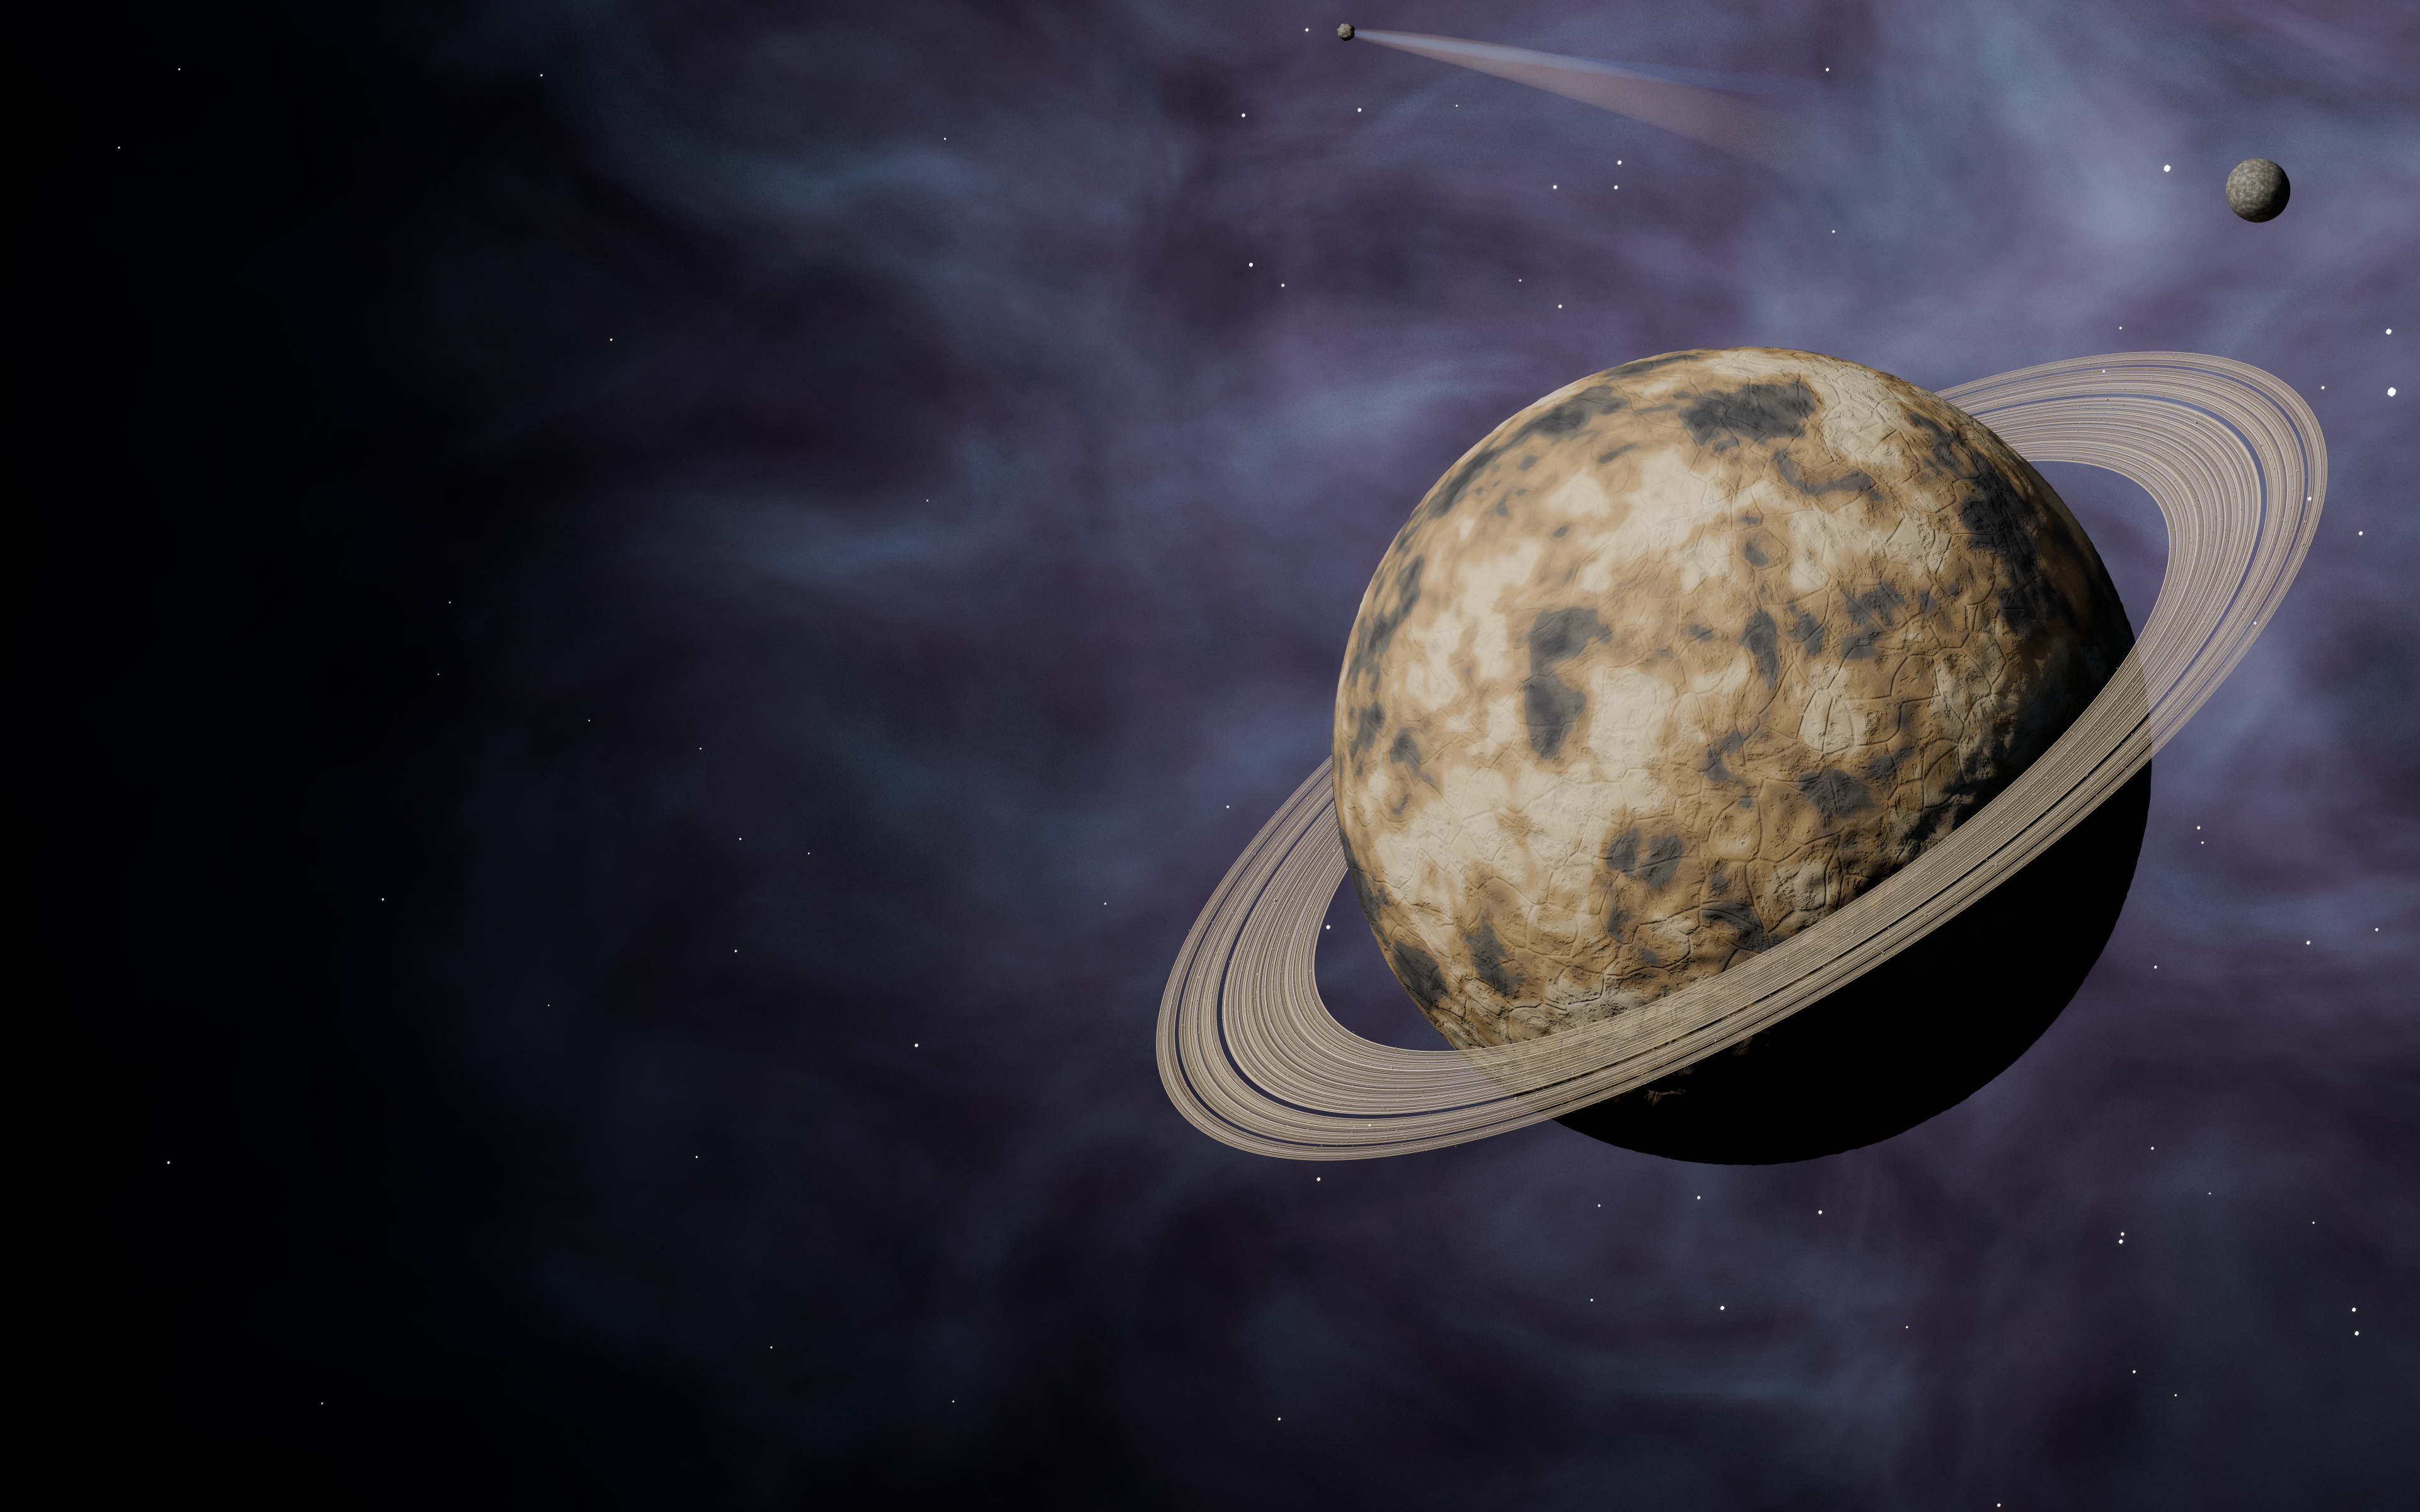
\includegraphics[width=20cm,height=12.5cm]{Risorse/Copertine/M07_Annula.jpg}};}{}
\node[anchor=north west,inner sep=0] at([xshift=1.05cm,yshift=-1.10cm]current page.north west){\color{Mint}\bfseries\fontsize{23}{28}\selectfont ANNULA};
\node[anchor=north west,inner sep=0] at([xshift=1.07cm,yshift=-2.16cm]current page.north west){\color{white}\fontsize{9}{12}\selectfont MODULO M07 · SCIENZE DELLA TERRA};
\draw[Mint,line width=1.5pt]([xshift=1.07cm,yshift=-2.78cm]current page.north west)--([xshift=2.6cm,yshift=-2.78cm]current page.north west);
\node[anchor=north west,inner sep=0] at([xshift=1.05cm,yshift=-3.35cm]current page.north west){\begin{minipage}{9.2cm}\raggedright\color{white}\bfseries\fontsize{30}{36}\selectfont Relazioni tra\\variabili e\\regressione\end{minipage}};
\node[anchor=north west,inner sep=0] at([xshift=1.07cm,yshift=-7.88cm]current page.north west){\begin{minipage}{8.9cm}\raggedright\color{Lilac}\fontsize{12.2}{17}\selectfont Stima, diagnostica\\e previsione in R\end{minipage}};
\node[anchor=north west,inner sep=0] at([xshift=1.07cm,yshift=-10.52cm]current page.north west){\color{white}\fontsize{11.5}{15}\selectfont Marzio De Corato};
\node[anchor=north west,inner sep=0] at([xshift=1.07cm,yshift=-11.17cm]current page.north west){\color{Mint}\fontsize{8.8}{11}\selectfont\href{https://creativecommons.org/licenses/by-nc-sa/4.0/}{© 2026 · CC BY-NC-SA 4.0}};
\end{tikzpicture}\end{frame}
\begin{frame}[plain]\hypertarget{slide2}{}
\bookmark[level=0,page=2]{Risposta e relazione}
\bookmark[level=1,page=2]{Una relazione descrive una risposta condizionata}
\begin{lrbox}{\PilotLeftBox}%
\begin{minipage}[t]{10.05cm}\raggedright\color{Ink}\fontsize{11.3}{14.8}\selectfont

\PLabel{Un fossile di diametro totale noto}
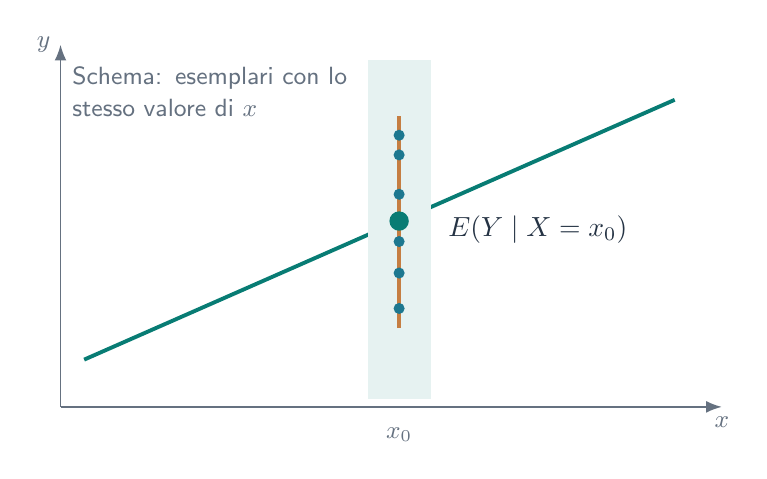
\begin{tikzpicture}[x=1cm,y=1cm]
\draw[pAxis](.7,.6)--(9.1,.6) node[pNote,below]{$x$};
\draw[pAxis](.7,.6)--(.7,5.2) node[pNote,left]{$y$};
\draw[Classical,line width=1.4pt](1,1.2)--(8.5,4.5);
\fill[Classical!10](4.6,.7) rectangle(5.4,5);
\draw[GeoB,line width=1.3pt](5,1.6)--(5,4.3);
\foreach \yy in {1.85,2.3,2.7,3.3,3.8,4.05}{\fill[GeoA](5,\yy) circle(2pt);}
\fill[Classical](5,2.96) circle(3.5pt);
\node[pLabel,anchor=west] at(5.5,2.85){$E(Y\mid X=x_0)$};
\node[pNote] at(5,.25){$x_0$};
\node[pNote,align=left,text width=3.5cm] at(2.6,4.6){Schema: esemplari con lo stesso valore di $x$};
\end{tikzpicture}

\end{minipage}%
\end{lrbox}
\typeout{FULLBOX:002:L:\the\ht\PilotLeftBox:\the\dp\PilotLeftBox}
\begin{lrbox}{\PilotRightBox}%
\begin{minipage}[t]{7.55cm}\raggedright\color{Ink}\fontsize{11.3}{14.8}\selectfont

\PBody{Il diametro totale aiuta a prevedere il diametro interno. A parità di diametro totale, i fossili conservano una variabilità.}
\vspace{4mm}
\[Y=m(X)+\varepsilon,\qquad E(\varepsilon\mid X)=0.\]
\PBody{La funzione $m(x)$ descrive la risposta media. L’errore $\varepsilon$ rappresenta gli scarti individuali attorno a quella media.}
\vspace{3mm}
\PInfo{La domanda scientifica precisa quali variabili sono disponibili quando occorre fare la previsione.}

\end{minipage}%
\end{lrbox}
\typeout{FULLBOX:002:R:\the\ht\PilotRightBox:\the\dp\PilotRightBox}
\begin{tikzpicture}[remember picture,overlay]
\PilotChrome{Una relazione descrive una risposta condizionata}{I · RISPOSTA E RELAZIONE}{2}{Il modello collega una risposta alle informazioni disponibili e conserva l’incertezza delle osservazioni.}
\node[anchor=north west,inner sep=0] at([xshift=0.96cm,yshift=-2.13cm]current page.north west){\usebox{\PilotLeftBox}};
\node[anchor=north west,inner sep=0] at([xshift=11.52cm,yshift=-2.13cm]current page.north west){\usebox{\PilotRightBox}};
\end{tikzpicture}\end{frame}

\begin{frame}[plain]\hypertarget{slide3}{}
\bookmark[level=1,page=3]{Risposta, predittore e unità di osservazione}
\begin{lrbox}{\PilotLeftBox}%
\begin{minipage}[t]{10.05cm}\raggedright\color{Ink}\fontsize{11.3}{14.8}\selectfont

\PLabel{La stessa tabella, una domanda precisa}
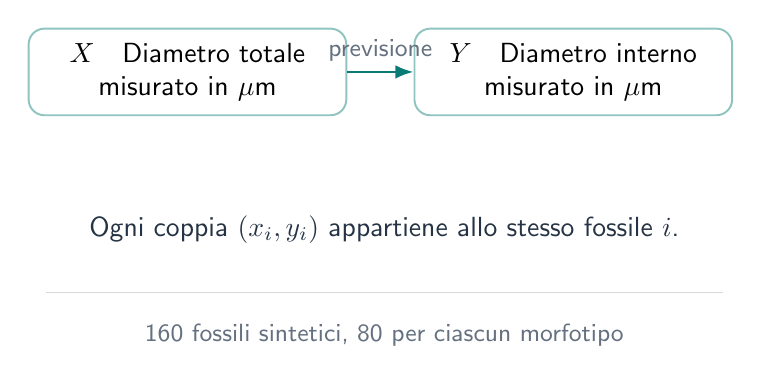
\begin{tikzpicture}[x=1cm,y=1cm]
\node[pFlow,text width=3.8cm] (x) at(2.3,3.6){$X$\quad Diametro totale\\misurato in $\mu$m};
\node[pFlow,text width=3.8cm] (y) at(7.2,3.6){$Y$\quad Diametro interno\\misurato in $\mu$m};
\draw[pEdge](x)--node[above,pNote]{previsione}(y);
\node[pLabel,text width=8.5cm] at(4.8,1.6){Ogni coppia $(x_i,y_i)$ appartiene allo stesso fossile $i$.};
\draw[Rule](.5,.8)--(9.1,.8);
\node[pNote,text width=8.5cm] at(4.8,.25){160 fossili sintetici, 80 per ciascun morfotipo};
\end{tikzpicture}
\PBody{Scambiare risposta e predittore cambia la domanda e il criterio di adattamento della regressione.}

\end{minipage}%
\end{lrbox}
\typeout{FULLBOX:003:L:\the\ht\PilotLeftBox:\the\dp\PilotLeftBox}
\begin{lrbox}{\PilotRightBox}%
\begin{minipage}[t]{7.55cm}\raggedright\color{Ink}\fontsize{11.3}{14.8}\selectfont

\PCode{R · leggere le coppie di misure}{003_dati.R}
\PSmall{Il file \texttt{setup.R} carica i dati in \texttt{f}. La sigla \texttt{um} nei nomi indica micrometri.}
\PInfo{Sono dati sintetici del corso. I risultati descrivono questo esempio didattico.}

\end{minipage}%
\end{lrbox}
\typeout{FULLBOX:003:R:\the\ht\PilotRightBox:\the\dp\PilotRightBox}
\begin{tikzpicture}[remember picture,overlay]
\PilotChrome{Risposta, predittore e unità di osservazione}{I · RISPOSTA E RELAZIONE}{3}{Prima della formula: un’unità di osservazione, una risposta, predittori disponibili e unità di misura.}
\node[anchor=north west,inner sep=0] at([xshift=0.96cm,yshift=-2.13cm]current page.north west){\usebox{\PilotLeftBox}};
\node[anchor=north west,inner sep=0] at([xshift=11.52cm,yshift=-2.13cm]current page.north west){\usebox{\PilotRightBox}};
\end{tikzpicture}\end{frame}

\begin{frame}[plain]\hypertarget{slide4}{}
\bookmark[level=1,page=4]{La geometria lega i due diametri}
\begin{lrbox}{\PilotLeftBox}%
\begin{minipage}[t]{10.05cm}\raggedright\color{Ink}\fontsize{11.3}{14.8}\selectfont

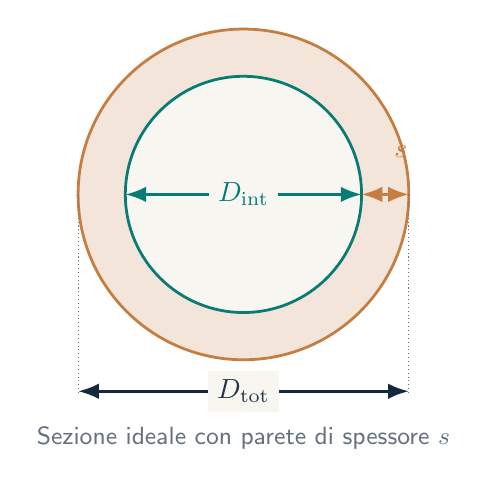
\begin{tikzpicture}[x=1cm,y=1cm]
\filldraw[fill=GeoB!20,draw=GeoB,line width=1pt](4.5,2.6) circle(2.1);
\filldraw[fill=Paper,draw=Classical,line width=1pt](4.5,2.6) circle(1.5);
\draw[Muted,densely dotted](2.4,2.6)--(2.4,.05);
\draw[Muted,densely dotted](6.6,2.6)--(6.6,.05);
\draw[{Latex}-{Latex},Navy,line width=1pt](2.4,.1)--(6.6,.1);
\node[pLabel,fill=Paper] at(4.5,.1){$D_{\rm tot}$};
\draw[{Latex}-{Latex},Classical,line width=1pt](3,2.6)--(6,2.6);
\node[pLabel,fill=Paper,text=Classical] at(4.5,2.6){$D_{\rm int}$};
\draw[{Latex}-{Latex},GeoB,line width=1pt](6,2.6)--(6.6,2.6);
\node[pLabel,text=GeoB] at(6.5,3.15){$s$};
\node[pNote] at(4.5,-.5){Sezione ideale con parete di spessore $s$};
\end{tikzpicture}
\PInfo{Ricostruire $D_{\rm int}$ da $D_{\rm tot}$ e $s$ applica l’identità geometrica: la domanda deve dichiararlo.}

\end{minipage}%
\end{lrbox}
\typeout{FULLBOX:004:L:\the\ht\PilotLeftBox:\the\dp\PilotLeftBox}
\begin{lrbox}{\PilotRightBox}%
\begin{minipage}[t]{7.55cm}\raggedright\color{Ink}\fontsize{11.3}{14.8}\selectfont

\[D_{\rm int}=D_{\rm tot}-2s.\]
\PCode{R · controllare l’identità}{004_geometria.R}
\PBody{Una parte dell’associazione nasce dalla definizione delle variabili. La dispersione dello spessore contribuisce alla dispersione del diametro interno.}

\end{minipage}%
\end{lrbox}
\typeout{FULLBOX:004:R:\the\ht\PilotRightBox:\the\dp\PilotRightBox}
\begin{tikzpicture}[remember picture,overlay]
\PilotChrome{La geometria lega i due diametri}{I · RISPOSTA E RELAZIONE}{4}{Una correlazione elevata può riflettere una definizione condivisa delle misure.}
\node[anchor=north west,inner sep=0] at([xshift=0.96cm,yshift=-2.13cm]current page.north west){\usebox{\PilotLeftBox}};
\node[anchor=north west,inner sep=0] at([xshift=11.52cm,yshift=-2.13cm]current page.north west){\usebox{\PilotRightBox}};
\end{tikzpicture}\end{frame}

\begin{frame}[plain]\hypertarget{slide5}{}
\bookmark[level=1,page=5]{La nuvola conserva le coppie di osservazioni}
\begin{lrbox}{\PilotLeftBox}%
\begin{minipage}[t]{10.05cm}\raggedright\color{Ink}\fontsize{11.3}{14.8}\selectfont
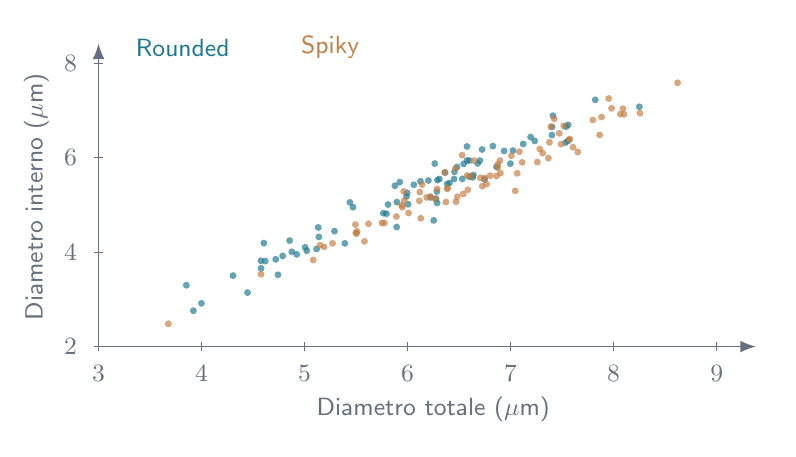
\begin{tikzpicture}[x=1cm,y=1cm]
\path[use as bounding box](-.25,-.4) rectangle(9.15,4.7);
\draw[pAxis](.65,.65)--(9,.65);
\draw[pAxis](.65,.65)--(.65,4.5);
\draw[Muted](0.6500,.59)--(0.6500,.71);\node[pNote] at(0.6500,.31){$ 3 $};
\draw[Muted](1.9583,.59)--(1.9583,.71);\node[pNote] at(1.9583,.31){$ 4 $};
\draw[Muted](3.2667,.59)--(3.2667,.71);\node[pNote] at(3.2667,.31){$ 5 $};
\draw[Muted](4.5750,.59)--(4.5750,.71);\node[pNote] at(4.5750,.31){$ 6 $};
\draw[Muted](5.8833,.59)--(5.8833,.71);\node[pNote] at(5.8833,.31){$ 7 $};
\draw[Muted](7.1917,.59)--(7.1917,.71);\node[pNote] at(7.1917,.31){$ 8 $};
\draw[Muted](8.5000,.59)--(8.5000,.71);\node[pNote] at(8.5000,.31){$ 9 $};
\draw[Muted](.59,0.6500)--(.71,0.6500);\node[pNote,anchor=east] at(.5,0.6500){$ 2 $};
\draw[Muted](.59,1.8500)--(.71,1.8500);\node[pNote,anchor=east] at(.5,1.8500){$ 4 $};
\draw[Muted](.59,3.0500)--(.71,3.0500);\node[pNote,anchor=east] at(.5,3.0500){$ 6 $};
\draw[Muted](.59,4.2500)--(.71,4.2500);\node[pNote,anchor=east] at(.5,4.2500){$ 8 $};
\node[pNote] at(4.9,-.15){Diametro totale ($\mu$m)};
\node[pNote,rotate=90] at(-.14,2.55){Diametro interno ($\mu$m)};
\fill[GeoA,opacity=.68](6.1897,3.2611) circle(1.25pt);
\fill[GeoA,opacity=.68](4.3267,2.4540) circle(1.25pt);
\fill[GeoA,opacity=.68](5.4096,2.8289) circle(1.25pt);
\fill[GeoA,opacity=.68](2.3576,1.5515) circle(1.25pt);
\fill[GeoA,opacity=.68](5.0513,2.8602) circle(1.25pt);
\fill[GeoA,opacity=.68](5.8011,3.1340) circle(1.25pt);
\fill[GeoA,opacity=.68](4.9498,2.4739) circle(1.25pt);
\fill[GeoA,opacity=.68](5.5533,2.7720) circle(1.25pt);
\fill[GeoA,opacity=.68](3.1051,1.8535) circle(1.25pt);
\fill[GeoA,opacity=.68](4.9363,2.5274) circle(1.25pt);
\fill[GeoA,opacity=.68](4.4363,2.1680) circle(1.25pt);
\fill[GeoA,opacity=.68](4.5694,2.6032) circle(1.25pt);
\fill[GeoA,opacity=.68](2.9003,1.7582) circle(1.25pt);
\fill[GeoA,opacity=.68](1.8549,1.1055) circle(1.25pt);
\fill[GeoA,opacity=.68](5.7031,2.9335) circle(1.25pt);
\fill[GeoA,opacity=.68](6.4093,3.4399) circle(1.25pt);
\fill[GeoA,opacity=.68](2.7501,1.9638) circle(1.25pt);
\fill[GeoA,opacity=.68](5.0777,2.7140) circle(1.25pt);
\fill[GeoA,opacity=.68](6.4083,3.3364) circle(1.25pt);
\fill[GeoA,opacity=.68](4.6548,2.7043) circle(1.25pt);
\fill[GeoA,opacity=.68](5.1658,2.7778) circle(1.25pt);
\fill[GeoA,opacity=.68](4.9778,2.7777) circle(1.25pt);
\fill[GeoA,opacity=.68](3.0769,1.9963) circle(1.25pt);
\fill[GeoA,opacity=.68](3.4405,2.1627) circle(1.25pt);
\fill[GeoA,opacity=.68](5.3290,3.0129) circle(1.25pt);
\fill[GeoA,opacity=.68](6.4214,3.5817) circle(1.25pt);
\fill[GeoA,opacity=.68](2.7120,1.7399) circle(1.25pt);
\fill[GeoA,opacity=.68](4.4141,2.6920) circle(1.25pt);
\fill[GeoA,opacity=.68](6.6143,3.4658) circle(1.25pt);
\fill[GeoA,opacity=.68](3.2947,1.8672) circle(1.25pt);
\fill[GeoA,opacity=.68](4.5810,2.4570) circle(1.25pt);
\fill[GeoA,opacity=.68](2.9884,1.8006) circle(1.25pt);
\fill[GeoA,opacity=.68](5.3587,3.0130) circle(1.25pt);
\fill[GeoA,opacity=.68](6.9579,3.7831) circle(1.25pt);
\fill[GeoA,opacity=.68](3.6469,2.1159) circle(1.25pt);
\fill[GeoA,opacity=.68](3.2736,1.9108) circle(1.25pt);
\fill[GeoA,opacity=.68](2.7672,1.7359) circle(1.25pt);
\fill[GeoA,opacity=.68](4.8663,2.5441) circle(1.25pt);
\fill[GeoA,opacity=.68](4.4756,2.7386) circle(1.25pt);
\fill[GeoA,opacity=.68](1.7650,1.4292) circle(1.25pt);
\fill[GeoA,opacity=.68](5.4928,3.0116) circle(1.25pt);
\fill[GeoA,opacity=.68](3.8415,2.4811) circle(1.25pt);
\fill[GeoA,opacity=.68](5.4655,2.9759) circle(1.25pt);
\fill[GeoA,opacity=.68](5.6580,3.1958) circle(1.25pt);
\fill[GeoA,opacity=.68](3.1668,1.8214) circle(1.25pt);
\fill[GeoA,opacity=.68](6.5804,3.2407) circle(1.25pt);
\fill[GeoA,opacity=.68](5.5215,3.1531) circle(1.25pt);
\fill[GeoA,opacity=.68](4.2664,2.3435) circle(1.25pt);
\fill[GeoA,opacity=.68](3.4480,2.0425) circle(1.25pt);
\fill[GeoA,opacity=.68](4.7386,2.7491) circle(1.25pt);
\fill[GeoA,opacity=.68](2.7137,1.6439) circle(1.25pt);
\fill[GeoA,opacity=.68](5.1706,2.8687) circle(1.25pt);
\fill[GeoA,opacity=.68](2.5419,1.3358) circle(1.25pt);
\fill[GeoA,opacity=.68](2.9290,1.5615) circle(1.25pt);
\fill[GeoA,opacity=.68](5.2026,2.9308) circle(1.25pt);
\fill[GeoA,opacity=.68](6.6109,3.2625) circle(1.25pt);
\fill[GeoA,opacity=.68](5.3589,2.8067) circle(1.25pt);
\fill[GeoA,opacity=.68](6.0434,3.2227) circle(1.25pt);
\fill[GeoA,opacity=.68](4.9067,2.2528) circle(1.25pt);
\fill[GeoA,opacity=.68](5.4016,2.7996) circle(1.25pt);
\fill[GeoA,opacity=.68](5.9133,3.1398) circle(1.25pt);
\fill[GeoA,opacity=.68](5.8798,2.9729) circle(1.25pt);
\fill[GeoA,opacity=.68](5.2871,2.9693) circle(1.25pt);
\fill[GeoA,opacity=.68](4.3058,2.3370) circle(1.25pt);
\fill[GeoA,opacity=.68](3.7786,1.9608) circle(1.25pt);
\fill[GeoA,opacity=.68](4.9535,2.7637) circle(1.25pt);
\fill[GeoA,opacity=.68](6.1374,3.3113) circle(1.25pt);
\fill[GeoA,opacity=.68](5.2695,2.7792) circle(1.25pt);
\fill[GeoA,opacity=.68](7.5178,3.6952) circle(1.25pt);
\fill[GeoA,opacity=.68](3.8817,2.4202) circle(1.25pt);
\fill[GeoA,opacity=.68](4.9197,2.9737) circle(1.25pt);
\fill[GeoA,opacity=.68](4.9469,2.6185) circle(1.25pt);
\fill[GeoA,opacity=.68](6.5873,3.4427) circle(1.25pt);
\fill[GeoA,opacity=.68](5.1065,2.7262) circle(1.25pt);
\fill[GeoA,opacity=.68](1.9571,1.1992) circle(1.25pt);
\fill[GeoA,opacity=.68](4.5615,2.5558) circle(1.25pt);
\fill[GeoA,opacity=.68](3.4190,1.8898) circle(1.25pt);
\fill[GeoA,opacity=.68](5.3289,3.1911) circle(1.25pt);
\fill[GeoA,opacity=.68](4.4386,2.4850) circle(1.25pt);
\fill[GeoA,opacity=.68](4.8386,2.7592) circle(1.25pt);
\fill[GeoB,opacity=.68](6.5006,3.3581) circle(1.25pt);
\fill[GeoB,opacity=.68](5.9671,2.8508) circle(1.25pt);
\fill[GeoB,opacity=.68](3.9187,2.0952) circle(1.25pt);
\fill[GeoB,opacity=.68](5.4185,3.0106) circle(1.25pt);
\fill[GeoB,opacity=.68](4.7241,2.5008) circle(1.25pt);
\fill[GeoB,opacity=.68](4.5318,2.5036) circle(1.25pt);
\fill[GeoB,opacity=.68](5.7043,2.8167) circle(1.25pt);
\fill[GeoB,opacity=.68](3.9125,2.1987) circle(1.25pt);
\fill[GeoB,opacity=.68](7.5265,3.6140) circle(1.25pt);
\fill[GeoB,opacity=.68](3.3767,1.7489) circle(1.25pt);
\fill[GeoB,opacity=.68](1.5369,0.9396) circle(1.25pt);
\fill[GeoB,opacity=.68](6.0301,2.9892) circle(1.25pt);
\fill[GeoB,opacity=.68](4.5873,2.3466) circle(1.25pt);
\fill[GeoB,opacity=.68](4.0787,2.2087) circle(1.25pt);
\fill[GeoB,opacity=.68](7.1656,3.6762) circle(1.25pt);
\fill[GeoB,opacity=.68](4.7584,2.7077) circle(1.25pt);
\fill[GeoB,opacity=.68](6.9273,3.5279) circle(1.25pt);
\fill[GeoB,opacity=.68](6.4365,3.5426) circle(1.25pt);
\fill[GeoB,opacity=.68](5.1891,2.4904) circle(1.25pt);
\fill[GeoB,opacity=.68](4.4335,2.3018) circle(1.25pt);
\fill[GeoB,opacity=.68](4.2498,2.2202) circle(1.25pt);
\fill[GeoB,opacity=.68](6.7371,3.1209) circle(1.25pt);
\fill[GeoB,opacity=.68](4.2805,2.2188) circle(1.25pt);
\fill[GeoB,opacity=.68](6.6270,3.2770) circle(1.25pt);
\fill[GeoB,opacity=.68](5.0825,2.6623) circle(1.25pt);
\fill[GeoB,opacity=.68](3.4635,1.9370) circle(1.25pt);
\fill[GeoB,opacity=.68](5.5779,2.7133) circle(1.25pt);
\fill[GeoB,opacity=.68](3.9263,2.0835) circle(1.25pt);
\fill[GeoB,opacity=.68](4.0271,1.9865) circle(1.25pt);
\fill[GeoB,opacity=.68](5.9945,3.1245) circle(1.25pt);
\fill[GeoB,opacity=.68](5.1824,2.9133) circle(1.25pt);
\fill[GeoB,opacity=.68](3.5151,1.9164) circle(1.25pt);
\fill[GeoB,opacity=.68](5.9418,2.6273) circle(1.25pt);
\fill[GeoB,opacity=.68](4.7301,2.6119) circle(1.25pt);
\fill[GeoB,opacity=.68](4.5091,2.4191) circle(1.25pt);
\fill[GeoB,opacity=.68](5.2670,3.0811) circle(1.25pt);
\fill[GeoB,opacity=.68](7.0385,3.5655) circle(1.25pt);
\fill[GeoB,opacity=.68](6.3949,3.4414) circle(1.25pt);
\fill[GeoB,opacity=.68](6.5240,3.2203) circle(1.25pt);
\fill[GeoB,opacity=.68](8.0041,3.9996) circle(1.25pt);
\fill[GeoB,opacity=.68](3.6224,1.9612) circle(1.25pt);
\fill[GeoB,opacity=.68](5.0465,2.8610) circle(1.25pt);
\fill[GeoB,opacity=.68](6.3766,3.2450) circle(1.25pt);
\fill[GeoB,opacity=.68](7.0138,3.3370) circle(1.25pt);
\fill[GeoB,opacity=.68](5.3403,2.6413) circle(1.25pt);
\fill[GeoB,opacity=.68](5.2813,2.5876) circle(1.25pt);
\fill[GeoB,opacity=.68](5.0621,2.4857) circle(1.25pt);
\fill[GeoB,opacity=.68](5.7532,2.8526) circle(1.25pt);
\fill[GeoB,opacity=.68](4.8650,2.5564) circle(1.25pt);
\fill[GeoB,opacity=.68](4.5255,2.6209) circle(1.25pt);
\fill[GeoB,opacity=.68](4.7418,2.2794) circle(1.25pt);
\fill[GeoB,opacity=.68](5.4990,2.7924) circle(1.25pt);
\fill[GeoB,opacity=.68](7.1289,3.8002) circle(1.25pt);
\fill[GeoB,opacity=.68](5.3809,2.8132) circle(1.25pt);
\fill[GeoB,opacity=.68](5.8926,3.0732) circle(1.25pt);
\fill[GeoB,opacity=.68](5.5543,2.7911) circle(1.25pt);
\fill[GeoB,opacity=.68](7.3231,3.6000) circle(1.25pt);
\fill[GeoB,opacity=.68](2.7132,1.5682) circle(1.25pt);
\fill[GeoB,opacity=.68](5.2061,2.5533) circle(1.25pt);
\fill[GeoB,opacity=.68](6.6354,3.2852) circle(1.25pt);
\fill[GeoB,opacity=.68](7.3104,3.6713) circle(1.25pt);
\fill[GeoB,opacity=.68](6.2228,2.9929) circle(1.25pt);
\fill[GeoB,opacity=.68](4.9225,2.5265) circle(1.25pt);
\fill[GeoB,opacity=.68](7.2759,3.6028) circle(1.25pt);
\fill[GeoB,opacity=.68](3.9329,2.1139) circle(1.25pt);
\fill[GeoB,opacity=.68](6.6764,3.1814) circle(1.25pt);
\fill[GeoB,opacity=.68](5.7479,3.0118) circle(1.25pt);
\fill[GeoB,opacity=.68](5.0785,2.6527) circle(1.25pt);
\fill[GeoB,opacity=.68](5.6238,2.8199) circle(1.25pt);
\fill[GeoB,opacity=.68](6.3630,3.0431) circle(1.25pt);
\fill[GeoB,opacity=.68](6.2904,3.1070) circle(1.25pt);
\fill[GeoB,opacity=.68](6.2532,3.1599) circle(1.25pt);
\fill[GeoB,opacity=.68](4.9496,2.6527) circle(1.25pt);
\fill[GeoB,opacity=.68](6.5581,3.4532) circle(1.25pt);
\fill[GeoB,opacity=.68](5.7199,2.9222) circle(1.25pt);
\fill[GeoB,opacity=.68](4.8170,2.5444) circle(1.25pt);
\fill[GeoB,opacity=.68](5.7225,2.9662) circle(1.25pt);
\fill[GeoB,opacity=.68](5.3315,2.8222) circle(1.25pt);
\fill[GeoB,opacity=.68](4.4990,2.4444) circle(1.25pt);
\fill[GeoB,opacity=.68](5.5239,2.6875) circle(1.25pt);
\node[pNote,text=GeoA,anchor=west] at(1.0,4.45){Rounded};\node[pNote,text=GeoB,anchor=west] at(3.1,4.45){Spiky};
\end{tikzpicture}
\PInfo{Una figura iniziale aiuta a riconoscere forma, dominio e osservazioni insolite prima di sintetizzare tutto con un coefficiente.}

\end{minipage}%
\end{lrbox}
\typeout{FULLBOX:005:L:\the\ht\PilotLeftBox:\the\dp\PilotLeftBox}
\begin{lrbox}{\PilotRightBox}%
\begin{minipage}[t]{7.55cm}\raggedright\color{Ink}\fontsize{11.3}{14.8}\selectfont

\PCode{R · rappresentare le due variabili}{005_nuvola.R}
\PBody{L’andamento è crescente. I colori mantengono visibile il morfotipo e permettono di cercare differenze a parità di diametro totale.}

\end{minipage}%
\end{lrbox}
\typeout{FULLBOX:005:R:\the\ht\PilotRightBox:\the\dp\PilotRightBox}
\begin{tikzpicture}[remember picture,overlay]
\PilotChrome{La nuvola conserva le coppie di osservazioni}{I · RISPOSTA E RELAZIONE}{5}{Ogni punto mantiene l’abbinamento tra le due misure dello stesso fossile.}
\node[anchor=north west,inner sep=0] at([xshift=0.96cm,yshift=-2.13cm]current page.north west){\usebox{\PilotLeftBox}};
\node[anchor=north west,inner sep=0] at([xshift=11.52cm,yshift=-2.13cm]current page.north west){\usebox{\PilotRightBox}};
\end{tikzpicture}\end{frame}

\begin{frame}[plain]\hypertarget{slide6}{}
\bookmark[level=1,page=6]{Media marginale e media condizionata}
\begin{lrbox}{\PilotLeftBox}%
\begin{minipage}[t]{10.05cm}\raggedright\color{Ink}\fontsize{11.3}{14.8}\selectfont

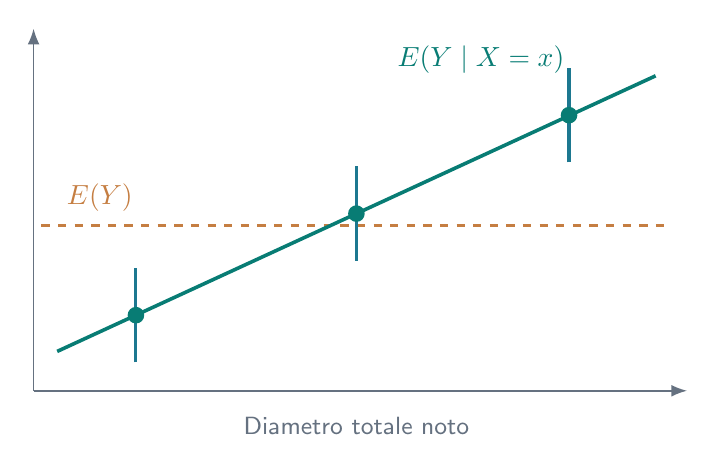
\begin{tikzpicture}[x=1cm,y=1cm]
\draw[pAxis](.7,.6)--(9,.6);\draw[pAxis](.7,.6)--(.7,5.2);
\draw[GeoB,dashed,line width=1.1pt](.8,2.7)--(8.7,2.7);
\draw[Classical,line width=1.3pt](1,1.1)--(8.6,4.6);
\foreach \xx/\yy in {2/1.56,4.8/2.85,7.5/4.1}{
\draw[GeoA,line width=1.1pt](\xx,\yy-.6)--(\xx,\yy+.6);
\fill[Classical](\xx,\yy) circle(3pt);}
\node[pLabel,anchor=west,text=GeoB] at(1,3.05){$E(Y)$};
\node[pLabel,anchor=west,text=Classical] at(5.2,4.8){$E(Y\mid X=x)$};
\node[pNote] at(4.8,.15){Diametro totale noto};
\end{tikzpicture}

\end{minipage}%
\end{lrbox}
\typeout{FULLBOX:006:L:\the\ht\PilotLeftBox:\the\dp\PilotLeftBox}
\begin{lrbox}{\PilotRightBox}%
\begin{minipage}[t]{7.55cm}\raggedright\color{Ink}\fontsize{11.3}{14.8}\selectfont

\PLabel{Quanto aiuta conoscere il predittore?}
\PBody{La media marginale assegna la stessa previsione a ogni fossile. La media condizionata cambia al variare del diametro totale.}
\[\hat y_{\rm base}=\bar y,\qquad \hat y(x)=\hat m(x).\]
\PBody{La variabilità residua riguarda esemplari confrontabili per $x$. Resta anche quando la retta descrive bene l’andamento medio.}

\end{minipage}%
\end{lrbox}
\typeout{FULLBOX:006:R:\the\ht\PilotRightBox:\the\dp\PilotRightBox}
\begin{tikzpicture}[remember picture,overlay]
\PilotChrome{Media marginale e media condizionata}{I · RISPOSTA E RELAZIONE}{6}{La regressione usa informazioni sul singolo caso per modificare la previsione della risposta.}
\node[anchor=north west,inner sep=0] at([xshift=0.96cm,yshift=-2.13cm]current page.north west){\usebox{\PilotLeftBox}};
\node[anchor=north west,inner sep=0] at([xshift=11.52cm,yshift=-2.13cm]current page.north west){\usebox{\PilotRightBox}};
\end{tikzpicture}\end{frame}

\begin{frame}[plain]\hypertarget{slide7}{}
\bookmark[level=1,page=7]{Il dominio osservato delimita l’esperienza}
\begin{lrbox}{\PilotLeftBox}%
\begin{minipage}[t]{10.05cm}\raggedright\color{Ink}\fontsize{11.3}{14.8}\selectfont

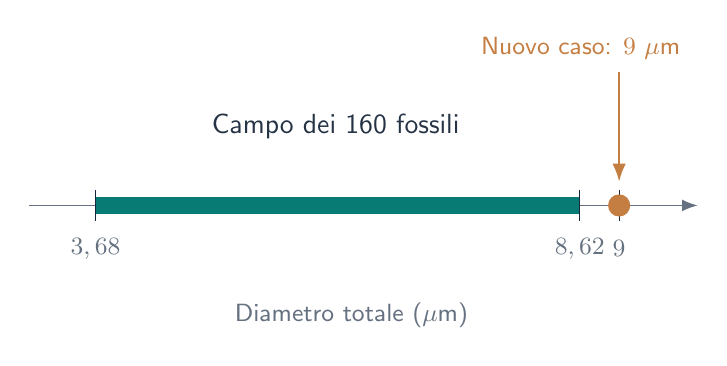
\begin{tikzpicture}[x=1cm,y=1cm]
\draw[pAxis](.7,2.1)--(9.2,2.1);
\draw[Classical,line width=6pt](1.55,2.1)--(7.7,2.1);
\foreach \x/\t in {1.55/{3,68},7.7/{8,62},8.2/9}{\draw[Navy](\x,1.9)--(\x,2.3);\node[pNote] at(\x,1.55){$\t$};}
\fill[GeoB](8.2,2.1) circle(4pt);
\node[pLabel] at(4.6,3.1){Campo dei 160 fossili};
\node[pNote,anchor=east,text=GeoB] at(9.1,4.1){Nuovo caso: $9\ \mu$m};
\draw[pEdge,GeoB](8.2,3.8)--(8.2,2.4);
\node[pNote] at(4.8,.7){Diametro totale ($\mu$m)};
\end{tikzpicture}

\end{minipage}%
\end{lrbox}
\typeout{FULLBOX:007:L:\the\ht\PilotLeftBox:\the\dp\PilotLeftBox}
\begin{lrbox}{\PilotRightBox}%
\begin{minipage}[t]{7.55cm}\raggedright\color{Ink}\fontsize{11.3}{14.8}\selectfont

\PCode{R · confrontare nuovo e osservato}{007_dominio.R}
\PBody{Il file copre circa $3{,}68$--$8{,}62\ \mu$m. Il valore $9\ \mu$m è già fuori dal campo osservato.}
\PLab{https://marzione00.github.io/Lab_Geo/\#laboratorio/m07-dominio}{Esperimento: dominio}
\PSmall{Nel sito la relazione vera è curva. Una retta stimata nel campo osservato può allontanarsi molto oltre quel campo.}

\end{minipage}%
\end{lrbox}
\typeout{FULLBOX:007:R:\the\ht\PilotRightBox:\the\dp\PilotRightBox}
\begin{tikzpicture}[remember picture,overlay]
\PilotChrome{Il dominio osservato delimita l’esperienza}{I · RISPOSTA E RELAZIONE}{7}{L’estrapolazione aggiunge un’ipotesi sulla validità del modello in condizioni non osservate.}
\node[anchor=north west,inner sep=0] at([xshift=0.96cm,yshift=-2.13cm]current page.north west){\usebox{\PilotLeftBox}};
\node[anchor=north west,inner sep=0] at([xshift=11.52cm,yshift=-2.13cm]current page.north west){\usebox{\PilotRightBox}};
\end{tikzpicture}\end{frame}

\begin{frame}[plain]\hypertarget{slide8}{}
\bookmark[level=1,page=8]{La correlazione riassume gli scarti concordi}
\begin{lrbox}{\PilotLeftBox}%
\begin{minipage}[t]{10.05cm}\raggedright\color{Ink}\fontsize{11.3}{14.8}\selectfont

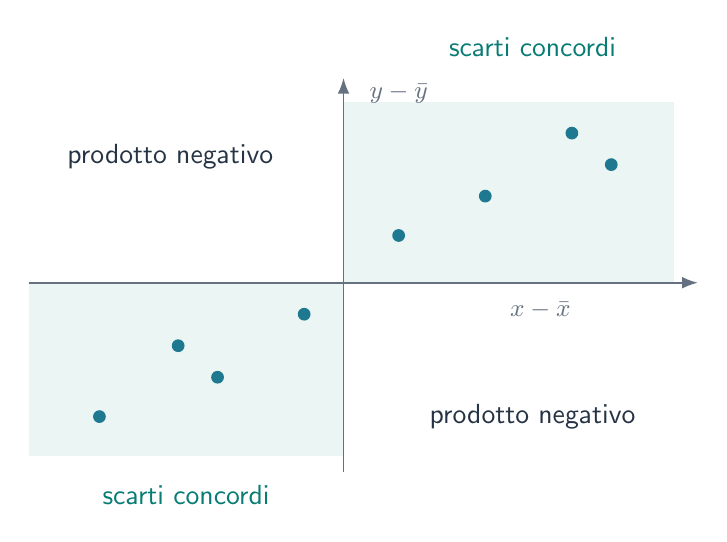
\begin{tikzpicture}[x=1cm,y=1cm]
\fill[Classical!8](.6,.6) rectangle(4.6,2.8);
\fill[Classical!8](4.6,2.8) rectangle(8.8,5.1);
\draw[pAxis](.6,2.8)--(9.1,2.8);\draw[pAxis](4.6,.4)--(4.6,5.4);
\foreach \x/\y in {1.5/1.1,2.5/2,3/1.6,4.1/2.4,5.3/3.4,6.4/3.9,7.5/4.7,8/4.3}{\fill[GeoA](\x,\y) circle(2.3pt);}
\node[pLabel] at(7,1.1){prodotto negativo};\node[pLabel] at(2.4,4.4){prodotto negativo};
\node[pLabel,text=Classical] at(2.6,.1){scarti concordi};\node[pLabel,text=Classical] at(7,5.8){scarti concordi};
\node[pNote] at(7.1,2.45){$x-\bar x$};\node[pNote] at(5.3,5.2){$y-\bar y$};
\end{tikzpicture}

\end{minipage}%
\end{lrbox}
\typeout{FULLBOX:008:L:\the\ht\PilotLeftBox:\the\dp\PilotLeftBox}
\begin{lrbox}{\PilotRightBox}%
\begin{minipage}[t]{7.55cm}\raggedright\color{Ink}\fontsize{11.3}{14.8}\selectfont

\[r=\frac{\sum_i(x_i-\bar x)(y_i-\bar y)}{\sqrt{\sum_i(x_i-\bar x)^2\sum_i(y_i-\bar y)^2}}.\]
\PBody{Gli scarti concordi danno contributi positivi. La normalizzazione elimina le unità e colloca $r$ tra $-1$ e $1$.}
\PInfo{Il coefficiente è definito quando entrambe le variabili hanno varianza positiva. Riassume l’associazione lineare.}

\end{minipage}%
\end{lrbox}
\typeout{FULLBOX:008:R:\the\ht\PilotRightBox:\the\dp\PilotRightBox}
\begin{tikzpicture}[remember picture,overlay]
\PilotChrome{La correlazione riassume gli scarti concordi}{I · RISPOSTA E RELAZIONE}{8}{Pearson confronta covariazione e dispersioni delle due variabili.}
\node[anchor=north west,inner sep=0] at([xshift=0.96cm,yshift=-2.13cm]current page.north west){\usebox{\PilotLeftBox}};
\node[anchor=north west,inner sep=0] at([xshift=11.52cm,yshift=-2.13cm]current page.north west){\usebox{\PilotRightBox}};
\end{tikzpicture}\end{frame}

\begin{frame}[plain]\hypertarget{slide9}{}
\bookmark[level=1,page=9]{Correlazione e unità di misura}
\begin{lrbox}{\PilotLeftBox}%
\begin{minipage}[t]{10.05cm}\raggedright\color{Ink}\fontsize{11.3}{14.8}\selectfont
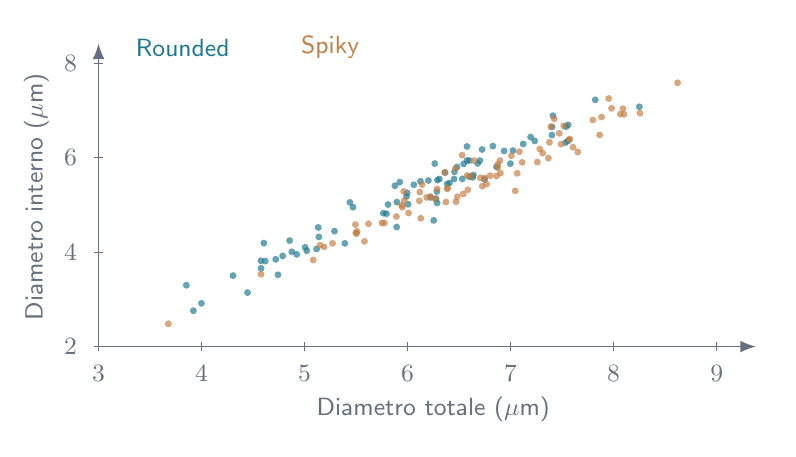
\begin{tikzpicture}[x=1cm,y=1cm]
\path[use as bounding box](-.25,-.4) rectangle(9.15,4.7);
\draw[pAxis](.65,.65)--(9,.65);
\draw[pAxis](.65,.65)--(.65,4.5);
\draw[Muted](0.6500,.59)--(0.6500,.71);\node[pNote] at(0.6500,.31){$ 3 $};
\draw[Muted](1.9583,.59)--(1.9583,.71);\node[pNote] at(1.9583,.31){$ 4 $};
\draw[Muted](3.2667,.59)--(3.2667,.71);\node[pNote] at(3.2667,.31){$ 5 $};
\draw[Muted](4.5750,.59)--(4.5750,.71);\node[pNote] at(4.5750,.31){$ 6 $};
\draw[Muted](5.8833,.59)--(5.8833,.71);\node[pNote] at(5.8833,.31){$ 7 $};
\draw[Muted](7.1917,.59)--(7.1917,.71);\node[pNote] at(7.1917,.31){$ 8 $};
\draw[Muted](8.5000,.59)--(8.5000,.71);\node[pNote] at(8.5000,.31){$ 9 $};
\draw[Muted](.59,0.6500)--(.71,0.6500);\node[pNote,anchor=east] at(.5,0.6500){$ 2 $};
\draw[Muted](.59,1.8500)--(.71,1.8500);\node[pNote,anchor=east] at(.5,1.8500){$ 4 $};
\draw[Muted](.59,3.0500)--(.71,3.0500);\node[pNote,anchor=east] at(.5,3.0500){$ 6 $};
\draw[Muted](.59,4.2500)--(.71,4.2500);\node[pNote,anchor=east] at(.5,4.2500){$ 8 $};
\node[pNote] at(4.9,-.15){Diametro totale ($\mu$m)};
\node[pNote,rotate=90] at(-.14,2.55){Diametro interno ($\mu$m)};
\fill[GeoA,opacity=.68](6.1897,3.2611) circle(1.25pt);
\fill[GeoA,opacity=.68](4.3267,2.4540) circle(1.25pt);
\fill[GeoA,opacity=.68](5.4096,2.8289) circle(1.25pt);
\fill[GeoA,opacity=.68](2.3576,1.5515) circle(1.25pt);
\fill[GeoA,opacity=.68](5.0513,2.8602) circle(1.25pt);
\fill[GeoA,opacity=.68](5.8011,3.1340) circle(1.25pt);
\fill[GeoA,opacity=.68](4.9498,2.4739) circle(1.25pt);
\fill[GeoA,opacity=.68](5.5533,2.7720) circle(1.25pt);
\fill[GeoA,opacity=.68](3.1051,1.8535) circle(1.25pt);
\fill[GeoA,opacity=.68](4.9363,2.5274) circle(1.25pt);
\fill[GeoA,opacity=.68](4.4363,2.1680) circle(1.25pt);
\fill[GeoA,opacity=.68](4.5694,2.6032) circle(1.25pt);
\fill[GeoA,opacity=.68](2.9003,1.7582) circle(1.25pt);
\fill[GeoA,opacity=.68](1.8549,1.1055) circle(1.25pt);
\fill[GeoA,opacity=.68](5.7031,2.9335) circle(1.25pt);
\fill[GeoA,opacity=.68](6.4093,3.4399) circle(1.25pt);
\fill[GeoA,opacity=.68](2.7501,1.9638) circle(1.25pt);
\fill[GeoA,opacity=.68](5.0777,2.7140) circle(1.25pt);
\fill[GeoA,opacity=.68](6.4083,3.3364) circle(1.25pt);
\fill[GeoA,opacity=.68](4.6548,2.7043) circle(1.25pt);
\fill[GeoA,opacity=.68](5.1658,2.7778) circle(1.25pt);
\fill[GeoA,opacity=.68](4.9778,2.7777) circle(1.25pt);
\fill[GeoA,opacity=.68](3.0769,1.9963) circle(1.25pt);
\fill[GeoA,opacity=.68](3.4405,2.1627) circle(1.25pt);
\fill[GeoA,opacity=.68](5.3290,3.0129) circle(1.25pt);
\fill[GeoA,opacity=.68](6.4214,3.5817) circle(1.25pt);
\fill[GeoA,opacity=.68](2.7120,1.7399) circle(1.25pt);
\fill[GeoA,opacity=.68](4.4141,2.6920) circle(1.25pt);
\fill[GeoA,opacity=.68](6.6143,3.4658) circle(1.25pt);
\fill[GeoA,opacity=.68](3.2947,1.8672) circle(1.25pt);
\fill[GeoA,opacity=.68](4.5810,2.4570) circle(1.25pt);
\fill[GeoA,opacity=.68](2.9884,1.8006) circle(1.25pt);
\fill[GeoA,opacity=.68](5.3587,3.0130) circle(1.25pt);
\fill[GeoA,opacity=.68](6.9579,3.7831) circle(1.25pt);
\fill[GeoA,opacity=.68](3.6469,2.1159) circle(1.25pt);
\fill[GeoA,opacity=.68](3.2736,1.9108) circle(1.25pt);
\fill[GeoA,opacity=.68](2.7672,1.7359) circle(1.25pt);
\fill[GeoA,opacity=.68](4.8663,2.5441) circle(1.25pt);
\fill[GeoA,opacity=.68](4.4756,2.7386) circle(1.25pt);
\fill[GeoA,opacity=.68](1.7650,1.4292) circle(1.25pt);
\fill[GeoA,opacity=.68](5.4928,3.0116) circle(1.25pt);
\fill[GeoA,opacity=.68](3.8415,2.4811) circle(1.25pt);
\fill[GeoA,opacity=.68](5.4655,2.9759) circle(1.25pt);
\fill[GeoA,opacity=.68](5.6580,3.1958) circle(1.25pt);
\fill[GeoA,opacity=.68](3.1668,1.8214) circle(1.25pt);
\fill[GeoA,opacity=.68](6.5804,3.2407) circle(1.25pt);
\fill[GeoA,opacity=.68](5.5215,3.1531) circle(1.25pt);
\fill[GeoA,opacity=.68](4.2664,2.3435) circle(1.25pt);
\fill[GeoA,opacity=.68](3.4480,2.0425) circle(1.25pt);
\fill[GeoA,opacity=.68](4.7386,2.7491) circle(1.25pt);
\fill[GeoA,opacity=.68](2.7137,1.6439) circle(1.25pt);
\fill[GeoA,opacity=.68](5.1706,2.8687) circle(1.25pt);
\fill[GeoA,opacity=.68](2.5419,1.3358) circle(1.25pt);
\fill[GeoA,opacity=.68](2.9290,1.5615) circle(1.25pt);
\fill[GeoA,opacity=.68](5.2026,2.9308) circle(1.25pt);
\fill[GeoA,opacity=.68](6.6109,3.2625) circle(1.25pt);
\fill[GeoA,opacity=.68](5.3589,2.8067) circle(1.25pt);
\fill[GeoA,opacity=.68](6.0434,3.2227) circle(1.25pt);
\fill[GeoA,opacity=.68](4.9067,2.2528) circle(1.25pt);
\fill[GeoA,opacity=.68](5.4016,2.7996) circle(1.25pt);
\fill[GeoA,opacity=.68](5.9133,3.1398) circle(1.25pt);
\fill[GeoA,opacity=.68](5.8798,2.9729) circle(1.25pt);
\fill[GeoA,opacity=.68](5.2871,2.9693) circle(1.25pt);
\fill[GeoA,opacity=.68](4.3058,2.3370) circle(1.25pt);
\fill[GeoA,opacity=.68](3.7786,1.9608) circle(1.25pt);
\fill[GeoA,opacity=.68](4.9535,2.7637) circle(1.25pt);
\fill[GeoA,opacity=.68](6.1374,3.3113) circle(1.25pt);
\fill[GeoA,opacity=.68](5.2695,2.7792) circle(1.25pt);
\fill[GeoA,opacity=.68](7.5178,3.6952) circle(1.25pt);
\fill[GeoA,opacity=.68](3.8817,2.4202) circle(1.25pt);
\fill[GeoA,opacity=.68](4.9197,2.9737) circle(1.25pt);
\fill[GeoA,opacity=.68](4.9469,2.6185) circle(1.25pt);
\fill[GeoA,opacity=.68](6.5873,3.4427) circle(1.25pt);
\fill[GeoA,opacity=.68](5.1065,2.7262) circle(1.25pt);
\fill[GeoA,opacity=.68](1.9571,1.1992) circle(1.25pt);
\fill[GeoA,opacity=.68](4.5615,2.5558) circle(1.25pt);
\fill[GeoA,opacity=.68](3.4190,1.8898) circle(1.25pt);
\fill[GeoA,opacity=.68](5.3289,3.1911) circle(1.25pt);
\fill[GeoA,opacity=.68](4.4386,2.4850) circle(1.25pt);
\fill[GeoA,opacity=.68](4.8386,2.7592) circle(1.25pt);
\fill[GeoB,opacity=.68](6.5006,3.3581) circle(1.25pt);
\fill[GeoB,opacity=.68](5.9671,2.8508) circle(1.25pt);
\fill[GeoB,opacity=.68](3.9187,2.0952) circle(1.25pt);
\fill[GeoB,opacity=.68](5.4185,3.0106) circle(1.25pt);
\fill[GeoB,opacity=.68](4.7241,2.5008) circle(1.25pt);
\fill[GeoB,opacity=.68](4.5318,2.5036) circle(1.25pt);
\fill[GeoB,opacity=.68](5.7043,2.8167) circle(1.25pt);
\fill[GeoB,opacity=.68](3.9125,2.1987) circle(1.25pt);
\fill[GeoB,opacity=.68](7.5265,3.6140) circle(1.25pt);
\fill[GeoB,opacity=.68](3.3767,1.7489) circle(1.25pt);
\fill[GeoB,opacity=.68](1.5369,0.9396) circle(1.25pt);
\fill[GeoB,opacity=.68](6.0301,2.9892) circle(1.25pt);
\fill[GeoB,opacity=.68](4.5873,2.3466) circle(1.25pt);
\fill[GeoB,opacity=.68](4.0787,2.2087) circle(1.25pt);
\fill[GeoB,opacity=.68](7.1656,3.6762) circle(1.25pt);
\fill[GeoB,opacity=.68](4.7584,2.7077) circle(1.25pt);
\fill[GeoB,opacity=.68](6.9273,3.5279) circle(1.25pt);
\fill[GeoB,opacity=.68](6.4365,3.5426) circle(1.25pt);
\fill[GeoB,opacity=.68](5.1891,2.4904) circle(1.25pt);
\fill[GeoB,opacity=.68](4.4335,2.3018) circle(1.25pt);
\fill[GeoB,opacity=.68](4.2498,2.2202) circle(1.25pt);
\fill[GeoB,opacity=.68](6.7371,3.1209) circle(1.25pt);
\fill[GeoB,opacity=.68](4.2805,2.2188) circle(1.25pt);
\fill[GeoB,opacity=.68](6.6270,3.2770) circle(1.25pt);
\fill[GeoB,opacity=.68](5.0825,2.6623) circle(1.25pt);
\fill[GeoB,opacity=.68](3.4635,1.9370) circle(1.25pt);
\fill[GeoB,opacity=.68](5.5779,2.7133) circle(1.25pt);
\fill[GeoB,opacity=.68](3.9263,2.0835) circle(1.25pt);
\fill[GeoB,opacity=.68](4.0271,1.9865) circle(1.25pt);
\fill[GeoB,opacity=.68](5.9945,3.1245) circle(1.25pt);
\fill[GeoB,opacity=.68](5.1824,2.9133) circle(1.25pt);
\fill[GeoB,opacity=.68](3.5151,1.9164) circle(1.25pt);
\fill[GeoB,opacity=.68](5.9418,2.6273) circle(1.25pt);
\fill[GeoB,opacity=.68](4.7301,2.6119) circle(1.25pt);
\fill[GeoB,opacity=.68](4.5091,2.4191) circle(1.25pt);
\fill[GeoB,opacity=.68](5.2670,3.0811) circle(1.25pt);
\fill[GeoB,opacity=.68](7.0385,3.5655) circle(1.25pt);
\fill[GeoB,opacity=.68](6.3949,3.4414) circle(1.25pt);
\fill[GeoB,opacity=.68](6.5240,3.2203) circle(1.25pt);
\fill[GeoB,opacity=.68](8.0041,3.9996) circle(1.25pt);
\fill[GeoB,opacity=.68](3.6224,1.9612) circle(1.25pt);
\fill[GeoB,opacity=.68](5.0465,2.8610) circle(1.25pt);
\fill[GeoB,opacity=.68](6.3766,3.2450) circle(1.25pt);
\fill[GeoB,opacity=.68](7.0138,3.3370) circle(1.25pt);
\fill[GeoB,opacity=.68](5.3403,2.6413) circle(1.25pt);
\fill[GeoB,opacity=.68](5.2813,2.5876) circle(1.25pt);
\fill[GeoB,opacity=.68](5.0621,2.4857) circle(1.25pt);
\fill[GeoB,opacity=.68](5.7532,2.8526) circle(1.25pt);
\fill[GeoB,opacity=.68](4.8650,2.5564) circle(1.25pt);
\fill[GeoB,opacity=.68](4.5255,2.6209) circle(1.25pt);
\fill[GeoB,opacity=.68](4.7418,2.2794) circle(1.25pt);
\fill[GeoB,opacity=.68](5.4990,2.7924) circle(1.25pt);
\fill[GeoB,opacity=.68](7.1289,3.8002) circle(1.25pt);
\fill[GeoB,opacity=.68](5.3809,2.8132) circle(1.25pt);
\fill[GeoB,opacity=.68](5.8926,3.0732) circle(1.25pt);
\fill[GeoB,opacity=.68](5.5543,2.7911) circle(1.25pt);
\fill[GeoB,opacity=.68](7.3231,3.6000) circle(1.25pt);
\fill[GeoB,opacity=.68](2.7132,1.5682) circle(1.25pt);
\fill[GeoB,opacity=.68](5.2061,2.5533) circle(1.25pt);
\fill[GeoB,opacity=.68](6.6354,3.2852) circle(1.25pt);
\fill[GeoB,opacity=.68](7.3104,3.6713) circle(1.25pt);
\fill[GeoB,opacity=.68](6.2228,2.9929) circle(1.25pt);
\fill[GeoB,opacity=.68](4.9225,2.5265) circle(1.25pt);
\fill[GeoB,opacity=.68](7.2759,3.6028) circle(1.25pt);
\fill[GeoB,opacity=.68](3.9329,2.1139) circle(1.25pt);
\fill[GeoB,opacity=.68](6.6764,3.1814) circle(1.25pt);
\fill[GeoB,opacity=.68](5.7479,3.0118) circle(1.25pt);
\fill[GeoB,opacity=.68](5.0785,2.6527) circle(1.25pt);
\fill[GeoB,opacity=.68](5.6238,2.8199) circle(1.25pt);
\fill[GeoB,opacity=.68](6.3630,3.0431) circle(1.25pt);
\fill[GeoB,opacity=.68](6.2904,3.1070) circle(1.25pt);
\fill[GeoB,opacity=.68](6.2532,3.1599) circle(1.25pt);
\fill[GeoB,opacity=.68](4.9496,2.6527) circle(1.25pt);
\fill[GeoB,opacity=.68](6.5581,3.4532) circle(1.25pt);
\fill[GeoB,opacity=.68](5.7199,2.9222) circle(1.25pt);
\fill[GeoB,opacity=.68](4.8170,2.5444) circle(1.25pt);
\fill[GeoB,opacity=.68](5.7225,2.9662) circle(1.25pt);
\fill[GeoB,opacity=.68](5.3315,2.8222) circle(1.25pt);
\fill[GeoB,opacity=.68](4.4990,2.4444) circle(1.25pt);
\fill[GeoB,opacity=.68](5.5239,2.6875) circle(1.25pt);
\node[pNote,text=GeoA,anchor=west] at(1.0,4.45){Rounded};\node[pNote,text=GeoB,anchor=west] at(3.1,4.45){Spiky};
\end{tikzpicture}
\PInfo{Pearson è simmetrico: $r(x,y)=r(y,x)$. La regressione assegna ruoli differenti a risposta e predittore.}

\end{minipage}%
\end{lrbox}
\typeout{FULLBOX:009:L:\the\ht\PilotLeftBox:\the\dp\PilotLeftBox}
\begin{lrbox}{\PilotRightBox}%
\begin{minipage}[t]{7.55cm}\raggedright\color{Ink}\fontsize{11.3}{14.8}\selectfont

\PCode{R · calcolare Pearson}{009_correlazione.R}
\[r=0{,}965\quad\text{nei 160 fossili}.\]
\PBody{Passare da micrometri a millimetri lascia invariata la correlazione. La pendenza conserva invece il rapporto fra le unità delle due variabili.}

\end{minipage}%
\end{lrbox}
\typeout{FULLBOX:009:R:\the\ht\PilotRightBox:\the\dp\PilotRightBox}
\begin{tikzpicture}[remember picture,overlay]
\PilotChrome{Correlazione e unità di misura}{I · RISPOSTA E RELAZIONE}{9}{Un numero senza unità misura associazione. Per prevedere la risposta serve anche la scala.}
\node[anchor=north west,inner sep=0] at([xshift=0.96cm,yshift=-2.13cm]current page.north west){\usebox{\PilotLeftBox}};
\node[anchor=north west,inner sep=0] at([xshift=11.52cm,yshift=-2.13cm]current page.north west){\usebox{\PilotRightBox}};
\end{tikzpicture}\end{frame}

\begin{frame}[plain]\hypertarget{slide10}{}
\bookmark[level=1,page=10]{Monotonia e linearità}
\begin{lrbox}{\PilotLeftBox}%
\begin{minipage}[t]{10.05cm}\raggedright\color{Ink}\fontsize{11.3}{14.8}\selectfont

\PLabel{Schema di una relazione crescente curva}
\begin{tikzpicture}[x=1cm,y=1cm]
\path[use as bounding box](-.25,-.4) rectangle(9.15,4.7);
\draw[pAxis](.65,.65)--(9,.65);
\draw[pAxis](.65,.65)--(.65,4.5);
\draw[Muted](0.6500,.59)--(0.6500,.71);\node[pNote] at(0.6500,.31){$ 0 $};
\draw[Muted](2.2200,.59)--(2.2200,.71);\node[pNote] at(2.2200,.31){$ 1 $};
\draw[Muted](3.7900,.59)--(3.7900,.71);\node[pNote] at(3.7900,.31){$ 2 $};
\draw[Muted](5.3600,.59)--(5.3600,.71);\node[pNote] at(5.3600,.31){$ 3 $};
\draw[Muted](6.9300,.59)--(6.9300,.71);\node[pNote] at(6.9300,.31){$ 4 $};
\draw[Muted](8.5000,.59)--(8.5000,.71);\node[pNote] at(8.5000,.31){$ 5 $};
\draw[Muted](.59,0.6500)--(.71,0.6500);\node[pNote,anchor=east] at(.5,0.6500){$ 0 $};
\draw[Muted](.59,1.6786)--(.71,1.6786);\node[pNote,anchor=east] at(.5,1.6786){$ 2 $};
\draw[Muted](.59,2.7071)--(.71,2.7071);\node[pNote,anchor=east] at(.5,2.7071){$ 4 $};
\draw[Muted](.59,3.7357)--(.71,3.7357);\node[pNote,anchor=east] at(.5,3.7357){$ 6 $};
\node[pNote] at(4.9,-.15){$x$};
\node[pNote,rotate=90] at(-.14,2.55){$y$};
\fill[GeoA](1.1210,0.7630) circle(1.7pt);
\fill[GeoA](1.4193,0.7800) circle(1.7pt);
\fill[GeoA](1.7176,0.8052) circle(1.7pt);
\fill[GeoA](2.0159,0.8385) circle(1.7pt);
\fill[GeoA](2.3142,0.8800) circle(1.7pt);
\fill[GeoA](2.6125,0.9296) circle(1.7pt);
\fill[GeoA](2.9108,0.9875) circle(1.7pt);
\fill[GeoA](3.2091,1.0535) circle(1.7pt);
\fill[GeoA](3.5074,1.1276) circle(1.7pt);
\fill[GeoA](3.8057,1.2100) circle(1.7pt);
\fill[GeoA](4.1040,1.3005) circle(1.7pt);
\fill[GeoA](4.4023,1.3991) circle(1.7pt);
\fill[GeoA](4.7006,1.5060) circle(1.7pt);
\fill[GeoA](4.9989,1.6210) circle(1.7pt);
\fill[GeoA](5.2972,1.7442) circle(1.7pt);
\fill[GeoA](5.5955,1.8755) circle(1.7pt);
\fill[GeoA](5.8938,2.0150) circle(1.7pt);
\fill[GeoA](6.1921,2.1627) circle(1.7pt);
\fill[GeoA](6.4904,2.3186) circle(1.7pt);
\fill[GeoA](6.7887,2.4826) circle(1.7pt);
\fill[GeoA](7.0870,2.6548) circle(1.7pt);
\fill[GeoA](7.3853,2.8351) circle(1.7pt);
\fill[GeoA](7.6836,3.0237) circle(1.7pt);
\fill[GeoA](7.9819,3.2204) circle(1.7pt);
\end{tikzpicture}
\PBody{Spearman riassume la concordanza degli ordinamenti. Una curva strettamente crescente può avere $r_S=1$ anche se la pendenza cambia con $x$.}

\end{minipage}%
\end{lrbox}
\typeout{FULLBOX:010:L:\the\ht\PilotLeftBox:\the\dp\PilotLeftBox}
\begin{lrbox}{\PilotRightBox}%
\begin{minipage}[t]{7.55cm}\raggedright\color{Ink}\fontsize{11.3}{14.8}\selectfont

\[r_S=\operatorname{cor}\{\operatorname{rank}(X),\operatorname{rank}(Y)\}.\]
\PCode{R · confrontare i ranghi}{010_ranghi.R}
\PSmall{Nei fossili: Pearson $0{,}965$, Spearman $0{,}952$. La figura resta necessaria per capire la forma.}

\end{minipage}%
\end{lrbox}
\typeout{FULLBOX:010:R:\the\ht\PilotRightBox:\the\dp\PilotRightBox}
\begin{tikzpicture}[remember picture,overlay]
\PilotChrome{Monotonia e linearità}{I · RISPOSTA E RELAZIONE}{10}{L’associazione monotona riguarda l’ordine. L’associazione lineare riguarda una retta.}
\node[anchor=north west,inner sep=0] at([xshift=0.96cm,yshift=-2.13cm]current page.north west){\usebox{\PilotLeftBox}};
\node[anchor=north west,inner sep=0] at([xshift=11.52cm,yshift=-2.13cm]current page.north west){\usebox{\PilotRightBox}};
\end{tikzpicture}\end{frame}

\begin{frame}[plain]\hypertarget{slide11}{}
\bookmark[level=1,page=11]{Una relazione curva può avere correlazione nulla}
\begin{lrbox}{\PilotLeftBox}%
\begin{minipage}[t]{10.05cm}\raggedright\color{Ink}\fontsize{11.3}{14.8}\selectfont
\begin{tikzpicture}[x=1cm,y=1cm]
\path[use as bounding box](-.25,-.4) rectangle(9.15,4.7);
\draw[pAxis](.65,.65)--(9,.65);
\draw[pAxis](.65,.65)--(.65,4.5);
\draw[Muted](0.6500,.59)--(0.6500,.71);\node[pNote] at(0.6500,.31){$ 0 $};
\draw[Muted](2.2200,.59)--(2.2200,.71);\node[pNote] at(2.2200,.31){$ 1 $};
\draw[Muted](3.7900,.59)--(3.7900,.71);\node[pNote] at(3.7900,.31){$ 2 $};
\draw[Muted](5.3600,.59)--(5.3600,.71);\node[pNote] at(5.3600,.31){$ 3 $};
\draw[Muted](6.9300,.59)--(6.9300,.71);\node[pNote] at(6.9300,.31){$ 4 $};
\draw[Muted](8.5000,.59)--(8.5000,.71);\node[pNote] at(8.5000,.31){$ 5 $};
\draw[Muted](.59,0.6500)--(.71,0.6500);\node[pNote,anchor=east] at(.5,0.6500){$ 0 $};
\draw[Muted](.59,1.6786)--(.71,1.6786);\node[pNote,anchor=east] at(.5,1.6786){$ 2 $};
\draw[Muted](.59,2.7071)--(.71,2.7071);\node[pNote,anchor=east] at(.5,2.7071){$ 4 $};
\draw[Muted](.59,3.7357)--(.71,3.7357);\node[pNote,anchor=east] at(.5,3.7357){$ 6 $};
\node[pNote] at(4.9,-.15){$x$};
\node[pNote,rotate=90] at(-.14,2.55){$y$};
\fill[GeoA](1.1210,2.9242) circle(1.7pt);
\fill[GeoA](1.4193,2.5951) circle(1.7pt);
\fill[GeoA](1.7176,2.2957) circle(1.7pt);
\fill[GeoA](2.0159,2.0260) circle(1.7pt);
\fill[GeoA](2.3142,1.7860) circle(1.7pt);
\fill[GeoA](2.6125,1.5757) circle(1.7pt);
\fill[GeoA](2.9108,1.3951) circle(1.7pt);
\fill[GeoA](3.2091,1.2443) circle(1.7pt);
\fill[GeoA](3.5074,1.1231) circle(1.7pt);
\fill[GeoA](3.8057,1.0316) circle(1.7pt);
\fill[GeoA](4.1040,0.9699) circle(1.7pt);
\fill[GeoA](4.4023,0.9378) circle(1.7pt);
\fill[GeoA](4.7006,0.9355) circle(1.7pt);
\fill[GeoA](4.9989,0.9629) circle(1.7pt);
\fill[GeoA](5.2972,1.0199) circle(1.7pt);
\fill[GeoA](5.5955,1.1067) circle(1.7pt);
\fill[GeoA](5.8938,1.2232) circle(1.7pt);
\fill[GeoA](6.1921,1.3693) circle(1.7pt);
\fill[GeoA](6.4904,1.5452) circle(1.7pt);
\fill[GeoA](6.7887,1.7508) circle(1.7pt);
\fill[GeoA](7.0870,1.9861) circle(1.7pt);
\fill[GeoA](7.3853,2.2511) circle(1.7pt);
\fill[GeoA](7.6836,2.5458) circle(1.7pt);
\fill[GeoA](7.9819,2.8702) circle(1.7pt);
\draw[GeoB,dashed,line width=1pt] plot coordinates {(0.6500,1.8329) (8.5000,1.8329)};
\end{tikzpicture}
\end{minipage}%
\end{lrbox}
\typeout{FULLBOX:011:L:\the\ht\PilotLeftBox:\the\dp\PilotLeftBox}
\begin{lrbox}{\PilotRightBox}%
\begin{minipage}[t]{7.55cm}\raggedright\color{Ink}\fontsize{11.3}{14.8}\selectfont

\[Y=X^2,\qquad X\sim U(-a,a).\]
\PBody{Per simmetria, $E(X)=E(X^3)=0$, quindi $\operatorname{Cov}(X,X^2)=0$. Eppure conoscere $X$ determina esattamente $Y$.}
\PCode{R · verificare un controesempio}{011_curvatura.R}
\PSmall{Il diagramma riproduce la forma a U su assi traslati e riscalati. La retta orizzontale ignora la sua struttura.}

\end{minipage}%
\end{lrbox}
\typeout{FULLBOX:011:R:\the\ht\PilotRightBox:\the\dp\PilotRightBox}
\begin{tikzpicture}[remember picture,overlay]
\PilotChrome{Una relazione curva può avere correlazione nulla}{I · RISPOSTA E RELAZIONE}{11}{Una correlazione vicina a zero esclude una forte associazione lineare, non ogni relazione.}
\node[anchor=north west,inner sep=0] at([xshift=0.96cm,yshift=-2.13cm]current page.north west){\usebox{\PilotLeftBox}};
\node[anchor=north west,inner sep=0] at([xshift=11.52cm,yshift=-2.13cm]current page.north west){\usebox{\PilotRightBox}};
\end{tikzpicture}\end{frame}

\begin{frame}[plain]\hypertarget{slide12}{}
\bookmark[level=1,page=12]{La restrizione del campo cambia la correlazione}
\begin{lrbox}{\PilotLeftBox}%
\begin{minipage}[t]{10.05cm}\raggedright\color{Ink}\fontsize{11.3}{14.8}\selectfont

\PLabel{Modello $Y=2X+\varepsilon$ con rumore invariato}
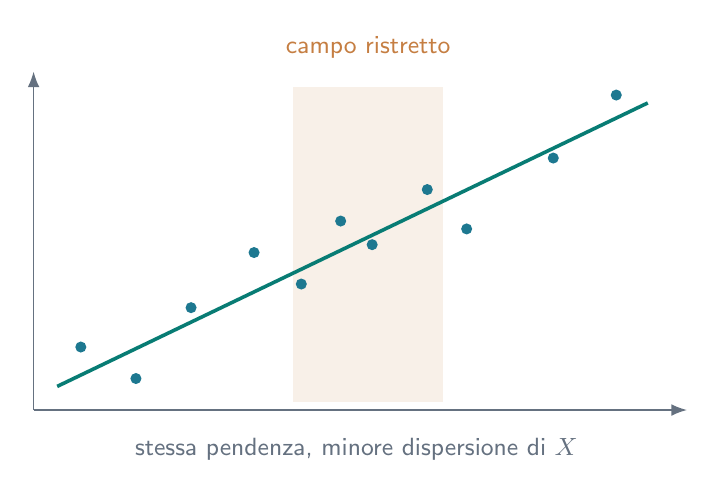
\begin{tikzpicture}[x=1cm,y=1cm]
\draw[pAxis](.7,.8)--(9,.8);\draw[pAxis](.7,.8)--(.7,5.1);
\fill[GeoB!12](4,.9) rectangle(5.9,4.9);
\draw[Classical,line width=1.3pt](1,1.1)--(8.5,4.7);
\foreach \x/\y in {1.3/1.6,2/1.2,2.7/2.1,3.5/2.8,4.1/2.4,4.6/3.2,5/2.9,5.7/3.6,6.2/3.1,7.3/4,8.1/4.8}{\fill[GeoA](\x,\y) circle(2pt);}
\node[pNote,text=GeoB] at(4.95,5.4){campo ristretto};
\node[pNote] at(4.8,.3){stessa pendenza, minore dispersione di $X$};
\end{tikzpicture}
\[\rho^2=\frac{\beta_1^2\operatorname{Var}(X)}{\beta_1^2\operatorname{Var}(X)+\sigma^2}.\]

\end{minipage}%
\end{lrbox}
\typeout{FULLBOX:012:L:\the\ht\PilotLeftBox:\the\dp\PilotLeftBox}
\begin{lrbox}{\PilotRightBox}%
\begin{minipage}[t]{7.55cm}\raggedright\color{Ink}\fontsize{11.3}{14.8}\selectfont

\PCode{R · restringere il campione}{012_campo.R}
\PLab{https://marzione00.github.io/Lab_Geo/\#laboratorio/m07-correlazione}{Esperimento: correlazione}
\PSmall{Con errore indipendente da $X$, la riduzione di $\operatorname{Var}(X)$ rende più grande il peso relativo del rumore.}

\end{minipage}%
\end{lrbox}
\typeout{FULLBOX:012:R:\the\ht\PilotRightBox:\the\dp\PilotRightBox}
\begin{tikzpicture}[remember picture,overlay]
\PilotChrome{La restrizione del campo cambia la correlazione}{I · RISPOSTA E RELAZIONE}{12}{La correlazione dipende anche dal campo dei predittori presente nel campione.}
\node[anchor=north west,inner sep=0] at([xshift=0.96cm,yshift=-2.13cm]current page.north west){\usebox{\PilotLeftBox}};
\node[anchor=north west,inner sep=0] at([xshift=11.52cm,yshift=-2.13cm]current page.north west){\usebox{\PilotRightBox}};
\end{tikzpicture}\end{frame}

\begin{frame}[plain]\hypertarget{slide13}{}
\bookmark[level=1,page=13]{Una causa comune può generare associazione}
\begin{lrbox}{\PilotLeftBox}%
\begin{minipage}[t]{10.05cm}\raggedright\color{Ink}\fontsize{11.3}{14.8}\selectfont

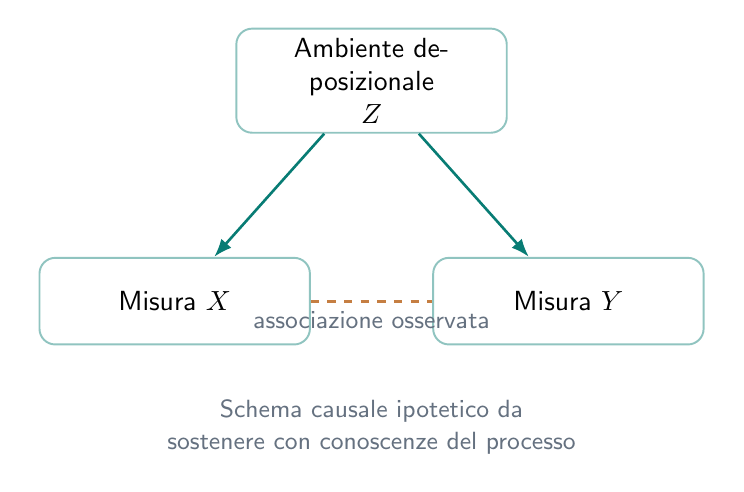
\begin{tikzpicture}[x=1cm,y=1cm]
\node[pFlow,text width=3.2cm] (z) at(4.8,4.8){Ambiente deposizionale\\$Z$};
\node[pFlow,text width=3.2cm] (x) at(2.3,2){Misura $X$};
\node[pFlow,text width=3.2cm] (y) at(7.3,2){Misura $Y$};
\draw[pEdge](z)--(x);\draw[pEdge](z)--(y);
\draw[GeoB,dashed,line width=1pt](x)--node[pNote,below]{associazione osservata}(y);
\node[pNote,text width=8.5cm] at(4.8,.4){Schema causale ipotetico da sostenere con conoscenze del processo};
\end{tikzpicture}

\end{minipage}%
\end{lrbox}
\typeout{FULLBOX:013:L:\the\ht\PilotLeftBox:\the\dp\PilotLeftBox}
\begin{lrbox}{\PilotRightBox}%
\begin{minipage}[t]{7.55cm}\raggedright\color{Ink}\fontsize{11.3}{14.8}\selectfont

\PBody{Una variabile comune può modificare entrambe le misure. Una relazione osservata tra $X$ e $Y$ può quindi dipendere dalla composizione del campione.}
\[E(Y\mid X=x)\quad\text{e}\quad E\{Y\mid \operatorname{do}(X=x)\}\]
\PSmall{La prima quantità è osservativa. La seconda descrive un intervento e richiede ipotesi causali aggiuntive. La notazione serve a distinguere le domande.}
\PInfo{Aggiungere variabili a una regressione richiede una ragione scientifica. La sola disponibilità di una colonna non basta.}

\end{minipage}%
\end{lrbox}
\typeout{FULLBOX:013:R:\the\ht\PilotRightBox:\the\dp\PilotRightBox}
\begin{tikzpicture}[remember picture,overlay]
\PilotChrome{Una causa comune può generare associazione}{I · RISPOSTA E RELAZIONE}{13}{La regressione descrive una relazione condizionata. Un’interpretazione causale richiede un disegno e ipotesi specifici.}
\node[anchor=north west,inner sep=0] at([xshift=0.96cm,yshift=-2.13cm]current page.north west){\usebox{\PilotLeftBox}};
\node[anchor=north west,inner sep=0] at([xshift=11.52cm,yshift=-2.13cm]current page.north west){\usebox{\PilotRightBox}};
\end{tikzpicture}\end{frame}

\begin{frame}[plain]\hypertarget{slide14}{}
\bookmark[level=0,page=14]{Modello lineare}
\bookmark[level=1,page=14]{Il modello lineare per la risposta media}
\begin{lrbox}{\PilotLeftBox}%
\begin{minipage}[t]{10.05cm}\raggedright\color{Ink}\fontsize{11.3}{14.8}\selectfont
\begin{tikzpicture}[x=1cm,y=1cm]
\path[use as bounding box](-.25,-.4) rectangle(9.15,4.7);
\draw[pAxis](.65,.65)--(9,.65);
\draw[pAxis](.65,.65)--(.65,4.5);
\draw[Muted](0.6500,.59)--(0.6500,.71);\node[pNote] at(0.6500,.31){$ 0 $};
\draw[Muted](2.2200,.59)--(2.2200,.71);\node[pNote] at(2.2200,.31){$ 1 $};
\draw[Muted](3.7900,.59)--(3.7900,.71);\node[pNote] at(3.7900,.31){$ 2 $};
\draw[Muted](5.3600,.59)--(5.3600,.71);\node[pNote] at(5.3600,.31){$ 3 $};
\draw[Muted](6.9300,.59)--(6.9300,.71);\node[pNote] at(6.9300,.31){$ 4 $};
\draw[Muted](8.5000,.59)--(8.5000,.71);\node[pNote] at(8.5000,.31){$ 5 $};
\draw[Muted](.59,0.6500)--(.71,0.6500);\node[pNote,anchor=east] at(.5,0.6500){$ 0 $};
\draw[Muted](.59,1.6786)--(.71,1.6786);\node[pNote,anchor=east] at(.5,1.6786){$ 2 $};
\draw[Muted](.59,2.7071)--(.71,2.7071);\node[pNote,anchor=east] at(.5,2.7071){$ 4 $};
\draw[Muted](.59,3.7357)--(.71,3.7357);\node[pNote,anchor=east] at(.5,3.7357){$ 6 $};
\node[pNote] at(4.9,-.15){$x$};
\node[pNote,rotate=90] at(-.14,2.55){$y$};
\fill[GeoA](1.1210,1.3031) circle(1.7pt);
\fill[GeoA](1.4193,1.6595) circle(1.7pt);
\fill[GeoA](1.7176,1.1213) circle(1.7pt);
\fill[GeoA](2.0159,1.7752) circle(1.7pt);
\fill[GeoA](2.3142,1.7352) circle(1.7pt);
\fill[GeoA](2.6125,1.4277) circle(1.7pt);
\fill[GeoA](2.9108,2.1705) circle(1.7pt);
\fill[GeoA](3.2091,1.7812) circle(1.7pt);
\fill[GeoA](3.5074,1.8502) circle(1.7pt);
\fill[GeoA](3.8057,2.4406) circle(1.7pt);
\fill[GeoA](4.1040,1.8779) circle(1.7pt);
\fill[GeoA](4.4023,2.3304) circle(1.7pt);
\fill[GeoA](4.7006,2.5832) circle(1.7pt);
\fill[GeoA](4.9989,2.0869) circle(1.7pt);
\fill[GeoA](5.2972,2.7886) circle(1.7pt);
\fill[GeoA](5.5955,2.6430) circle(1.7pt);
\fill[GeoA](5.8938,2.4284) circle(1.7pt);
\fill[GeoA](6.1921,3.1530) circle(1.7pt);
\fill[GeoA](6.4904,2.6951) circle(1.7pt);
\fill[GeoA](6.7887,2.8738) circle(1.7pt);
\fill[GeoA](7.0870,3.3866) circle(1.7pt);
\fill[GeoA](7.3853,2.8176) circle(1.7pt);
\fill[GeoA](7.6836,3.3561) circle(1.7pt);
\fill[GeoA](7.9819,3.5007) circle(1.7pt);
\draw[Classical,line width=1.1pt] plot coordinates {(0.6500,1.1643) (8.5000,3.4786)};
\end{tikzpicture}
\end{minipage}%
\end{lrbox}
\typeout{FULLBOX:014:L:\the\ht\PilotLeftBox:\the\dp\PilotLeftBox}
\begin{lrbox}{\PilotRightBox}%
\begin{minipage}[t]{7.55cm}\raggedright\color{Ink}\fontsize{11.3}{14.8}\selectfont

\[Y_i=\beta_0+\beta_1x_i+\varepsilon_i.\]
\PBody{Assumendo $E(\varepsilon_i\mid x_i)=0$, la risposta media condizionata è una retta:}
\[E(Y_i\mid x_i)=\beta_0+\beta_1x_i.\]
\PBody{I parametri $\beta_0$ e $\beta_1$ descrivono la popolazione nel modello. I dati producono le stime $\hat\beta_0$ e $\hat\beta_1$.}
\PInfo{Il diagramma è schematico. La scelta di una retta richiede un controllo della forma sui dati.}

\end{minipage}%
\end{lrbox}
\typeout{FULLBOX:014:R:\the\ht\PilotRightBox:\the\dp\PilotRightBox}
\begin{tikzpicture}[remember picture,overlay]
\PilotChrome{Il modello lineare per la risposta media}{II · MODELLO LINEARE}{14}{La linearità riguarda la media della risposta, non l’allineamento perfetto di tutti i punti.}
\node[anchor=north west,inner sep=0] at([xshift=0.96cm,yshift=-2.13cm]current page.north west){\usebox{\PilotLeftBox}};
\node[anchor=north west,inner sep=0] at([xshift=11.52cm,yshift=-2.13cm]current page.north west){\usebox{\PilotRightBox}};
\end{tikzpicture}\end{frame}

\begin{frame}[plain]\hypertarget{slide15}{}
\bookmark[level=1,page=15]{Intercetta e pendenza hanno un significato diverso}
\begin{lrbox}{\PilotLeftBox}%
\begin{minipage}[t]{10.05cm}\raggedright\color{Ink}\fontsize{11.3}{14.8}\selectfont

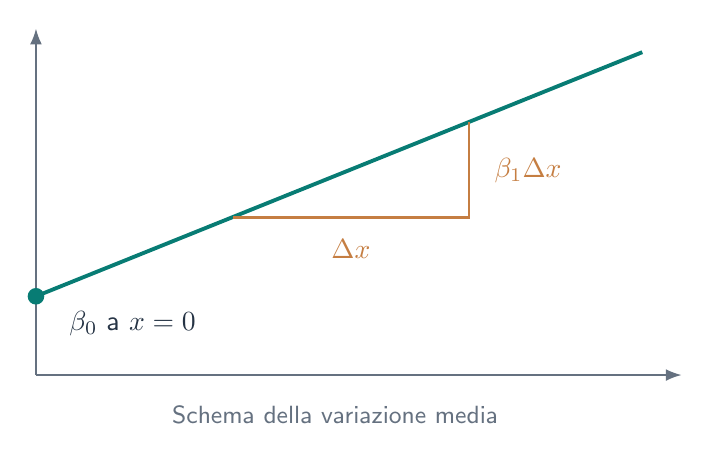
\begin{tikzpicture}[x=1cm,y=1cm]
\draw[pAxis](.8,.7)--(9,.7);\draw[pAxis](.8,.7)--(.8,5.1);
\draw[Classical,line width=1.4pt](.8,1.7)--(8.5,4.8);
\draw[GeoB,line width=1pt](3.3,2.7)--(6.3,2.7)--(6.3,3.91);
\node[pLabel,text=GeoB] at(4.8,2.3){$\Delta x$};
\node[pLabel,text=GeoB,anchor=west] at(6.5,3.3){$\beta_1\Delta x$};
\fill[Classical](.8,1.7) circle(3pt);
\node[pLabel,anchor=west] at(1.1,1.35){$\beta_0$ a $x=0$};
\node[pNote] at(4.6,.2){Schema della variazione media};
\end{tikzpicture}

\end{minipage}%
\end{lrbox}
\typeout{FULLBOX:015:L:\the\ht\PilotLeftBox:\the\dp\PilotLeftBox}
\begin{lrbox}{\PilotRightBox}%
\begin{minipage}[t]{7.55cm}\raggedright\color{Ink}\fontsize{11.3}{14.8}\selectfont

\[\beta_1=\frac{\Delta E(Y\mid x)}{\Delta x}.\]
\PBody{La pendenza indica quanto cambia la risposta media per un’unità in più del predittore. Ha unità $[Y]/[X]$.}
\vspace{3mm}
\PBody{L’intercetta è la media a $x=0$. La sua interpretazione fisica dipende dal dominio. Per i fossili, un diametro totale nullo è fuori dalle condizioni del campione.}

\end{minipage}%
\end{lrbox}
\typeout{FULLBOX:015:R:\the\ht\PilotRightBox:\the\dp\PilotRightBox}
\begin{tikzpicture}[remember picture,overlay]
\PilotChrome{Intercetta e pendenza hanno un significato diverso}{II · MODELLO LINEARE}{15}{Il valore algebrico dell’intercetta può essere utile al calcolo senza rappresentare un esemplare possibile.}
\node[anchor=north west,inner sep=0] at([xshift=0.96cm,yshift=-2.13cm]current page.north west){\usebox{\PilotLeftBox}};
\node[anchor=north west,inner sep=0] at([xshift=11.52cm,yshift=-2.13cm]current page.north west){\usebox{\PilotRightBox}};
\end{tikzpicture}\end{frame}

\begin{frame}[plain]\hypertarget{slide16}{}
\bookmark[level=1,page=16]{Errori del modello e residui osservabili}
\begin{lrbox}{\PilotLeftBox}%
\begin{minipage}[t]{10.05cm}\raggedright\color{Ink}\fontsize{11.3}{14.8}\selectfont

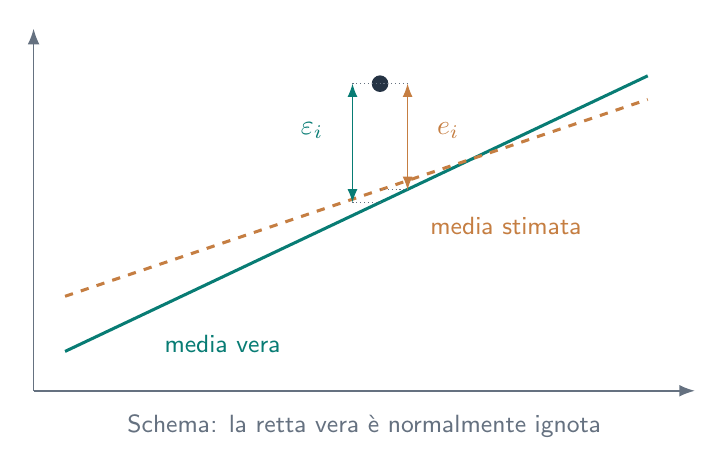
\begin{tikzpicture}[x=1cm,y=1cm]
\draw[pAxis](.6,.6)--(9,.6);\draw[pAxis](.6,.6)--(.6,5.2);
\draw[Classical,line width=1.1pt](1,1.1)--(8.4,4.6);
\draw[GeoB,dashed,line width=1.1pt](1,1.8)--(8.4,4.3);
\fill[Ink](5,4.5) circle(3pt);
\draw[Muted,densely dotted](4.65,4.5)--(5.35,4.5);
\draw[Muted,densely dotted](4.65,2.99189)--(5,2.99189);
\draw[Muted,densely dotted](5,3.15135)--(5.35,3.15135);
\draw[{Latex}-{Latex},Classical](4.65,2.99189)--(4.65,4.5);
\draw[{Latex}-{Latex},GeoB](5.35,3.15135)--(5.35,4.5);
\node[pLabel,text=Classical,anchor=east] at(4.4,3.9){$\varepsilon_i$};
\node[pLabel,text=GeoB,anchor=west] at(5.6,3.9){$e_i$};
\node[pNote,text=Classical] at(3.0,1.2){media vera};
\node[pNote,text=GeoB] at(6.6,2.7){media stimata};
\node[pNote] at(4.8,.15){Schema: la retta vera è normalmente ignota};
\end{tikzpicture}

\end{minipage}%
\end{lrbox}
\typeout{FULLBOX:016:L:\the\ht\PilotLeftBox:\the\dp\PilotLeftBox}
\begin{lrbox}{\PilotRightBox}%
\begin{minipage}[t]{7.55cm}\raggedright\color{Ink}\fontsize{11.3}{14.8}\selectfont

\[\varepsilon_i=y_i-E(Y_i\mid x_i),\qquad e_i=y_i-\hat y_i.\]
\PBody{Il residuo si calcola dopo la stima. L’errore rispetto alla media vera rimane generalmente ignoto.}
\PBody{Le ipotesi probabilistiche riguardano gli errori. I grafici dei residui permettono di cercare incompatibilità con quelle ipotesi.}
\PInfo{I residui di una regressione condividono i parametri stimati e non sono indipendenti tra loro.}

\end{minipage}%
\end{lrbox}
\typeout{FULLBOX:016:R:\the\ht\PilotRightBox:\the\dp\PilotRightBox}
\begin{tikzpicture}[remember picture,overlay]
\PilotChrome{Errori del modello e residui osservabili}{II · MODELLO LINEARE}{16}{Un residuo è una differenza calcolata rispetto a una funzione stimata dagli stessi dati.}
\node[anchor=north west,inner sep=0] at([xshift=0.96cm,yshift=-2.13cm]current page.north west){\usebox{\PilotLeftBox}};
\node[anchor=north west,inner sep=0] at([xshift=11.52cm,yshift=-2.13cm]current page.north west){\usebox{\PilotRightBox}};
\end{tikzpicture}\end{frame}

\begin{frame}[plain]\hypertarget{slide17}{}
\bookmark[level=1,page=17]{I minimi quadrati misurano scarti verticali}
\begin{lrbox}{\PilotLeftBox}%
\begin{minipage}[t]{10.05cm}\raggedright\color{Ink}\fontsize{11.3}{14.8}\selectfont
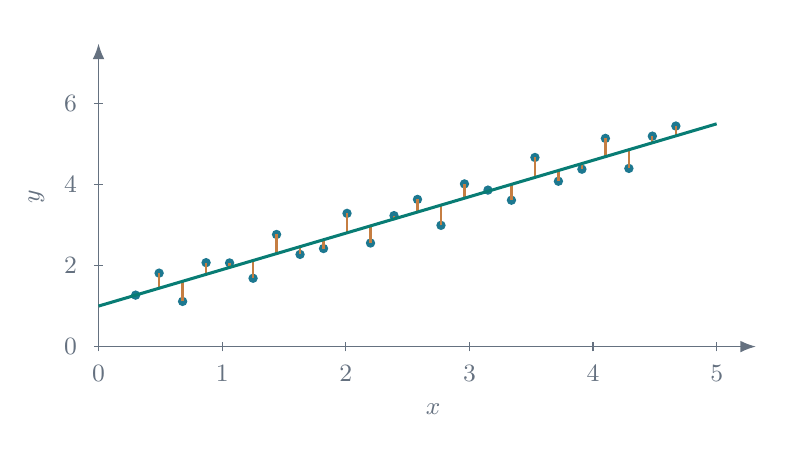
\begin{tikzpicture}[x=1cm,y=1cm]
\path[use as bounding box](-.25,-.4) rectangle(9.15,4.7);
\draw[pAxis](.65,.65)--(9,.65);
\draw[pAxis](.65,.65)--(.65,4.5);
\draw[Muted](0.6500,.59)--(0.6500,.71);\node[pNote] at(0.6500,.31){$ 0 $};
\draw[Muted](2.2200,.59)--(2.2200,.71);\node[pNote] at(2.2200,.31){$ 1 $};
\draw[Muted](3.7900,.59)--(3.7900,.71);\node[pNote] at(3.7900,.31){$ 2 $};
\draw[Muted](5.3600,.59)--(5.3600,.71);\node[pNote] at(5.3600,.31){$ 3 $};
\draw[Muted](6.9300,.59)--(6.9300,.71);\node[pNote] at(6.9300,.31){$ 4 $};
\draw[Muted](8.5000,.59)--(8.5000,.71);\node[pNote] at(8.5000,.31){$ 5 $};
\draw[Muted](.59,0.6500)--(.71,0.6500);\node[pNote,anchor=east] at(.5,0.6500){$ 0 $};
\draw[Muted](.59,1.6786)--(.71,1.6786);\node[pNote,anchor=east] at(.5,1.6786){$ 2 $};
\draw[Muted](.59,2.7071)--(.71,2.7071);\node[pNote,anchor=east] at(.5,2.7071){$ 4 $};
\draw[Muted](.59,3.7357)--(.71,3.7357);\node[pNote,anchor=east] at(.5,3.7357){$ 6 $};
\node[pNote] at(4.9,-.15){$x$};
\node[pNote,rotate=90] at(-.14,2.55){$y$};
\fill[GeoA](1.1210,1.3031) circle(1.7pt);
\draw[GeoB,line width=.8pt](1.1210,1.3031)--(1.1210,1.3031);
\fill[GeoA](1.4193,1.5828) circle(1.7pt);
\draw[GeoB,line width=.8pt](1.4193,1.5828)--(1.4193,1.3911);
\fill[GeoA](1.7176,1.2235) circle(1.7pt);
\draw[GeoB,line width=.8pt](1.7176,1.2235)--(1.7176,1.4790);
\fill[GeoA](2.0159,1.7157) circle(1.7pt);
\draw[GeoB,line width=.8pt](2.0159,1.7157)--(2.0159,1.5670);
\fill[GeoA](2.3142,1.7122) circle(1.7pt);
\draw[GeoB,line width=.8pt](2.3142,1.7122)--(2.3142,1.6549);
\fill[GeoA](2.6125,1.5177) circle(1.7pt);
\draw[GeoB,line width=.8pt](2.6125,1.5177)--(2.6125,1.7429);
\fill[GeoA](2.9108,2.0735) circle(1.7pt);
\draw[GeoB,line width=.8pt](2.9108,2.0735)--(2.9108,1.8308);
\fill[GeoA](3.2091,1.8205) circle(1.7pt);
\draw[GeoB,line width=.8pt](3.2091,1.8205)--(3.2091,1.9187);
\fill[GeoA](3.5074,1.8949) circle(1.7pt);
\draw[GeoB,line width=.8pt](3.5074,1.8949)--(3.5074,2.0067);
\fill[GeoA](3.8057,2.3418) circle(1.7pt);
\draw[GeoB,line width=.8pt](3.8057,2.3418)--(3.8057,2.0946);
\fill[GeoA](4.1040,1.9650) circle(1.7pt);
\draw[GeoB,line width=.8pt](4.1040,1.9650)--(4.1040,2.1826);
\fill[GeoA](4.4023,2.3133) circle(1.7pt);
\draw[GeoB,line width=.8pt](4.4023,2.3133)--(4.4023,2.2705);
\fill[GeoA](4.7006,2.5190) circle(1.7pt);
\draw[GeoB,line width=.8pt](4.7006,2.5190)--(4.7006,2.3585);
\fill[GeoA](4.9989,2.1896) circle(1.7pt);
\draw[GeoB,line width=.8pt](4.9989,2.1896)--(4.9989,2.4464);
\fill[GeoA](5.2972,2.7159) circle(1.7pt);
\draw[GeoB,line width=.8pt](5.2972,2.7159)--(5.2972,2.5343);
\fill[GeoA](5.5955,2.6371) circle(1.7pt);
\draw[GeoB,line width=.8pt](5.5955,2.6371)--(5.5955,2.6223);
\fill[GeoA](5.8938,2.5089) circle(1.7pt);
\draw[GeoB,line width=.8pt](5.8938,2.5089)--(5.8938,2.7102);
\fill[GeoA](6.1921,3.0516) circle(1.7pt);
\draw[GeoB,line width=.8pt](6.1921,3.0516)--(6.1921,2.7982);
\fill[GeoA](6.4904,2.7497) circle(1.7pt);
\draw[GeoB,line width=.8pt](6.4904,2.7497)--(6.4904,2.8861);
\fill[GeoA](6.7887,2.9024) circle(1.7pt);
\draw[GeoB,line width=.8pt](6.7887,2.9024)--(6.7887,2.9741);
\fill[GeoA](7.0870,3.2939) circle(1.7pt);
\draw[GeoB,line width=.8pt](7.0870,3.2939)--(7.0870,3.0620);
\fill[GeoA](7.3853,2.9126) circle(1.7pt);
\draw[GeoB,line width=.8pt](7.3853,2.9126)--(7.3853,3.1499);
\fill[GeoA](7.6836,3.3223) circle(1.7pt);
\draw[GeoB,line width=.8pt](7.6836,3.3223)--(7.6836,3.2379);
\fill[GeoA](7.9819,3.4507) circle(1.7pt);
\draw[GeoB,line width=.8pt](7.9819,3.4507)--(7.9819,3.3258);
\draw[Classical,line width=1.1pt] plot coordinates {(0.6500,1.1643) (8.5000,3.4786)};
\end{tikzpicture}
\PBody{Il criterio somma le distanze verticali al quadrato. Un grande scarto pesa più di diversi piccoli scarti della stessa somma assoluta.}
\PLab{https://marzione00.github.io/Lab_Geo/\#laboratorio/m07-minimi-quadrati}{Esperimento: minimi quadrati}

\end{minipage}%
\end{lrbox}
\typeout{FULLBOX:017:L:\the\ht\PilotLeftBox:\the\dp\PilotLeftBox}
\begin{lrbox}{\PilotRightBox}%
\begin{minipage}[t]{7.55cm}\raggedright\color{Ink}\fontsize{11.3}{14.8}\selectfont

\[S(b_0,b_1)=\sum_{i=1}^{n}\{y_i-(b_0+b_1x_i)\}^2.\]
\PCode{R · confrontare una retta proposta}{017_scarti.R}

\end{minipage}%
\end{lrbox}
\typeout{FULLBOX:017:R:\the\ht\PilotRightBox:\the\dp\PilotRightBox}
\begin{tikzpicture}[remember picture,overlay]
\PilotChrome{I minimi quadrati misurano scarti verticali}{II · MODELLO LINEARE}{17}{La regressione ordinaria minimizza gli scarti lungo l’asse della risposta.}
\node[anchor=north west,inner sep=0] at([xshift=0.96cm,yshift=-2.13cm]current page.north west){\usebox{\PilotLeftBox}};
\node[anchor=north west,inner sep=0] at([xshift=11.52cm,yshift=-2.13cm]current page.north west){\usebox{\PilotRightBox}};
\end{tikzpicture}\end{frame}

\begin{frame}[plain]\hypertarget{slide18}{}
\bookmark[level=1,page=18]{La somma dei quadrati ha un minimo}
\begin{lrbox}{\PilotLeftBox}%
\begin{minipage}[t]{10.05cm}\raggedright\color{Ink}\fontsize{11.3}{14.8}\selectfont

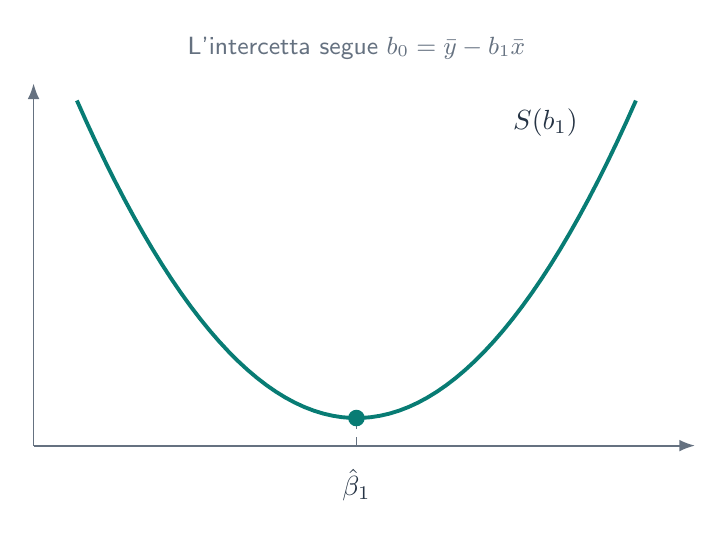
\begin{tikzpicture}[x=1cm,y=1cm]
\draw[pAxis](.7,.7)--(9.1,.7);\draw[pAxis](.7,.7)--(.7,5.3);
\draw[Classical,line width=1.4pt,domain=1.25:8.35,samples=60] plot(\x,{1.05+.32*(\x-4.8)^2});
\draw[Muted,dashed](4.8,.7)--(4.8,1.05);
\fill[Classical](4.8,1.05) circle(3pt);
\node[pLabel] at(4.8,.2){$\hat\beta_1$};
\node[pLabel] at(7.2,4.8){$S(b_1)$};
\node[pNote] at(4.8,5.75){L’intercetta segue $b_0=\bar y-b_1\bar x$};
\end{tikzpicture}

\end{minipage}%
\end{lrbox}
\typeout{FULLBOX:018:L:\the\ht\PilotLeftBox:\the\dp\PilotLeftBox}
\begin{lrbox}{\PilotRightBox}%
\begin{minipage}[t]{7.55cm}\raggedright\color{Ink}\fontsize{11.3}{14.8}\selectfont

\[S(b_1)=\sum_i\{(y_i-\bar y)-b_1(x_i-\bar x)\}^2.\]
\PBody{Dopo avere centrato le variabili, resta da scegliere una pendenza. Il criterio è una parabola convessa in $b_1$.}
\[\frac{\partial^2 S}{\partial b_1^2}=2\sum_i(x_i-\bar x)^2>0.\]
\PInfo{La disuguaglianza richiede almeno due valori diversi del predittore. In quel caso il minimo è unico.}

\end{minipage}%
\end{lrbox}
\typeout{FULLBOX:018:R:\the\ht\PilotRightBox:\the\dp\PilotRightBox}
\begin{tikzpicture}[remember picture,overlay]
\PilotChrome{La somma dei quadrati ha un minimo}{II · MODELLO LINEARE}{18}{La variabilità di X permette di identificare la pendenza.}
\node[anchor=north west,inner sep=0] at([xshift=0.96cm,yshift=-2.13cm]current page.north west){\usebox{\PilotLeftBox}};
\node[anchor=north west,inner sep=0] at([xshift=11.52cm,yshift=-2.13cm]current page.north west){\usebox{\PilotRightBox}};
\end{tikzpicture}\end{frame}

\begin{frame}[plain]\hypertarget{slide19}{}
\bookmark[level=1,page=19]{La prima equazione impone residui a somma zero}
\begin{lrbox}{\PilotLeftBox}%
\begin{minipage}[t]{10.05cm}\raggedright\color{Ink}\fontsize{11.3}{14.8}\selectfont

\PLabel{Derivata rispetto all’intercetta}
\[\frac{\partial S}{\partial b_0}=-2\sum_i(y_i-b_0-b_1x_i).\]
\[\sum_i y_i-n\hat\beta_0-\hat\beta_1\sum_i x_i=0.\]
\[\boxed{\hat\beta_0=\bar y-\hat\beta_1\bar x}\]
\PBody{La retta stimata attraversa il punto delle medie $(\bar x,\bar y)$. Il suo livello verticale si adatta alla media osservata.}

\end{minipage}%
\end{lrbox}
\typeout{FULLBOX:019:L:\the\ht\PilotLeftBox:\the\dp\PilotLeftBox}
\begin{lrbox}{\PilotRightBox}%
\begin{minipage}[t]{7.55cm}\raggedright\color{Ink}\fontsize{11.3}{14.8}\selectfont

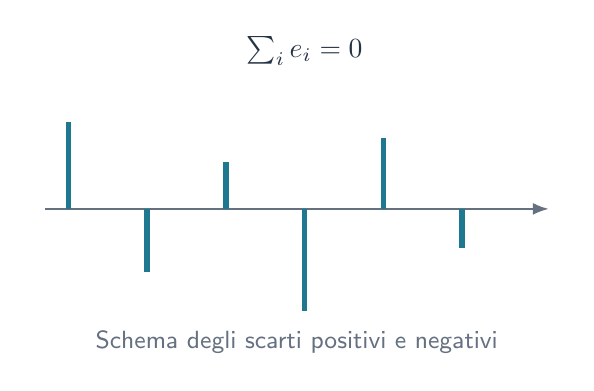
\begin{tikzpicture}[x=1cm,y=1cm]
\draw[pAxis](.5,2.7)--(6.9,2.7);
\foreach \x/\v in {.8/1.1,1.8/-.8,2.8/.6,3.8/-1.3,4.8/.9,5.8/-.5}{\draw[GeoA,line width=2pt](\x,2.7)--(\x,2.7+\v);}
\node[pLabel] at(3.8,4.7){$\sum_i e_i=0$};
\node[pNote,text width=6.6cm] at(3.7,1){Schema degli scarti positivi e negativi};
\end{tikzpicture}
\PInfo{La proprietà vale per minimi quadrati ordinari con intercetta. Non garantisce che il modello descriva bene la forma.}

\end{minipage}%
\end{lrbox}
\typeout{FULLBOX:019:R:\the\ht\PilotRightBox:\the\dp\PilotRightBox}
\begin{tikzpicture}[remember picture,overlay]
\PilotChrome{La prima equazione impone residui a somma zero}{II · MODELLO LINEARE}{19}{La somma zero dei residui è una conseguenza algebrica della stima con intercetta.}
\node[anchor=north west,inner sep=0] at([xshift=0.96cm,yshift=-2.13cm]current page.north west){\usebox{\PilotLeftBox}};
\node[anchor=north west,inner sep=0] at([xshift=11.52cm,yshift=-2.13cm]current page.north west){\usebox{\PilotRightBox}};
\end{tikzpicture}\end{frame}

\begin{frame}[plain]\hypertarget{slide20}{}
\bookmark[level=1,page=20]{La seconda equazione determina la pendenza}
\begin{lrbox}{\PilotLeftBox}%
\begin{minipage}[t]{10.05cm}\raggedright\color{Ink}\fontsize{11.3}{14.8}\selectfont

\PLabel{Derivata rispetto alla pendenza}
\[\frac{\partial S}{\partial b_1}=-2\sum_i x_i(y_i-b_0-b_1x_i).\]
\PBody{Sostituendo l’espressione dell’intercetta e raccogliendo gli scarti centrati:}
\[\sum_i(x_i-\bar x)(y_i-\bar y)=\hat\beta_1\sum_i(x_i-\bar x)^2.\]
\[\boxed{\hat\beta_1=\frac{S_{xy}}{S_{xx}}}\]

\end{minipage}%
\end{lrbox}
\typeout{FULLBOX:020:L:\the\ht\PilotLeftBox:\the\dp\PilotLeftBox}
\begin{lrbox}{\PilotRightBox}%
\begin{minipage}[t]{7.55cm}\raggedright\color{Ink}\fontsize{11.3}{14.8}\selectfont

\PLabel{Due quantità con ruoli diversi}
\[S_{xy}=\sum_i(x_i-\bar x)(y_i-\bar y),\]
\[S_{xx}=\sum_i(x_i-\bar x)^2.\]
\PBody{Il numeratore misura la covariazione. Il denominatore misura la dispersione del predittore.}
\PInfo{Se $S_{xx}=0$, tutti i valori di $x$ coincidono. I dati non separano intercetta e pendenza.}

\end{minipage}%
\end{lrbox}
\typeout{FULLBOX:020:R:\the\ht\PilotRightBox:\the\dp\PilotRightBox}
\begin{tikzpicture}[remember picture,overlay]
\PilotChrome{La seconda equazione determina la pendenza}{II · MODELLO LINEARE}{20}{La pendenza divide covariazione per dispersione del predittore.}
\node[anchor=north west,inner sep=0] at([xshift=0.96cm,yshift=-2.13cm]current page.north west){\usebox{\PilotLeftBox}};
\node[anchor=north west,inner sep=0] at([xshift=11.52cm,yshift=-2.13cm]current page.north west){\usebox{\PilotRightBox}};
\end{tikzpicture}\end{frame}

\begin{frame}[plain]\hypertarget{slide21}{}
\bookmark[level=1,page=21]{La retta attraversa il baricentro della nuvola}
\begin{lrbox}{\PilotLeftBox}%
\begin{minipage}[t]{10.05cm}\raggedright\color{Ink}\fontsize{11.3}{14.8}\selectfont
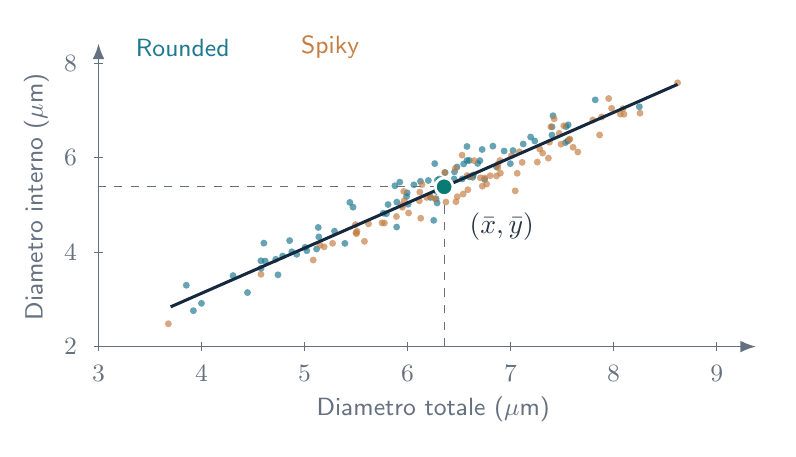
\begin{tikzpicture}[x=1cm,y=1cm]
\path[use as bounding box](-.25,-.4) rectangle(9.15,4.7);
\draw[pAxis](.65,.65)--(9,.65);
\draw[pAxis](.65,.65)--(.65,4.5);
\draw[Muted](0.6500,.59)--(0.6500,.71);\node[pNote] at(0.6500,.31){$ 3 $};
\draw[Muted](1.9583,.59)--(1.9583,.71);\node[pNote] at(1.9583,.31){$ 4 $};
\draw[Muted](3.2667,.59)--(3.2667,.71);\node[pNote] at(3.2667,.31){$ 5 $};
\draw[Muted](4.5750,.59)--(4.5750,.71);\node[pNote] at(4.5750,.31){$ 6 $};
\draw[Muted](5.8833,.59)--(5.8833,.71);\node[pNote] at(5.8833,.31){$ 7 $};
\draw[Muted](7.1917,.59)--(7.1917,.71);\node[pNote] at(7.1917,.31){$ 8 $};
\draw[Muted](8.5000,.59)--(8.5000,.71);\node[pNote] at(8.5000,.31){$ 9 $};
\draw[Muted](.59,0.6500)--(.71,0.6500);\node[pNote,anchor=east] at(.5,0.6500){$ 2 $};
\draw[Muted](.59,1.8500)--(.71,1.8500);\node[pNote,anchor=east] at(.5,1.8500){$ 4 $};
\draw[Muted](.59,3.0500)--(.71,3.0500);\node[pNote,anchor=east] at(.5,3.0500){$ 6 $};
\draw[Muted](.59,4.2500)--(.71,4.2500);\node[pNote,anchor=east] at(.5,4.2500){$ 8 $};
\node[pNote] at(4.9,-.15){Diametro totale ($\mu$m)};
\node[pNote,rotate=90] at(-.14,2.55){Diametro interno ($\mu$m)};
\fill[GeoA,opacity=.68](6.1897,3.2611) circle(1.25pt);
\fill[GeoA,opacity=.68](4.3267,2.4540) circle(1.25pt);
\fill[GeoA,opacity=.68](5.4096,2.8289) circle(1.25pt);
\fill[GeoA,opacity=.68](2.3576,1.5515) circle(1.25pt);
\fill[GeoA,opacity=.68](5.0513,2.8602) circle(1.25pt);
\fill[GeoA,opacity=.68](5.8011,3.1340) circle(1.25pt);
\fill[GeoA,opacity=.68](4.9498,2.4739) circle(1.25pt);
\fill[GeoA,opacity=.68](5.5533,2.7720) circle(1.25pt);
\fill[GeoA,opacity=.68](3.1051,1.8535) circle(1.25pt);
\fill[GeoA,opacity=.68](4.9363,2.5274) circle(1.25pt);
\fill[GeoA,opacity=.68](4.4363,2.1680) circle(1.25pt);
\fill[GeoA,opacity=.68](4.5694,2.6032) circle(1.25pt);
\fill[GeoA,opacity=.68](2.9003,1.7582) circle(1.25pt);
\fill[GeoA,opacity=.68](1.8549,1.1055) circle(1.25pt);
\fill[GeoA,opacity=.68](5.7031,2.9335) circle(1.25pt);
\fill[GeoA,opacity=.68](6.4093,3.4399) circle(1.25pt);
\fill[GeoA,opacity=.68](2.7501,1.9638) circle(1.25pt);
\fill[GeoA,opacity=.68](5.0777,2.7140) circle(1.25pt);
\fill[GeoA,opacity=.68](6.4083,3.3364) circle(1.25pt);
\fill[GeoA,opacity=.68](4.6548,2.7043) circle(1.25pt);
\fill[GeoA,opacity=.68](5.1658,2.7778) circle(1.25pt);
\fill[GeoA,opacity=.68](4.9778,2.7777) circle(1.25pt);
\fill[GeoA,opacity=.68](3.0769,1.9963) circle(1.25pt);
\fill[GeoA,opacity=.68](3.4405,2.1627) circle(1.25pt);
\fill[GeoA,opacity=.68](5.3290,3.0129) circle(1.25pt);
\fill[GeoA,opacity=.68](6.4214,3.5817) circle(1.25pt);
\fill[GeoA,opacity=.68](2.7120,1.7399) circle(1.25pt);
\fill[GeoA,opacity=.68](4.4141,2.6920) circle(1.25pt);
\fill[GeoA,opacity=.68](6.6143,3.4658) circle(1.25pt);
\fill[GeoA,opacity=.68](3.2947,1.8672) circle(1.25pt);
\fill[GeoA,opacity=.68](4.5810,2.4570) circle(1.25pt);
\fill[GeoA,opacity=.68](2.9884,1.8006) circle(1.25pt);
\fill[GeoA,opacity=.68](5.3587,3.0130) circle(1.25pt);
\fill[GeoA,opacity=.68](6.9579,3.7831) circle(1.25pt);
\fill[GeoA,opacity=.68](3.6469,2.1159) circle(1.25pt);
\fill[GeoA,opacity=.68](3.2736,1.9108) circle(1.25pt);
\fill[GeoA,opacity=.68](2.7672,1.7359) circle(1.25pt);
\fill[GeoA,opacity=.68](4.8663,2.5441) circle(1.25pt);
\fill[GeoA,opacity=.68](4.4756,2.7386) circle(1.25pt);
\fill[GeoA,opacity=.68](1.7650,1.4292) circle(1.25pt);
\fill[GeoA,opacity=.68](5.4928,3.0116) circle(1.25pt);
\fill[GeoA,opacity=.68](3.8415,2.4811) circle(1.25pt);
\fill[GeoA,opacity=.68](5.4655,2.9759) circle(1.25pt);
\fill[GeoA,opacity=.68](5.6580,3.1958) circle(1.25pt);
\fill[GeoA,opacity=.68](3.1668,1.8214) circle(1.25pt);
\fill[GeoA,opacity=.68](6.5804,3.2407) circle(1.25pt);
\fill[GeoA,opacity=.68](5.5215,3.1531) circle(1.25pt);
\fill[GeoA,opacity=.68](4.2664,2.3435) circle(1.25pt);
\fill[GeoA,opacity=.68](3.4480,2.0425) circle(1.25pt);
\fill[GeoA,opacity=.68](4.7386,2.7491) circle(1.25pt);
\fill[GeoA,opacity=.68](2.7137,1.6439) circle(1.25pt);
\fill[GeoA,opacity=.68](5.1706,2.8687) circle(1.25pt);
\fill[GeoA,opacity=.68](2.5419,1.3358) circle(1.25pt);
\fill[GeoA,opacity=.68](2.9290,1.5615) circle(1.25pt);
\fill[GeoA,opacity=.68](5.2026,2.9308) circle(1.25pt);
\fill[GeoA,opacity=.68](6.6109,3.2625) circle(1.25pt);
\fill[GeoA,opacity=.68](5.3589,2.8067) circle(1.25pt);
\fill[GeoA,opacity=.68](6.0434,3.2227) circle(1.25pt);
\fill[GeoA,opacity=.68](4.9067,2.2528) circle(1.25pt);
\fill[GeoA,opacity=.68](5.4016,2.7996) circle(1.25pt);
\fill[GeoA,opacity=.68](5.9133,3.1398) circle(1.25pt);
\fill[GeoA,opacity=.68](5.8798,2.9729) circle(1.25pt);
\fill[GeoA,opacity=.68](5.2871,2.9693) circle(1.25pt);
\fill[GeoA,opacity=.68](4.3058,2.3370) circle(1.25pt);
\fill[GeoA,opacity=.68](3.7786,1.9608) circle(1.25pt);
\fill[GeoA,opacity=.68](4.9535,2.7637) circle(1.25pt);
\fill[GeoA,opacity=.68](6.1374,3.3113) circle(1.25pt);
\fill[GeoA,opacity=.68](5.2695,2.7792) circle(1.25pt);
\fill[GeoA,opacity=.68](7.5178,3.6952) circle(1.25pt);
\fill[GeoA,opacity=.68](3.8817,2.4202) circle(1.25pt);
\fill[GeoA,opacity=.68](4.9197,2.9737) circle(1.25pt);
\fill[GeoA,opacity=.68](4.9469,2.6185) circle(1.25pt);
\fill[GeoA,opacity=.68](6.5873,3.4427) circle(1.25pt);
\fill[GeoA,opacity=.68](5.1065,2.7262) circle(1.25pt);
\fill[GeoA,opacity=.68](1.9571,1.1992) circle(1.25pt);
\fill[GeoA,opacity=.68](4.5615,2.5558) circle(1.25pt);
\fill[GeoA,opacity=.68](3.4190,1.8898) circle(1.25pt);
\fill[GeoA,opacity=.68](5.3289,3.1911) circle(1.25pt);
\fill[GeoA,opacity=.68](4.4386,2.4850) circle(1.25pt);
\fill[GeoA,opacity=.68](4.8386,2.7592) circle(1.25pt);
\fill[GeoB,opacity=.68](6.5006,3.3581) circle(1.25pt);
\fill[GeoB,opacity=.68](5.9671,2.8508) circle(1.25pt);
\fill[GeoB,opacity=.68](3.9187,2.0952) circle(1.25pt);
\fill[GeoB,opacity=.68](5.4185,3.0106) circle(1.25pt);
\fill[GeoB,opacity=.68](4.7241,2.5008) circle(1.25pt);
\fill[GeoB,opacity=.68](4.5318,2.5036) circle(1.25pt);
\fill[GeoB,opacity=.68](5.7043,2.8167) circle(1.25pt);
\fill[GeoB,opacity=.68](3.9125,2.1987) circle(1.25pt);
\fill[GeoB,opacity=.68](7.5265,3.6140) circle(1.25pt);
\fill[GeoB,opacity=.68](3.3767,1.7489) circle(1.25pt);
\fill[GeoB,opacity=.68](1.5369,0.9396) circle(1.25pt);
\fill[GeoB,opacity=.68](6.0301,2.9892) circle(1.25pt);
\fill[GeoB,opacity=.68](4.5873,2.3466) circle(1.25pt);
\fill[GeoB,opacity=.68](4.0787,2.2087) circle(1.25pt);
\fill[GeoB,opacity=.68](7.1656,3.6762) circle(1.25pt);
\fill[GeoB,opacity=.68](4.7584,2.7077) circle(1.25pt);
\fill[GeoB,opacity=.68](6.9273,3.5279) circle(1.25pt);
\fill[GeoB,opacity=.68](6.4365,3.5426) circle(1.25pt);
\fill[GeoB,opacity=.68](5.1891,2.4904) circle(1.25pt);
\fill[GeoB,opacity=.68](4.4335,2.3018) circle(1.25pt);
\fill[GeoB,opacity=.68](4.2498,2.2202) circle(1.25pt);
\fill[GeoB,opacity=.68](6.7371,3.1209) circle(1.25pt);
\fill[GeoB,opacity=.68](4.2805,2.2188) circle(1.25pt);
\fill[GeoB,opacity=.68](6.6270,3.2770) circle(1.25pt);
\fill[GeoB,opacity=.68](5.0825,2.6623) circle(1.25pt);
\fill[GeoB,opacity=.68](3.4635,1.9370) circle(1.25pt);
\fill[GeoB,opacity=.68](5.5779,2.7133) circle(1.25pt);
\fill[GeoB,opacity=.68](3.9263,2.0835) circle(1.25pt);
\fill[GeoB,opacity=.68](4.0271,1.9865) circle(1.25pt);
\fill[GeoB,opacity=.68](5.9945,3.1245) circle(1.25pt);
\fill[GeoB,opacity=.68](5.1824,2.9133) circle(1.25pt);
\fill[GeoB,opacity=.68](3.5151,1.9164) circle(1.25pt);
\fill[GeoB,opacity=.68](5.9418,2.6273) circle(1.25pt);
\fill[GeoB,opacity=.68](4.7301,2.6119) circle(1.25pt);
\fill[GeoB,opacity=.68](4.5091,2.4191) circle(1.25pt);
\fill[GeoB,opacity=.68](5.2670,3.0811) circle(1.25pt);
\fill[GeoB,opacity=.68](7.0385,3.5655) circle(1.25pt);
\fill[GeoB,opacity=.68](6.3949,3.4414) circle(1.25pt);
\fill[GeoB,opacity=.68](6.5240,3.2203) circle(1.25pt);
\fill[GeoB,opacity=.68](8.0041,3.9996) circle(1.25pt);
\fill[GeoB,opacity=.68](3.6224,1.9612) circle(1.25pt);
\fill[GeoB,opacity=.68](5.0465,2.8610) circle(1.25pt);
\fill[GeoB,opacity=.68](6.3766,3.2450) circle(1.25pt);
\fill[GeoB,opacity=.68](7.0138,3.3370) circle(1.25pt);
\fill[GeoB,opacity=.68](5.3403,2.6413) circle(1.25pt);
\fill[GeoB,opacity=.68](5.2813,2.5876) circle(1.25pt);
\fill[GeoB,opacity=.68](5.0621,2.4857) circle(1.25pt);
\fill[GeoB,opacity=.68](5.7532,2.8526) circle(1.25pt);
\fill[GeoB,opacity=.68](4.8650,2.5564) circle(1.25pt);
\fill[GeoB,opacity=.68](4.5255,2.6209) circle(1.25pt);
\fill[GeoB,opacity=.68](4.7418,2.2794) circle(1.25pt);
\fill[GeoB,opacity=.68](5.4990,2.7924) circle(1.25pt);
\fill[GeoB,opacity=.68](7.1289,3.8002) circle(1.25pt);
\fill[GeoB,opacity=.68](5.3809,2.8132) circle(1.25pt);
\fill[GeoB,opacity=.68](5.8926,3.0732) circle(1.25pt);
\fill[GeoB,opacity=.68](5.5543,2.7911) circle(1.25pt);
\fill[GeoB,opacity=.68](7.3231,3.6000) circle(1.25pt);
\fill[GeoB,opacity=.68](2.7132,1.5682) circle(1.25pt);
\fill[GeoB,opacity=.68](5.2061,2.5533) circle(1.25pt);
\fill[GeoB,opacity=.68](6.6354,3.2852) circle(1.25pt);
\fill[GeoB,opacity=.68](7.3104,3.6713) circle(1.25pt);
\fill[GeoB,opacity=.68](6.2228,2.9929) circle(1.25pt);
\fill[GeoB,opacity=.68](4.9225,2.5265) circle(1.25pt);
\fill[GeoB,opacity=.68](7.2759,3.6028) circle(1.25pt);
\fill[GeoB,opacity=.68](3.9329,2.1139) circle(1.25pt);
\fill[GeoB,opacity=.68](6.6764,3.1814) circle(1.25pt);
\fill[GeoB,opacity=.68](5.7479,3.0118) circle(1.25pt);
\fill[GeoB,opacity=.68](5.0785,2.6527) circle(1.25pt);
\fill[GeoB,opacity=.68](5.6238,2.8199) circle(1.25pt);
\fill[GeoB,opacity=.68](6.3630,3.0431) circle(1.25pt);
\fill[GeoB,opacity=.68](6.2904,3.1070) circle(1.25pt);
\fill[GeoB,opacity=.68](6.2532,3.1599) circle(1.25pt);
\fill[GeoB,opacity=.68](4.9496,2.6527) circle(1.25pt);
\fill[GeoB,opacity=.68](6.5581,3.4532) circle(1.25pt);
\fill[GeoB,opacity=.68](5.7199,2.9222) circle(1.25pt);
\fill[GeoB,opacity=.68](4.8170,2.5444) circle(1.25pt);
\fill[GeoB,opacity=.68](5.7225,2.9662) circle(1.25pt);
\fill[GeoB,opacity=.68](5.3315,2.8222) circle(1.25pt);
\fill[GeoB,opacity=.68](4.4990,2.4444) circle(1.25pt);
\fill[GeoB,opacity=.68](5.5239,2.6875) circle(1.25pt);
\draw[Navy,line width=1.1pt] plot coordinates {(1.5658,1.1544) (8.0028,3.9794)};
\draw[Muted,dashed](5.0390,.65)--(5.0390,2.6787)--(.65,2.6787);
\draw[white,line width=1pt,fill=Classical](5.0390,2.6787) circle(3.2pt);
\node[pLabel,anchor=north west] at(5.2390,2.4787){$ (\bar x,\bar y) $};
\node[pNote,text=GeoA,anchor=west] at(1.0,4.45){Rounded};\node[pNote,text=GeoB,anchor=west] at(3.1,4.45){Spiky};
\end{tikzpicture}
\end{minipage}%
\end{lrbox}
\typeout{FULLBOX:021:L:\the\ht\PilotLeftBox:\the\dp\PilotLeftBox}
\begin{lrbox}{\PilotRightBox}%
\begin{minipage}[t]{7.55cm}\raggedright\color{Ink}\fontsize{11.3}{14.8}\selectfont

\[\hat y=\bar y+\hat\beta_1(x-\bar x).\]
\PBody{Questa forma mette in evidenza il riferimento: la previsione parte dalla media della risposta e cambia secondo la distanza di $x$ dalla sua media.}
\[\bar x=6{,}355\ \mu\mathrm m,\qquad \bar y=5{,}381\ \mu\mathrm m.\]
\PInfo{La retta nella figura è stimata su tutti i 160 fossili per descrivere il campione. La valutazione predittiva userà un protocollo separato.}

\end{minipage}%
\end{lrbox}
\typeout{FULLBOX:021:R:\the\ht\PilotRightBox:\the\dp\PilotRightBox}
\begin{tikzpicture}[remember picture,overlay]
\PilotChrome{La retta attraversa il baricentro della nuvola}{II · MODELLO LINEARE}{21}{Centrare il predittore cambia l’intercetta, mentre pendenza e valori stimati restano uguali.}
\node[anchor=north west,inner sep=0] at([xshift=0.96cm,yshift=-2.13cm]current page.north west){\usebox{\PilotLeftBox}};
\node[anchor=north west,inner sep=0] at([xshift=11.52cm,yshift=-2.13cm]current page.north west){\usebox{\PilotRightBox}};
\end{tikzpicture}\end{frame}

\begin{frame}[plain]\hypertarget{slide22}{}
\bookmark[level=1,page=22]{La formula e il calcolo in R coincidono}
\begin{lrbox}{\PilotLeftBox}%
\begin{minipage}[t]{10.05cm}\raggedright\color{Ink}\fontsize{11.3}{14.8}\selectfont

\PLabel{Stime sui 160 fossili}
\[\hat\beta_0=-0{,}700282,\qquad\hat\beta_1=0{,}956997.\]
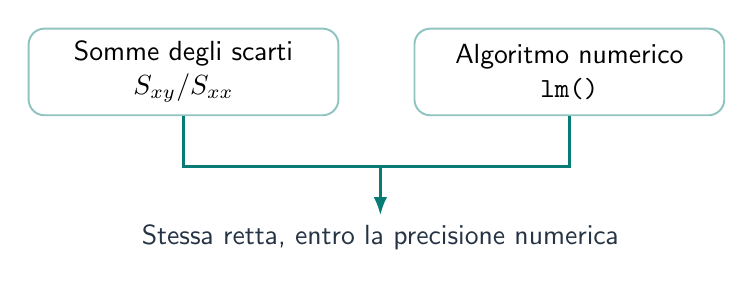
\begin{tikzpicture}[x=1cm,y=1cm]
\node[pFlow,text width=3.7cm] (a) at(2.3,3.3){Somme degli scarti\\$S_{xy}/S_{xx}$};
\node[pFlow,text width=3.7cm] (b) at(7.2,3.3){Algoritmo numerico\\\texttt{lm()}};
\node[pLabel] (stessa) at(4.8,1.2){Stessa retta, entro la precisione numerica};
\draw[Classical,line width=.95pt](a.south)--(2.3,2.1)--(7.2,2.1)--(b.south);
\draw[pEdge](4.8,2.1)--(stessa.north);
\end{tikzpicture}

\end{minipage}%
\end{lrbox}
\typeout{FULLBOX:022:L:\the\ht\PilotLeftBox:\the\dp\PilotLeftBox}
\begin{lrbox}{\PilotRightBox}%
\begin{minipage}[t]{7.55cm}\raggedright\color{Ink}\fontsize{11.3}{14.8}\selectfont

\PCode{R · ricostruire le stime}{022_minimi_mano.R}
\PSmall{\texttt{unname()} rimuove solo i nomi dei coefficienti. \texttt{all.equal()} confronta valori numerici con una tolleranza.}

\end{minipage}%
\end{lrbox}
\typeout{FULLBOX:022:R:\the\ht\PilotRightBox:\the\dp\PilotRightBox}
\begin{tikzpicture}[remember picture,overlay]
\PilotChrome{La formula e il calcolo in R coincidono}{II · MODELLO LINEARE}{22}{Ricostruire una stima semplice aiuta a capire che cosa calcola la funzione.}
\node[anchor=north west,inner sep=0] at([xshift=0.96cm,yshift=-2.13cm]current page.north west){\usebox{\PilotLeftBox}};
\node[anchor=north west,inner sep=0] at([xshift=11.52cm,yshift=-2.13cm]current page.north west){\usebox{\PilotRightBox}};
\end{tikzpicture}\end{frame}

\begin{frame}[plain]\hypertarget{slide23}{}
\bookmark[level=1,page=23]{La formula di R assegna i ruoli alle variabili}
\begin{lrbox}{\PilotLeftBox}%
\begin{minipage}[t]{10.05cm}\raggedright\color{Ink}\fontsize{11.3}{14.8}\selectfont

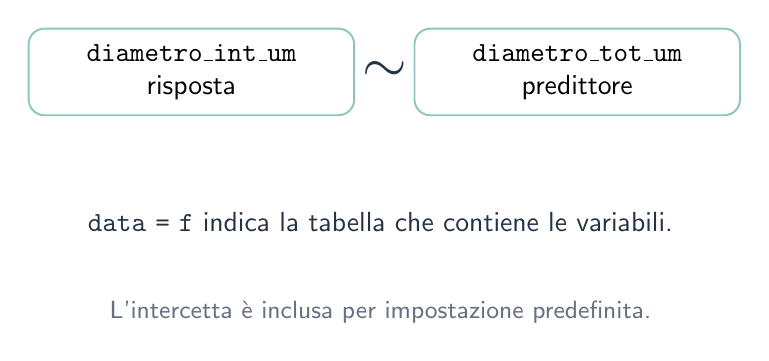
\begin{tikzpicture}[x=1cm,y=1cm]
\node[pFlow,text width=3.9cm] (a) at(2.4,3.7){\texttt{diametro\_int\_um}\\risposta};
\node[pFlow,text width=3.9cm] (b) at(7.3,3.7){\texttt{diametro\_tot\_um}\\predittore};
\node[pLabel,font=\fontsize{22}{25}\selectfont] at(4.85,3.7){$\sim$};
\node[pLabel,text width=8.4cm] at(4.8,1.8){\texttt{data = f} indica la tabella che contiene le variabili.};
\node[pNote,text width=8.4cm] at(4.8,.65){L’intercetta è inclusa per impostazione predefinita.};
\end{tikzpicture}

\end{minipage}%
\end{lrbox}
\typeout{FULLBOX:023:L:\the\ht\PilotLeftBox:\the\dp\PilotLeftBox}
\begin{lrbox}{\PilotRightBox}%
\begin{minipage}[t]{7.55cm}\raggedright\color{Ink}\fontsize{11.3}{14.8}\selectfont

\PCode{R · stimare e interrogare il modello}{023_lm.R}
\PSmall{\texttt{m0} conserva dati, formula e risultati. Le funzioni successive estraggono componenti specifiche senza ristimare manualmente il modello.}

\end{minipage}%
\end{lrbox}
\typeout{FULLBOX:023:R:\the\ht\PilotRightBox:\the\dp\PilotRightBox}
\begin{tikzpicture}[remember picture,overlay]
\PilotChrome{La formula di R assegna i ruoli alle variabili}{II · MODELLO LINEARE}{23}{Un oggetto lm conserva una procedura di stima e permette di interrogare risultati diversi.}
\node[anchor=north west,inner sep=0] at([xshift=0.96cm,yshift=-2.13cm]current page.north west){\usebox{\PilotLeftBox}};
\node[anchor=north west,inner sep=0] at([xshift=11.52cm,yshift=-2.13cm]current page.north west){\usebox{\PilotRightBox}};
\end{tikzpicture}\end{frame}

\begin{frame}[plain]\hypertarget{slide24}{}
\bookmark[level=1,page=24]{La pendenza traduce un incremento nelle unità}
\begin{lrbox}{\PilotLeftBox}%
\begin{minipage}[t]{10.05cm}\raggedright\color{Ink}\fontsize{11.3}{14.8}\selectfont

\PLabel{La retta stimata sui fossili}
\[\widehat D_{\rm int}=-0{,}700+0{,}957D_{\rm tot}.\]
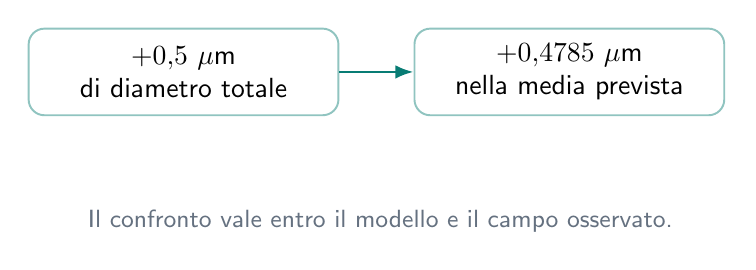
\begin{tikzpicture}[x=1cm,y=1cm]
\node[pFlow,text width=3.7cm] (a) at(2.3,2.9){$+0{,}5\ \mu$m\\di diametro totale};
\node[pFlow,text width=3.7cm] (b) at(7.2,2.9){$+0{,}4785\ \mu$m\\nella media prevista};
\draw[pEdge](a)--(b);
\node[pNote,text width=8.6cm] at(4.8,1){Il confronto vale entro il modello e il campo osservato.};
\end{tikzpicture}
\PInfo{Questa stima riassume l’associazione campionaria. Non quantifica l’effetto di modificare fisicamente un fossile.}

\end{minipage}%
\end{lrbox}
\typeout{FULLBOX:024:L:\the\ht\PilotLeftBox:\the\dp\PilotLeftBox}
\begin{lrbox}{\PilotRightBox}%
\begin{minipage}[t]{7.55cm}\raggedright\color{Ink}\fontsize{11.3}{14.8}\selectfont

\PCode{R · interpretare un incremento}{024_pendenza.R}
\PBody{Il coefficiente è circa $0{,}957\ \mu$m per $\mu$m. Le stesse unità al numeratore e denominatore si semplificano, ma l’interpretazione resta legata alle due misure.}

\end{minipage}%
\end{lrbox}
\typeout{FULLBOX:024:R:\the\ht\PilotRightBox:\the\dp\PilotRightBox}
\begin{tikzpicture}[remember picture,overlay]
\PilotChrome{La pendenza traduce un incremento nelle unità}{II · MODELLO LINEARE}{24}{Specificare incremento, unità e condizioni rende interpretabile un coefficiente.}
\node[anchor=north west,inner sep=0] at([xshift=0.96cm,yshift=-2.13cm]current page.north west){\usebox{\PilotLeftBox}};
\node[anchor=north west,inner sep=0] at([xshift=11.52cm,yshift=-2.13cm]current page.north west){\usebox{\PilotRightBox}};
\end{tikzpicture}\end{frame}

\begin{frame}[plain]\hypertarget{slide25}{}
\bookmark[level=1,page=25]{Le ipotesi sostengono conclusioni diverse}
\begin{lrbox}{\PilotLeftBox}%
\begin{minipage}[t]{10.05cm}\raggedright\color{Ink}\fontsize{11.3}{14.8}\selectfont

\PLabel{Dal calcolo all’inferenza}
\begin{tabular}{p{4.15cm}p{4.9cm}}
\toprule
\textbf{Condizione}&\textbf{Che cosa sostiene}\\\midrule
Matrice $X$ a rango pieno&Stima univoca dei coefficienti\\[2mm]
$E(\varepsilon\mid X)=0$&Non distorsione di OLS nel modello\\[2mm]
$\operatorname{Var}(\varepsilon\mid X)=\sigma^2I$&Formule classiche della varianza\\[2mm]
Normalità degli errori&Intervalli e test t esatti a campione finito\\\bottomrule
\end{tabular}

\end{minipage}%
\end{lrbox}
\typeout{FULLBOX:025:L:\the\ht\PilotLeftBox:\the\dp\PilotLeftBox}
\begin{lrbox}{\PilotRightBox}%
\begin{minipage}[t]{7.55cm}\raggedright\color{Ink}\fontsize{11.3}{14.8}\selectfont

\PBody{La retta dei minimi quadrati si può calcolare senza assumere normalità. Per interpretare l’incertezza occorre dichiarare ipotesi sulla generazione dei dati.}
\vspace{3mm}
\PBody{Indipendenza e campionamento coerente con la popolazione sono questioni del disegno. Un grafico dei residui può segnalare problemi, ma da solo non certifica il disegno.}
\PInfo{Nel seguito le formule classiche usano errori indipendenti, varianza costante e, per gli intervalli t esatti, normalità condizionata.}

\end{minipage}%
\end{lrbox}
\typeout{FULLBOX:025:R:\the\ht\PilotRightBox:\the\dp\PilotRightBox}
\begin{tikzpicture}[remember picture,overlay]
\PilotChrome{Le ipotesi sostengono conclusioni diverse}{II · MODELLO LINEARE}{25}{Una formula di stima e una formula d’incertezza possono richiedere condizioni differenti.}
\node[anchor=north west,inner sep=0] at([xshift=0.96cm,yshift=-2.13cm]current page.north west){\usebox{\PilotLeftBox}};
\node[anchor=north west,inner sep=0] at([xshift=11.52cm,yshift=-2.13cm]current page.north west){\usebox{\PilotRightBox}};
\end{tikzpicture}\end{frame}

\begin{frame}[plain]\hypertarget{slide26}{}
\bookmark[level=1,page=26]{La matrice del disegno raccoglie i predittori}
\begin{lrbox}{\PilotLeftBox}%
\begin{minipage}[t]{10.05cm}\raggedright\color{Ink}\fontsize{11.3}{14.8}\selectfont

\[\underbrace{\begin{pmatrix}y_1\\y_2\\\vdots\\y_n\end{pmatrix}}_{n\times1}
=\underbrace{\begin{pmatrix}1&x_1\\1&x_2\\\vdots&\vdots\\1&x_n\end{pmatrix}}_{X:\ n\times2}
\underbrace{\begin{pmatrix}\beta_0\\\beta_1\end{pmatrix}}_{2\times1}
+\underbrace{\begin{pmatrix}\varepsilon_1\\\varepsilon_2\\\vdots\\\varepsilon_n\end{pmatrix}}_{n\times1}.\]
\vspace{3mm}
\PBody{Ogni riga descrive un’osservazione. Ogni colonna rappresenta un termine della formula, compresa l’intercetta.}
\[\mathbf y=X\boldsymbol\beta+\boldsymbol\varepsilon.\]

\end{minipage}%
\end{lrbox}
\typeout{FULLBOX:026:L:\the\ht\PilotLeftBox:\the\dp\PilotLeftBox}
\begin{lrbox}{\PilotRightBox}%
\begin{minipage}[t]{7.55cm}\raggedright\color{Ink}\fontsize{11.3}{14.8}\selectfont

\PCode{R · vedere il disegno usato da lm}{026_matrice.R}
\PBody{Con $p$ coefficienti, $X$ ha $p$ colonne. Qui $p=2$. Nei modelli con gruppi, interazioni e trasformazioni sarà importante contare i coefficienti effettivi.}
\PInfo{Useremo $p$ includendo l’intercetta. I gradi di libertà residui sono $n-p$ se il rango è pieno.}

\end{minipage}%
\end{lrbox}
\typeout{FULLBOX:026:R:\the\ht\PilotRightBox:\the\dp\PilotRightBox}
\begin{tikzpicture}[remember picture,overlay]
\PilotChrome{La matrice del disegno raccoglie i predittori}{II · MODELLO LINEARE}{26}{La matrice X rende esplicito ciò che la formula chiede al modello di stimare.}
\node[anchor=north west,inner sep=0] at([xshift=0.96cm,yshift=-2.13cm]current page.north west){\usebox{\PilotLeftBox}};
\node[anchor=north west,inner sep=0] at([xshift=11.52cm,yshift=-2.13cm]current page.north west){\usebox{\PilotRightBox}};
\end{tikzpicture}\end{frame}

\begin{frame}[plain]\hypertarget{slide27}{}
\bookmark[level=1,page=27]{I minimi quadrati sono una proiezione}
\begin{lrbox}{\PilotLeftBox}%
\begin{minipage}[t]{10.05cm}\raggedright\color{Ink}\fontsize{11.3}{14.8}\selectfont

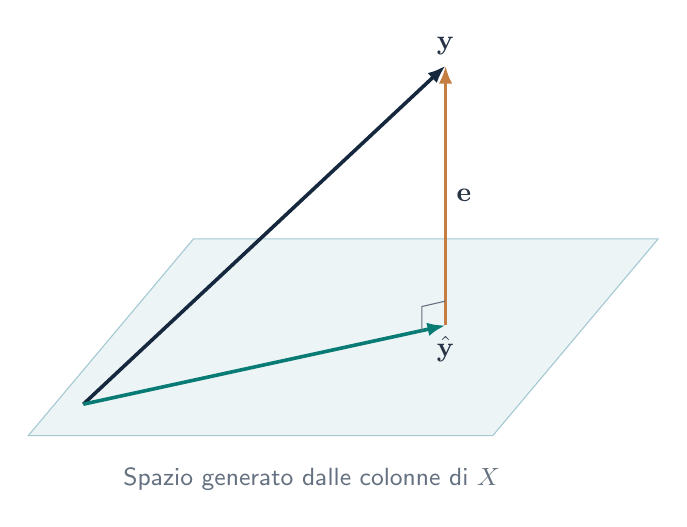
\begin{tikzpicture}[x=1cm,y=1cm]
\fill[GeoA!8](.8,.7)--(6.7,.7)--(8.8,3.2)--(2.9,3.2)--cycle;
\draw[GeoA!40](.8,.7)--(6.7,.7)--(8.8,3.2)--(2.9,3.2)--cycle;
\coordinate(o)at(1.5,1.1);\coordinate(yh)at(6.1,2.1);\coordinate(y)at(6.1,5.4);
\draw[pEdge,Navy,line width=1.3pt](o)--(y) node[above,pLabel]{$\mathbf y$};
\draw[pEdge,Classical,line width=1.3pt](o)--(yh) node[below,pLabel]{$\hat{\mathbf y}$};
\draw[pEdge,GeoB,line width=1.3pt](yh)--(y) node[midway,right,pLabel]{$\mathbf e$};
\draw[Muted](5.8,2.03)--(5.8,2.34)--(6.1,2.41);
\node[pNote] at(4.4,.15){Spazio generato dalle colonne di $X$};
\end{tikzpicture}

\end{minipage}%
\end{lrbox}
\typeout{FULLBOX:027:L:\the\ht\PilotLeftBox:\the\dp\PilotLeftBox}
\begin{lrbox}{\PilotRightBox}%
\begin{minipage}[t]{7.55cm}\raggedright\color{Ink}\fontsize{11.3}{14.8}\selectfont

\[X^\top(\mathbf y-X\hat{\boldsymbol\beta})=\mathbf0.\]
\PBody{Il residuo è ortogonale a ogni colonna del disegno. La previsione è il punto dello spazio del modello più vicino a $\mathbf y$.}
\[\hat{\boldsymbol\beta}=(X^\top X)^{-1}X^\top\mathbf y.\]
\PSmall{L’espressione con l’inversa richiede rango pieno. Il diagramma rappresenta uno spazio a $n$ dimensioni mediante uno schema tridimensionale.}

\end{minipage}%
\end{lrbox}
\typeout{FULLBOX:027:R:\the\ht\PilotRightBox:\the\dp\PilotRightBox}
\begin{tikzpicture}[remember picture,overlay]
\PilotChrome{I minimi quadrati sono una proiezione}{II · MODELLO LINEARE}{27}{L’ortogonalità dei residui esprime il criterio dei minimi quadrati in forma geometrica.}
\node[anchor=north west,inner sep=0] at([xshift=0.96cm,yshift=-2.13cm]current page.north west){\usebox{\PilotLeftBox}};
\node[anchor=north west,inner sep=0] at([xshift=11.52cm,yshift=-2.13cm]current page.north west){\usebox{\PilotRightBox}};
\end{tikzpicture}\end{frame}

\begin{frame}[plain]\hypertarget{slide28}{}
\bookmark[level=1,page=28]{La decomposizione QR esegue il calcolo}
\begin{lrbox}{\PilotLeftBox}%
\begin{minipage}[t]{10.05cm}\raggedright\color{Ink}\fontsize{11.3}{14.8}\selectfont

\[X=QR,\qquad Q^\top Q=I.\]
\[R\hat{\boldsymbol\beta}=Q^\top\mathbf y.\]
\begin{tikzpicture}[x=1cm,y=1cm]
\node[pFlow,text width=3.8cm] (a) at(2.3,2.8){Colonne di $X$\\predittori originali};
\node[pFlow,text width=3.8cm] (b) at(7.2,2.8){Colonne di $Q$\\base ortonormale};
\draw[pEdge](a)--(b);
\node[pNote,text width=8.5cm] at(4.8,.9){Un sistema triangolare in $R$ fornisce i coefficienti.};
\end{tikzpicture}

\end{minipage}%
\end{lrbox}
\typeout{FULLBOX:028:L:\the\ht\PilotLeftBox:\the\dp\PilotLeftBox}
\begin{lrbox}{\PilotRightBox}%
\begin{minipage}[t]{7.55cm}\raggedright\color{Ink}\fontsize{11.3}{14.8}\selectfont

\PCode{R · verificare stima e ortogonalità}{028_qr.R}
\PBody{La formula con l’inversa è utile per ragionare. Per il calcolo numerico \texttt{lm()} usa QR.}
\PInfo{Valori residui dell’ordine della precisione numerica sono compatibili con lo zero teorico. Il controllo usa tolleranze.}

\end{minipage}%
\end{lrbox}
\typeout{FULLBOX:028:R:\the\ht\PilotRightBox:\the\dp\PilotRightBox}
\begin{tikzpicture}[remember picture,overlay]
\PilotChrome{La decomposizione QR esegue il calcolo}{II · MODELLO LINEARE}{28}{Le formule spiegano il problema. Gli algoritmi numerici lo risolvono in modo stabile.}
\node[anchor=north west,inner sep=0] at([xshift=0.96cm,yshift=-2.13cm]current page.north west){\usebox{\PilotLeftBox}};
\node[anchor=north west,inner sep=0] at([xshift=11.52cm,yshift=-2.13cm]current page.north west){\usebox{\PilotRightBox}};
\end{tikzpicture}\end{frame}

\begin{frame}[plain]\hypertarget{slide29}{}
\bookmark[level=1,page=29]{Correlazione e pendenza sono collegate}
\begin{lrbox}{\PilotLeftBox}%
\begin{minipage}[t]{10.05cm}\raggedright\color{Ink}\fontsize{11.3}{14.8}\selectfont

\[\hat\beta_1=r\frac{s_y}{s_x}.\]
\begin{tikzpicture}[x=1cm,y=1cm]
\node[pFlow,text width=3.7cm] (a) at(2.3,3.3){$r$\\intensità e segno};
\node[pFlow,text width=3.7cm] (b) at(7.2,3.3){$s_y/s_x$\\rapporto delle scale};
\node[pLabel] (prodotto) at(4.8,1.2){Il prodotto restituisce la pendenza};
\draw[Classical,line width=.95pt](a.south)--(2.3,2.1)--(7.2,2.1)--(b.south);
\draw[pEdge](4.8,2.1)--(prodotto.north);
\end{tikzpicture}
\PInfo{L’identità $R^2=r^2$ riguarda la regressione semplice con intercetta. Nei modelli multipli non si trasferisce a una singola correlazione.}

\end{minipage}%
\end{lrbox}
\typeout{FULLBOX:029:L:\the\ht\PilotLeftBox:\the\dp\PilotLeftBox}
\begin{lrbox}{\PilotRightBox}%
\begin{minipage}[t]{7.55cm}\raggedright\color{Ink}\fontsize{11.3}{14.8}\selectfont

\PCode{R · controllare due identità}{029_identita.R}
\PBody{Se la dispersione della risposta raddoppia mentre $r$ resta uguale, la pendenza raddoppia a parità di $s_x$.}

\end{minipage}%
\end{lrbox}
\typeout{FULLBOX:029:R:\the\ht\PilotRightBox:\the\dp\PilotRightBox}
\begin{tikzpicture}[remember picture,overlay]
\PilotChrome{Correlazione e pendenza sono collegate}{II · MODELLO LINEARE}{29}{La pendenza conserva le scale delle variabili, mentre la correlazione le standardizza.}
\node[anchor=north west,inner sep=0] at([xshift=0.96cm,yshift=-2.13cm]current page.north west){\usebox{\PilotLeftBox}};
\node[anchor=north west,inner sep=0] at([xshift=11.52cm,yshift=-2.13cm]current page.north west){\usebox{\PilotRightBox}};
\end{tikzpicture}\end{frame}

\begin{frame}[plain]\hypertarget{slide30}{}
\bookmark[level=0,page=30]{Incertezza e previsione}
\bookmark[level=1,page=30]{La variabilità si scompone con l’intercetta}
\begin{lrbox}{\PilotLeftBox}%
\begin{minipage}[t]{10.05cm}\raggedright\color{Ink}\fontsize{11.3}{14.8}\selectfont

\[y_i-\bar y=(\hat y_i-\bar y)+e_i.\]
\[\underbrace{\sum_i(y_i-\bar y)^2}_{SST}
=\underbrace{\sum_i(\hat y_i-\bar y)^2}_{SSR}
+\underbrace{\sum_i e_i^2}_{SSE}.\]
\begin{tikzpicture}[x=1cm,y=1cm]
\fill[Classical!60](.5,1.5) rectangle(8.4,2.2);
\fill[GeoB!70](8.4,1.5) rectangle(9,2.2);
\node[pNote] at(4.3,1){variabilità della media stimata};
\node[pNote,text=GeoB,anchor=east] at(9,2.65){residua};
\end{tikzpicture}
\PSmall{La scomposizione usa l’ortogonalità dei residui. Vale per OLS con intercetta sugli stessi casi.}

\end{minipage}%
\end{lrbox}
\typeout{FULLBOX:030:L:\the\ht\PilotLeftBox:\the\dp\PilotLeftBox}
\begin{lrbox}{\PilotRightBox}%
\begin{minipage}[t]{7.55cm}\raggedright\color{Ink}\fontsize{11.3}{14.8}\selectfont

\PCode{R · verificare le somme dei quadrati}{030_scomposizione.R}
\PBody{Per i fossili, $SST=156{,}647$ e $SSE=10{,}646\ \mu\mathrm m^2$. Una retta riduce molto lo scarto rispetto alla sola media.}
\PInfo{Il confronto descrive l’adattamento sui dati usati per stimare il modello.}

\end{minipage}%
\end{lrbox}
\typeout{FULLBOX:030:R:\the\ht\PilotRightBox:\the\dp\PilotRightBox}
\begin{tikzpicture}[remember picture,overlay]
\PilotChrome{La variabilità si scompone con l’intercetta}{III · INCERTEZZA E PREVISIONE}{30}{La somma dei quadrati residua misura la parte rimasta attorno alla media stimata.}
\node[anchor=north west,inner sep=0] at([xshift=0.96cm,yshift=-2.13cm]current page.north west){\usebox{\PilotLeftBox}};
\node[anchor=north west,inner sep=0] at([xshift=11.52cm,yshift=-2.13cm]current page.north west){\usebox{\PilotRightBox}};
\end{tikzpicture}\end{frame}

\begin{frame}[plain]\hypertarget{slide31}{}
\bookmark[level=1,page=31]{R quadrato misura una riduzione relativa}
\begin{lrbox}{\PilotLeftBox}%
\begin{minipage}[t]{10.05cm}\raggedright\color{Ink}\fontsize{11.3}{14.8}\selectfont

\[R^2=1-\frac{SSE}{SST}=0{,}932.\]
\begin{tikzpicture}[x=1cm,y=1cm]
\draw[Rule,line width=12pt](.9,3.1)--(9,3.1);
\draw[Classical,line width=12pt](.9,3.1)--(8.449,3.1);
\node[pLabel] at(4.7,4.1){$93{,}2\%$ della somma dei quadrati};
\node[pNote] at(1,2.35){0};\node[pNote] at(9,2.35){1};
\node[pNote,text width=8.5cm] at(4.8,1){Confronto con la previsione costante $\bar y$};
\end{tikzpicture}

\end{minipage}%
\end{lrbox}
\typeout{FULLBOX:031:L:\the\ht\PilotLeftBox:\the\dp\PilotLeftBox}
\begin{lrbox}{\PilotRightBox}%
\begin{minipage}[t]{7.55cm}\raggedright\color{Ink}\fontsize{11.3}{14.8}\selectfont

\PBody{Nel campione, la retta riduce la somma dei quadrati del $93{,}2\%$ rispetto alla media.}
\PBody{Il valore non significa che il $93{,}2\%$ dei fossili abbia una previsione corretta. Per quantificare gli errori in micrometri serve una misura sulla scala della risposta.}
\PInfo{La relazione geometrica tra le variabili contribuisce al valore elevato di $R^2$.}

\end{minipage}%
\end{lrbox}
\typeout{FULLBOX:031:R:\the\ht\PilotRightBox:\the\dp\PilotRightBox}
\begin{tikzpicture}[remember picture,overlay]
\PilotChrome{R quadrato misura una riduzione relativa}{III · INCERTEZZA E PREVISIONE}{31}{R quadrato è una misura relativa di adattamento, riferita a una precisa risposta e a un preciso campione.}
\node[anchor=north west,inner sep=0] at([xshift=0.96cm,yshift=-2.13cm]current page.north west){\usebox{\PilotLeftBox}};
\node[anchor=north west,inner sep=0] at([xshift=11.52cm,yshift=-2.13cm]current page.north west){\usebox{\PilotRightBox}};
\end{tikzpicture}\end{frame}

\begin{frame}[plain]\hypertarget{slide32}{}
\bookmark[level=1,page=32]{Un R quadrato alto lascia aperte altre domande}
\begin{lrbox}{\PilotLeftBox}%
\begin{minipage}[t]{10.05cm}\raggedright\color{Ink}\fontsize{11.3}{14.8}\selectfont

\begin{tikzpicture}[x=1cm,y=1cm]
\node[pLabel,anchor=west] at(.7,4.8){Adattamento nel campione};
\draw[Classical,line width=4pt](.8,4.15)--(8.6,4.15);
\node[pLabel,anchor=west] at(.7,3.25){Forma corretta della relazione};
\node[pNote,anchor=west] at(.8,2.65){I residui possono mostrare una curvatura.};
\node[pLabel,anchor=west] at(.7,1.65){Previsione per nuovi casi};
\node[pNote,anchor=west] at(.8,1.05){Occorre osservare errori su dati esclusi dalla stima.};
\end{tikzpicture}

\end{minipage}%
\end{lrbox}
\typeout{FULLBOX:032:L:\the\ht\PilotLeftBox:\the\dp\PilotLeftBox}
\begin{lrbox}{\PilotRightBox}%
\begin{minipage}[t]{7.55cm}\raggedright\color{Ink}\fontsize{11.3}{14.8}\selectfont

\PBody{Aggiungendo termini a un modello OLS annidato, la somma dei quadrati nel training non aumenta. Il valore di $R^2$ può crescere anche con termini inutili.}
\PBody{Il confronto tra modelli deve quindi considerare diagnostica, complessità e prestazioni su nuovi casi.}
\PInfo{Per confrontare $R^2$ tra modelli, risposta e casi devono coincidere. Una trasformazione della risposta cambia il confronto.}

\end{minipage}%
\end{lrbox}
\typeout{FULLBOX:032:R:\the\ht\PilotRightBox:\the\dp\PilotRightBox}
\begin{tikzpicture}[remember picture,overlay]
\PilotChrome{Un R quadrato alto lascia aperte altre domande}{III · INCERTEZZA E PREVISIONE}{32}{La bontà dell’adattamento non basta per scegliere la complessità o sostenere una previsione.}
\node[anchor=north west,inner sep=0] at([xshift=0.96cm,yshift=-2.13cm]current page.north west){\usebox{\PilotLeftBox}};
\node[anchor=north west,inner sep=0] at([xshift=11.52cm,yshift=-2.13cm]current page.north west){\usebox{\PilotRightBox}};
\end{tikzpicture}\end{frame}

\begin{frame}[plain]\hypertarget{slide33}{}
\bookmark[level=1,page=33]{La dispersione residua conserva le unità}
\begin{lrbox}{\PilotLeftBox}%
\begin{minipage}[t]{10.05cm}\raggedright\color{Ink}\fontsize{11.3}{14.8}\selectfont

\[s^2=\frac{\sum_i e_i^2}{n-p},\qquad s=0{,}260\ \mu\mathrm m.\]
\begin{tikzpicture}[x=1cm,y=1cm]
\draw[pAxis](.6,2.6)--(9.2,2.6);
\draw[GeoA,line width=1.3pt,domain=.9:8.8,samples=65] plot(\x,{2.6+1.8*exp(-((\x-4.8)^2)/2)});
\draw[GeoB,line width=1.2pt](3.8,2.4)--(5.8,2.4);
\node[pNote] at(4.8,1.7){Scala degli scarti attorno alla media};
\node[pNote] at(4.8,4.9){Schema di errori a varianza costante};
\end{tikzpicture}

\end{minipage}%
\end{lrbox}
\typeout{FULLBOX:033:L:\the\ht\PilotLeftBox:\the\dp\PilotLeftBox}
\begin{lrbox}{\PilotRightBox}%
\begin{minipage}[t]{7.55cm}\raggedright\color{Ink}\fontsize{11.3}{14.8}\selectfont

\PCode{R · stimare la deviazione residua}{033_sigma.R}
\PBody{Si sottraggono i $p$ coefficienti stimati dai $n$ dati. Qui $n-p=158$. Sotto le ipotesi classiche, $s^2$ stima $\sigma^2$.}
\PInfo{$s$ e RMSE nel campione usano denominatori diversi. Entrambi sono espressi in micrometri, ma hanno ruoli differenti.}

\end{minipage}%
\end{lrbox}
\typeout{FULLBOX:033:R:\the\ht\PilotRightBox:\the\dp\PilotRightBox}
\begin{tikzpicture}[remember picture,overlay]
\PilotChrome{La dispersione residua conserva le unità}{III · INCERTEZZA E PREVISIONE}{33}{La deviazione residua misura una scala di variabilità condizionata, non l’errore della pendenza.}
\node[anchor=north west,inner sep=0] at([xshift=0.96cm,yshift=-2.13cm]current page.north west){\usebox{\PilotLeftBox}};
\node[anchor=north west,inner sep=0] at([xshift=11.52cm,yshift=-2.13cm]current page.north west){\usebox{\PilotRightBox}};
\end{tikzpicture}\end{frame}

\begin{frame}[plain]\hypertarget{slide34}{}
\bookmark[level=1,page=34]{La precisione della pendenza dipende dal disegno}
\begin{lrbox}{\PilotLeftBox}%
\begin{minipage}[t]{10.05cm}\raggedright\color{Ink}\fontsize{11.3}{14.8}\selectfont

\[\operatorname{SE}(\hat\beta_1)=\frac{s}{\sqrt{\sum_i(x_i-\bar x)^2}}.\]
\begin{tikzpicture}[x=1cm,y=1cm]
\draw[pAxis](.7,1.6)--(9,1.6);\draw[pAxis](.7,3.6)--(9,3.6);
\foreach \x in {3.6,3.85,4.1,4.35,4.6,4.85,5.1,5.35,5.6}{\fill[GeoB](\x,3.6) circle(2.8pt);}
\foreach \x in {1.1,2,2.9,3.8,4.7,5.6,6.5,7.4,8.3}{\fill[Classical](\x,1.6) circle(2.8pt);}
\node[pNote] at(4.8,4.3){predittore concentrato};
\node[pNote] at(4.8,.7){stesso numero di casi, campo più ampio};
\end{tikzpicture}

\end{minipage}%
\end{lrbox}
\typeout{FULLBOX:034:L:\the\ht\PilotLeftBox:\the\dp\PilotLeftBox}
\begin{lrbox}{\PilotRightBox}%
\begin{minipage}[t]{7.55cm}\raggedright\color{Ink}\fontsize{11.3}{14.8}\selectfont

\PBody{A parità di $s$, una maggiore dispersione di $X$ riduce l’errore standard della pendenza. Una maggiore variabilità residua lo aumenta.}
\PBody{Ampliare il campo di misura può migliorare la precisione, purché la forma del modello e la popolazione restino appropriate.}
\PInfo{La formula assume errori a varianza costante e non correlati. Con dipendenze spaziali o temporali occorre un modello della covarianza.}

\end{minipage}%
\end{lrbox}
\typeout{FULLBOX:034:R:\the\ht\PilotRightBox:\the\dp\PilotRightBox}
\begin{tikzpicture}[remember picture,overlay]
\PilotChrome{La precisione della pendenza dipende dal disegno}{III · INCERTEZZA E PREVISIONE}{34}{La precisione dipende sia dal numero di osservazioni sia da dove si trovano i predittori.}
\node[anchor=north west,inner sep=0] at([xshift=0.96cm,yshift=-2.13cm]current page.north west){\usebox{\PilotLeftBox}};
\node[anchor=north west,inner sep=0] at([xshift=11.52cm,yshift=-2.13cm]current page.north west){\usebox{\PilotRightBox}};
\end{tikzpicture}\end{frame}

\begin{frame}[plain]\hypertarget{slide35}{}
\bookmark[level=1,page=35]{Un intervallo accompagna la stima della pendenza}
\begin{lrbox}{\PilotLeftBox}%
\begin{minipage}[t]{10.05cm}\raggedright\color{Ink}\fontsize{11.3}{14.8}\selectfont

\[\hat\beta_1\pm t_{n-p,\,1-\alpha/2}\operatorname{SE}(\hat\beta_1).\]
\begin{tikzpicture}[x=1cm,y=1cm]
\draw[pAxis](.7,1.3)--(9.2,1.3);
\foreach \x/\lab in {1.2/{0,90},4.7/{0,95},8.2/{1,00}}{\node[pNote] at(\x,.8){$\lab$};}
\draw[Classical,line width=2pt](2.347,2.8)--(8.032,2.8);
\foreach \x in {2.347,8.032}{\draw[Classical](\x,2.55)--(\x,3.05);}
\fill[Classical](5.19,2.8) circle(3.3pt);
\node[pLabel] at(5.19,3.75){$0{,}957$};
\node[pNote] at(4.8,4.6){IC 95\%: $[0{,}916;\ 0{,}998]$};
\end{tikzpicture}
\PInfo{La copertura del 95\% riguarda la procedura in campioni ripetuti sotto le ipotesi, come discusso in Pelago.}

\end{minipage}%
\end{lrbox}
\typeout{FULLBOX:035:L:\the\ht\PilotLeftBox:\the\dp\PilotLeftBox}
\begin{lrbox}{\PilotRightBox}%
\begin{minipage}[t]{7.55cm}\raggedright\color{Ink}\fontsize{11.3}{14.8}\selectfont

\PCode{R · intervalli dei coefficienti}{035_ci_coef.R}
\PBody{L’intervallo descrive l’incertezza della pendenza nel modello dichiarato. Non incorpora automaticamente errori di misura, distorsioni del campionamento o una forma media sbagliata.}

\end{minipage}%
\end{lrbox}
\typeout{FULLBOX:035:R:\the\ht\PilotRightBox:\the\dp\PilotRightBox}
\begin{tikzpicture}[remember picture,overlay]
\PilotChrome{Un intervallo accompagna la stima della pendenza}{III · INCERTEZZA E PREVISIONE}{35}{Un intervallo richiede un parametro definito, una procedura e condizioni esplicite.}
\node[anchor=north west,inner sep=0] at([xshift=0.96cm,yshift=-2.13cm]current page.north west){\usebox{\PilotLeftBox}};
\node[anchor=north west,inner sep=0] at([xshift=11.52cm,yshift=-2.13cm]current page.north west){\usebox{\PilotRightBox}};
\end{tikzpicture}\end{frame}

\begin{frame}[plain]\hypertarget{slide36}{}
\bookmark[level=1,page=36]{L’intervallo per la risposta media}
\begin{lrbox}{\PilotLeftBox}%
\begin{minipage}[t]{10.05cm}\raggedright\color{Ink}\fontsize{11.3}{14.8}\selectfont

\PLabel{Media condizionata a un valore fissato}
\[\hat y_0=\hat\beta_0+\hat\beta_1x_0,\qquad
h_0=\frac1n+\frac{(x_0-\bar x)^2}{S_{xx}}.\]
\[\operatorname{SE}(\hat y_0)=s\sqrt{h_0}.\]
\[\boxed{\hat y_0\pm t_{n-p,\,1-\alpha/2}\,s\sqrt{h_0}}\]
\PBody{L’intervallo riguarda $E(Y\mid X=x_0)$. È più stretto vicino a $\bar x$, dove il disegno sostiene meglio la stima della media.}

\end{minipage}%
\end{lrbox}
\typeout{FULLBOX:036:L:\the\ht\PilotLeftBox:\the\dp\PilotLeftBox}
\begin{lrbox}{\PilotRightBox}%
\begin{minipage}[t]{7.55cm}\raggedright\color{Ink}\fontsize{11.3}{14.8}\selectfont

\begin{tikzpicture}[x=1cm,y=1cm]
\draw[pAxis](.6,.7)--(7,.7);\draw[pAxis](.6,.7)--(.6,5.3);
\draw[Classical,line width=1.2pt](1,1.4)--(6.6,4.3);
\foreach \x/\y/\s in {1.4/1.61/.55,3.8/2.85/.22,6.2/4.09/.55}{\draw[GeoB,line width=2pt](\x,\y-\s)--(\x,\y+\s);\fill[Classical](\x,\y) circle(2pt);}
\node[pNote] at(3.8,.25){$\bar x$};
\node[pNote,text width=6.2cm] at(3.8,5.65){Schema di intervalli della media};
\end{tikzpicture}
\PSmall{Per un modello multiplo, $h_0=\mathbf x_0^\top(X^\top X)^{-1}\mathbf x_0$, con intercetta inclusa in $\mathbf x_0$.}

\end{minipage}%
\end{lrbox}
\typeout{FULLBOX:036:R:\the\ht\PilotRightBox:\the\dp\PilotRightBox}
\begin{tikzpicture}[remember picture,overlay]
\PilotChrome{L’intervallo per la risposta media}{III · INCERTEZZA E PREVISIONE}{36}{L’intervallo della media quantifica l’incertezza sulla posizione della funzione media.}
\node[anchor=north west,inner sep=0] at([xshift=0.96cm,yshift=-2.13cm]current page.north west){\usebox{\PilotLeftBox}};
\node[anchor=north west,inner sep=0] at([xshift=11.52cm,yshift=-2.13cm]current page.north west){\usebox{\PilotRightBox}};
\end{tikzpicture}\end{frame}

\begin{frame}[plain]\hypertarget{slide37}{}
\bookmark[level=1,page=37]{Un nuovo individuo aggiunge la propria variabilità}
\begin{lrbox}{\PilotLeftBox}%
\begin{minipage}[t]{10.05cm}\raggedright\color{Ink}\fontsize{11.3}{14.8}\selectfont

\[Y_{\rm nuovo}-\hat y_0=\varepsilon_{\rm nuovo}+
\{E(Y\mid x_0)-\hat y_0\}.\]
\[\operatorname{SE}_{\rm pred}=s\sqrt{1+h_0}.\]
\[\boxed{\hat y_0\pm t_{n-p,\,1-\alpha/2}\,s\sqrt{1+h_0}}\]
\PBody{Il termine $1$ corrisponde alla variabilità del nuovo individuo. L’altro termine riguarda la stima della media.}

\end{minipage}%
\end{lrbox}
\typeout{FULLBOX:037:L:\the\ht\PilotLeftBox:\the\dp\PilotLeftBox}
\begin{lrbox}{\PilotRightBox}%
\begin{minipage}[t]{7.55cm}\raggedright\color{Ink}\fontsize{11.3}{14.8}\selectfont

\begin{tikzpicture}[x=1cm,y=1cm]
\draw[pAxis](.7,2.5)--(7,2.5);
\draw[GeoA!50,line width=7pt](1.1,3.8)--(6.6,3.8);
\draw[Classical,line width=7pt](3.2,1.3)--(4.5,1.3);
\fill[Navy](3.85,3.8) circle(3pt);\fill[Navy](3.85,1.3) circle(3pt);
\node[pNote] at(3.85,4.5){nuovo individuo};
\node[pNote] at(3.85,.55){risposta media};
\end{tikzpicture}
\PInfo{La previsione classica assume un nuovo errore indipendente, con la stessa varianza. La normalità rende esatta la copertura t a campione finito.}

\end{minipage}%
\end{lrbox}
\typeout{FULLBOX:037:R:\the\ht\PilotRightBox:\the\dp\PilotRightBox}
\begin{tikzpicture}[remember picture,overlay]
\PilotChrome{Un nuovo individuo aggiunge la propria variabilità}{III · INCERTEZZA E PREVISIONE}{37}{Una media stimata con precisione può convivere con una forte variabilità individuale.}
\node[anchor=north west,inner sep=0] at([xshift=0.96cm,yshift=-2.13cm]current page.north west){\usebox{\PilotLeftBox}};
\node[anchor=north west,inner sep=0] at([xshift=11.52cm,yshift=-2.13cm]current page.north west){\usebox{\PilotRightBox}};
\end{tikzpicture}\end{frame}

\begin{frame}[plain]\hypertarget{slide38}{}
\bookmark[level=1,page=38]{Le due bande rispondono a domande differenti}
\begin{lrbox}{\PilotLeftBox}%
\begin{minipage}[t]{10.05cm}\raggedright\color{Ink}\fontsize{11.3}{14.8}\selectfont
\begin{tikzpicture}[x=1cm,y=1cm]
\path[use as bounding box](-.25,-.4) rectangle(9.15,4.7);
\draw[pAxis](.65,.65)--(9,.65);
\draw[pAxis](.65,.65)--(.65,4.5);
\draw[Muted](0.6500,.59)--(0.6500,.71);\node[pNote] at(0.6500,.31){$ 3 $};
\draw[Muted](1.9583,.59)--(1.9583,.71);\node[pNote] at(1.9583,.31){$ 4 $};
\draw[Muted](3.2667,.59)--(3.2667,.71);\node[pNote] at(3.2667,.31){$ 5 $};
\draw[Muted](4.5750,.59)--(4.5750,.71);\node[pNote] at(4.5750,.31){$ 6 $};
\draw[Muted](5.8833,.59)--(5.8833,.71);\node[pNote] at(5.8833,.31){$ 7 $};
\draw[Muted](7.1917,.59)--(7.1917,.71);\node[pNote] at(7.1917,.31){$ 8 $};
\draw[Muted](8.5000,.59)--(8.5000,.71);\node[pNote] at(8.5000,.31){$ 9 $};
\draw[Muted](.59,0.6500)--(.71,0.6500);\node[pNote,anchor=east] at(.5,0.6500){$ 2 $};
\draw[Muted](.59,1.8500)--(.71,1.8500);\node[pNote,anchor=east] at(.5,1.8500){$ 4 $};
\draw[Muted](.59,3.0500)--(.71,3.0500);\node[pNote,anchor=east] at(.5,3.0500){$ 6 $};
\draw[Muted](.59,4.2500)--(.71,4.2500);\node[pNote,anchor=east] at(.5,4.2500){$ 8 $};
\node[pNote] at(4.9,-.15){Diametro totale ($\mu$m)};
\node[pNote,rotate=90] at(-.14,2.55){Diametro interno ($\mu$m)};
\fill[GeoA!13] (1.5369,0.8263)--(1.5908,0.8501)--(1.6447,0.8740)--(1.6986,0.8978)--(1.7525,0.9217)--(1.8064,0.9455)--(1.8603,0.9694)--(1.9142,0.9932)--(1.9681,1.0171)--(2.0219,1.0409)--(2.0758,1.0647)--(2.1297,1.0886)--(2.1836,1.1124)--(2.2375,1.1362)--(2.2914,1.1600)--(2.3453,1.1838)--(2.3992,1.2076)--(2.4531,1.2315)--(2.5070,1.2553)--(2.5609,1.2791)--(2.6148,1.3029)--(2.6687,1.3267)--(2.7226,1.3505)--(2.7765,1.3742)--(2.8304,1.3980)--(2.8842,1.4218)--(2.9381,1.4456)--(2.9920,1.4694)--(3.0459,1.4931)--(3.0998,1.5169)--(3.1537,1.5407)--(3.2076,1.5644)--(3.2615,1.5882)--(3.3154,1.6120)--(3.3693,1.6357)--(3.4232,1.6595)--(3.4771,1.6832)--(3.5310,1.7070)--(3.5849,1.7307)--(3.6388,1.7544)--(3.6926,1.7782)--(3.7465,1.8019)--(3.8004,1.8256)--(3.8543,1.8494)--(3.9082,1.8731)--(3.9621,1.8968)--(4.0160,1.9205)--(4.0699,1.9442)--(4.1238,1.9680)--(4.1777,1.9917)--(4.2316,2.0154)--(4.2855,2.0391)--(4.3394,2.0628)--(4.3933,2.0865)--(4.4472,2.1101)--(4.5010,2.1338)--(4.5549,2.1575)--(4.6088,2.1812)--(4.6627,2.2049)--(4.7166,2.2285)--(4.7705,2.2522)--(4.8244,2.2759)--(4.8783,2.2995)--(4.9322,2.3232)--(4.9861,2.3469)--(5.0400,2.3705)--(5.0939,2.3942)--(5.1478,2.4178)--(5.2017,2.4415)--(5.2556,2.4651)--(5.3094,2.4887)--(5.3633,2.5124)--(5.4172,2.5360)--(5.4711,2.5596)--(5.5250,2.5833)--(5.5789,2.6069)--(5.6328,2.6305)--(5.6867,2.6541)--(5.7406,2.6777)--(5.7945,2.7013)--(5.8484,2.7249)--(5.9023,2.7485)--(5.9562,2.7721)--(6.0101,2.7957)--(6.0640,2.8193)--(6.1178,2.8429)--(6.1717,2.8665)--(6.2256,2.8901)--(6.2795,2.9137)--(6.3334,2.9372)--(6.3873,2.9608)--(6.4412,2.9844)--(6.4951,3.0079)--(6.5490,3.0315)--(6.6029,3.0551)--(6.6568,3.0786)--(6.7107,3.1022)--(6.7646,3.1257)--(6.8185,3.1493)--(6.8724,3.1728)--(6.9262,3.1964)--(6.9801,3.2199)--(7.0340,3.2434)--(7.0879,3.2670)--(7.1418,3.2905)--(7.1957,3.3140)--(7.2496,3.3375)--(7.3035,3.3611)--(7.3574,3.3846)--(7.4113,3.4081)--(7.4652,3.4316)--(7.5191,3.4551)--(7.5730,3.4786)--(7.6269,3.5021)--(7.6808,3.5256)--(7.7346,3.5491)--(7.7885,3.5726)--(7.8424,3.5961)--(7.8963,3.6195)--(7.9502,3.6430)--(8.0041,3.6665)--(8.0041,4.2935)--(7.9502,4.2696)--(7.8963,4.2458)--(7.8424,4.2220)--(7.7885,4.1982)--(7.7346,4.1743)--(7.6808,4.1505)--(7.6269,4.1267)--(7.5730,4.1029)--(7.5191,4.0791)--(7.4652,4.0553)--(7.4113,4.0315)--(7.3574,4.0077)--(7.3035,3.9839)--(7.2496,3.9602)--(7.1957,3.9364)--(7.1418,3.9126)--(7.0879,3.8888)--(7.0340,3.8650)--(6.9801,3.8413)--(6.9262,3.8175)--(6.8724,3.7937)--(6.8185,3.7700)--(6.7646,3.7462)--(6.7107,3.7225)--(6.6568,3.6987)--(6.6029,3.6750)--(6.5490,3.6512)--(6.4951,3.6275)--(6.4412,3.6037)--(6.3873,3.5800)--(6.3334,3.5563)--(6.2795,3.5325)--(6.2256,3.5088)--(6.1717,3.4851)--(6.1178,3.4614)--(6.0640,3.4377)--(6.0101,3.4139)--(5.9562,3.3902)--(5.9023,3.3665)--(5.8484,3.3428)--(5.7945,3.3191)--(5.7406,3.2954)--(5.6867,3.2717)--(5.6328,3.2480)--(5.5789,3.2244)--(5.5250,3.2007)--(5.4711,3.1770)--(5.4172,3.1533)--(5.3633,3.1296)--(5.3094,3.1060)--(5.2556,3.0823)--(5.2017,3.0586)--(5.1478,3.0350)--(5.0939,3.0113)--(5.0400,2.9877)--(4.9861,2.9640)--(4.9322,2.9404)--(4.8783,2.9167)--(4.8244,2.8931)--(4.7705,2.8694)--(4.7166,2.8458)--(4.6627,2.8222)--(4.6088,2.7985)--(4.5549,2.7749)--(4.5010,2.7513)--(4.4472,2.7277)--(4.3933,2.7041)--(4.3394,2.6805)--(4.2855,2.6568)--(4.2316,2.6332)--(4.1777,2.6096)--(4.1238,2.5860)--(4.0699,2.5624)--(4.0160,2.5389)--(3.9621,2.5153)--(3.9082,2.4917)--(3.8543,2.4681)--(3.8004,2.4445)--(3.7465,2.4209)--(3.6926,2.3974)--(3.6388,2.3738)--(3.5849,2.3502)--(3.5310,2.3267)--(3.4771,2.3031)--(3.4232,2.2795)--(3.3693,2.2560)--(3.3154,2.2324)--(3.2615,2.2089)--(3.2076,2.1854)--(3.1537,2.1618)--(3.0998,2.1383)--(3.0459,2.1147)--(2.9920,2.0912)--(2.9381,2.0677)--(2.8842,2.0442)--(2.8304,2.0206)--(2.7765,1.9971)--(2.7226,1.9736)--(2.6687,1.9501)--(2.6148,1.9266)--(2.5609,1.9031)--(2.5070,1.8796)--(2.4531,1.8561)--(2.3992,1.8326)--(2.3453,1.8091)--(2.2914,1.7856)--(2.2375,1.7621)--(2.1836,1.7386)--(2.1297,1.7151)--(2.0758,1.6917)--(2.0219,1.6682)--(1.9681,1.6447)--(1.9142,1.6213)--(1.8603,1.5978)--(1.8064,1.5743)--(1.7525,1.5509)--(1.6986,1.5274)--(1.6447,1.5040)--(1.5908,1.4805)--(1.5369,1.4571)--cycle;
\fill[Classical!35] (1.5369,1.0721)--(1.5908,1.0967)--(1.6447,1.1213)--(1.6986,1.1458)--(1.7525,1.1704)--(1.8064,1.1950)--(1.8603,1.2196)--(1.9142,1.2442)--(1.9681,1.2687)--(2.0219,1.2933)--(2.0758,1.3179)--(2.1297,1.3425)--(2.1836,1.3670)--(2.2375,1.3916)--(2.2914,1.4162)--(2.3453,1.4407)--(2.3992,1.4653)--(2.4531,1.4898)--(2.5070,1.5144)--(2.5609,1.5389)--(2.6148,1.5634)--(2.6687,1.5880)--(2.7226,1.6125)--(2.7765,1.6370)--(2.8304,1.6616)--(2.8842,1.6861)--(2.9381,1.7106)--(2.9920,1.7351)--(3.0459,1.7596)--(3.0998,1.7841)--(3.1537,1.8085)--(3.2076,1.8330)--(3.2615,1.8575)--(3.3154,1.8819)--(3.3693,1.9064)--(3.4232,1.9308)--(3.4771,1.9553)--(3.5310,1.9797)--(3.5849,2.0041)--(3.6388,2.0285)--(3.6926,2.0528)--(3.7465,2.0772)--(3.8004,2.1016)--(3.8543,2.1259)--(3.9082,2.1502)--(3.9621,2.1745)--(4.0160,2.1988)--(4.0699,2.2231)--(4.1238,2.2473)--(4.1777,2.2715)--(4.2316,2.2957)--(4.2855,2.3199)--(4.3394,2.3440)--(4.3933,2.3681)--(4.4472,2.3922)--(4.5010,2.4163)--(4.5549,2.4403)--(4.6088,2.4643)--(4.6627,2.4882)--(4.7166,2.5121)--(4.7705,2.5360)--(4.8244,2.5598)--(4.8783,2.5836)--(4.9322,2.6074)--(4.9861,2.6311)--(5.0400,2.6548)--(5.0939,2.6784)--(5.1478,2.7020)--(5.2017,2.7255)--(5.2556,2.7490)--(5.3094,2.7725)--(5.3633,2.7959)--(5.4172,2.8193)--(5.4711,2.8427)--(5.5250,2.8660)--(5.5789,2.8893)--(5.6328,2.9126)--(5.6867,2.9358)--(5.7406,2.9590)--(5.7945,2.9821)--(5.8484,3.0053)--(5.9023,3.0284)--(5.9562,3.0515)--(6.0101,3.0745)--(6.0640,3.0976)--(6.1178,3.1206)--(6.1717,3.1436)--(6.2256,3.1666)--(6.2795,3.1896)--(6.3334,3.2125)--(6.3873,3.2354)--(6.4412,3.2584)--(6.4951,3.2813)--(6.5490,3.3042)--(6.6029,3.3271)--(6.6568,3.3500)--(6.7107,3.3728)--(6.7646,3.3957)--(6.8185,3.4185)--(6.8724,3.4414)--(6.9262,3.4642)--(6.9801,3.4870)--(7.0340,3.5098)--(7.0879,3.5326)--(7.1418,3.5554)--(7.1957,3.5782)--(7.2496,3.6010)--(7.3035,3.6238)--(7.3574,3.6466)--(7.4113,3.6694)--(7.4652,3.6921)--(7.5191,3.7149)--(7.5730,3.7377)--(7.6269,3.7604)--(7.6808,3.7832)--(7.7346,3.8059)--(7.7885,3.8287)--(7.8424,3.8514)--(7.8963,3.8742)--(7.9502,3.8969)--(8.0041,3.9196)--(8.0041,4.0403)--(7.9502,4.0157)--(7.8963,3.9912)--(7.8424,3.9666)--(7.7885,3.9421)--(7.7346,3.9175)--(7.6808,3.8929)--(7.6269,3.8684)--(7.5730,3.8438)--(7.5191,3.8193)--(7.4652,3.7948)--(7.4113,3.7702)--(7.3574,3.7457)--(7.3035,3.7212)--(7.2496,3.6967)--(7.1957,3.6721)--(7.1418,3.6476)--(7.0879,3.6231)--(7.0340,3.5986)--(6.9801,3.5741)--(6.9262,3.5497)--(6.8724,3.5252)--(6.8185,3.5007)--(6.7646,3.4763)--(6.7107,3.4518)--(6.6568,3.4274)--(6.6029,3.4030)--(6.5490,3.3785)--(6.4951,3.3541)--(6.4412,3.3297)--(6.3873,3.3054)--(6.3334,3.2810)--(6.2795,3.2566)--(6.2256,3.2323)--(6.1717,3.2080)--(6.1178,3.1837)--(6.0640,3.1594)--(6.0101,3.1351)--(5.9562,3.1109)--(5.9023,3.0867)--(5.8484,3.0625)--(5.7945,3.0383)--(5.7406,3.0142)--(5.6867,2.9901)--(5.6328,2.9660)--(5.5789,2.9419)--(5.5250,2.9179)--(5.4711,2.8939)--(5.4172,2.8700)--(5.3633,2.8461)--(5.3094,2.8222)--(5.2556,2.7984)--(5.2017,2.7746)--(5.1478,2.7508)--(5.0939,2.7271)--(5.0400,2.7034)--(4.9861,2.6798)--(4.9322,2.6562)--(4.8783,2.6326)--(4.8244,2.6091)--(4.7705,2.5857)--(4.7166,2.5622)--(4.6627,2.5388)--(4.6088,2.5155)--(4.5549,2.4922)--(4.5010,2.4689)--(4.4472,2.4456)--(4.3933,2.4224)--(4.3394,2.3992)--(4.2855,2.3760)--(4.2316,2.3529)--(4.1777,2.3298)--(4.1238,2.3067)--(4.0699,2.2836)--(4.0160,2.2606)--(3.9621,2.2376)--(3.9082,2.2146)--(3.8543,2.1916)--(3.8004,2.1686)--(3.7465,2.1456)--(3.6926,2.1227)--(3.6388,2.0998)--(3.5849,2.0769)--(3.5310,2.0540)--(3.4771,2.0311)--(3.4232,2.0082)--(3.3693,1.9853)--(3.3154,1.9625)--(3.2615,1.9396)--(3.2076,1.9168)--(3.1537,1.8940)--(3.0998,1.8711)--(3.0459,1.8483)--(2.9920,1.8255)--(2.9381,1.8027)--(2.8842,1.7799)--(2.8304,1.7571)--(2.7765,1.7343)--(2.7226,1.7115)--(2.6687,1.6888)--(2.6148,1.6660)--(2.5609,1.6432)--(2.5070,1.6205)--(2.4531,1.5977)--(2.3992,1.5750)--(2.3453,1.5522)--(2.2914,1.5295)--(2.2375,1.5067)--(2.1836,1.4840)--(2.1297,1.4612)--(2.0758,1.4385)--(2.0219,1.4158)--(1.9681,1.3930)--(1.9142,1.3703)--(1.8603,1.3476)--(1.8064,1.3249)--(1.7525,1.3021)--(1.6986,1.2794)--(1.6447,1.2567)--(1.5908,1.2340)--(1.5369,1.2113)--cycle;
\fill[GeoA,opacity=.68](6.1897,3.2611) circle(1.25pt);
\fill[GeoA,opacity=.68](4.3267,2.4540) circle(1.25pt);
\fill[GeoA,opacity=.68](5.4096,2.8289) circle(1.25pt);
\fill[GeoA,opacity=.68](2.3576,1.5515) circle(1.25pt);
\fill[GeoA,opacity=.68](5.0513,2.8602) circle(1.25pt);
\fill[GeoA,opacity=.68](5.8011,3.1340) circle(1.25pt);
\fill[GeoA,opacity=.68](4.9498,2.4739) circle(1.25pt);
\fill[GeoA,opacity=.68](5.5533,2.7720) circle(1.25pt);
\fill[GeoA,opacity=.68](3.1051,1.8535) circle(1.25pt);
\fill[GeoA,opacity=.68](4.9363,2.5274) circle(1.25pt);
\fill[GeoA,opacity=.68](4.4363,2.1680) circle(1.25pt);
\fill[GeoA,opacity=.68](4.5694,2.6032) circle(1.25pt);
\fill[GeoA,opacity=.68](2.9003,1.7582) circle(1.25pt);
\fill[GeoA,opacity=.68](1.8549,1.1055) circle(1.25pt);
\fill[GeoA,opacity=.68](5.7031,2.9335) circle(1.25pt);
\fill[GeoA,opacity=.68](6.4093,3.4399) circle(1.25pt);
\fill[GeoA,opacity=.68](2.7501,1.9638) circle(1.25pt);
\fill[GeoA,opacity=.68](5.0777,2.7140) circle(1.25pt);
\fill[GeoA,opacity=.68](6.4083,3.3364) circle(1.25pt);
\fill[GeoA,opacity=.68](4.6548,2.7043) circle(1.25pt);
\fill[GeoA,opacity=.68](5.1658,2.7778) circle(1.25pt);
\fill[GeoA,opacity=.68](4.9778,2.7777) circle(1.25pt);
\fill[GeoA,opacity=.68](3.0769,1.9963) circle(1.25pt);
\fill[GeoA,opacity=.68](3.4405,2.1627) circle(1.25pt);
\fill[GeoA,opacity=.68](5.3290,3.0129) circle(1.25pt);
\fill[GeoA,opacity=.68](6.4214,3.5817) circle(1.25pt);
\fill[GeoA,opacity=.68](2.7120,1.7399) circle(1.25pt);
\fill[GeoA,opacity=.68](4.4141,2.6920) circle(1.25pt);
\fill[GeoA,opacity=.68](6.6143,3.4658) circle(1.25pt);
\fill[GeoA,opacity=.68](3.2947,1.8672) circle(1.25pt);
\fill[GeoA,opacity=.68](4.5810,2.4570) circle(1.25pt);
\fill[GeoA,opacity=.68](2.9884,1.8006) circle(1.25pt);
\fill[GeoA,opacity=.68](5.3587,3.0130) circle(1.25pt);
\fill[GeoA,opacity=.68](6.9579,3.7831) circle(1.25pt);
\fill[GeoA,opacity=.68](3.6469,2.1159) circle(1.25pt);
\fill[GeoA,opacity=.68](3.2736,1.9108) circle(1.25pt);
\fill[GeoA,opacity=.68](2.7672,1.7359) circle(1.25pt);
\fill[GeoA,opacity=.68](4.8663,2.5441) circle(1.25pt);
\fill[GeoA,opacity=.68](4.4756,2.7386) circle(1.25pt);
\fill[GeoA,opacity=.68](1.7650,1.4292) circle(1.25pt);
\fill[GeoA,opacity=.68](5.4928,3.0116) circle(1.25pt);
\fill[GeoA,opacity=.68](3.8415,2.4811) circle(1.25pt);
\fill[GeoA,opacity=.68](5.4655,2.9759) circle(1.25pt);
\fill[GeoA,opacity=.68](5.6580,3.1958) circle(1.25pt);
\fill[GeoA,opacity=.68](3.1668,1.8214) circle(1.25pt);
\fill[GeoA,opacity=.68](6.5804,3.2407) circle(1.25pt);
\fill[GeoA,opacity=.68](5.5215,3.1531) circle(1.25pt);
\fill[GeoA,opacity=.68](4.2664,2.3435) circle(1.25pt);
\fill[GeoA,opacity=.68](3.4480,2.0425) circle(1.25pt);
\fill[GeoA,opacity=.68](4.7386,2.7491) circle(1.25pt);
\fill[GeoA,opacity=.68](2.7137,1.6439) circle(1.25pt);
\fill[GeoA,opacity=.68](5.1706,2.8687) circle(1.25pt);
\fill[GeoA,opacity=.68](2.5419,1.3358) circle(1.25pt);
\fill[GeoA,opacity=.68](2.9290,1.5615) circle(1.25pt);
\fill[GeoA,opacity=.68](5.2026,2.9308) circle(1.25pt);
\fill[GeoA,opacity=.68](6.6109,3.2625) circle(1.25pt);
\fill[GeoA,opacity=.68](5.3589,2.8067) circle(1.25pt);
\fill[GeoA,opacity=.68](6.0434,3.2227) circle(1.25pt);
\fill[GeoA,opacity=.68](4.9067,2.2528) circle(1.25pt);
\fill[GeoA,opacity=.68](5.4016,2.7996) circle(1.25pt);
\fill[GeoA,opacity=.68](5.9133,3.1398) circle(1.25pt);
\fill[GeoA,opacity=.68](5.8798,2.9729) circle(1.25pt);
\fill[GeoA,opacity=.68](5.2871,2.9693) circle(1.25pt);
\fill[GeoA,opacity=.68](4.3058,2.3370) circle(1.25pt);
\fill[GeoA,opacity=.68](3.7786,1.9608) circle(1.25pt);
\fill[GeoA,opacity=.68](4.9535,2.7637) circle(1.25pt);
\fill[GeoA,opacity=.68](6.1374,3.3113) circle(1.25pt);
\fill[GeoA,opacity=.68](5.2695,2.7792) circle(1.25pt);
\fill[GeoA,opacity=.68](7.5178,3.6952) circle(1.25pt);
\fill[GeoA,opacity=.68](3.8817,2.4202) circle(1.25pt);
\fill[GeoA,opacity=.68](4.9197,2.9737) circle(1.25pt);
\fill[GeoA,opacity=.68](4.9469,2.6185) circle(1.25pt);
\fill[GeoA,opacity=.68](6.5873,3.4427) circle(1.25pt);
\fill[GeoA,opacity=.68](5.1065,2.7262) circle(1.25pt);
\fill[GeoA,opacity=.68](1.9571,1.1992) circle(1.25pt);
\fill[GeoA,opacity=.68](4.5615,2.5558) circle(1.25pt);
\fill[GeoA,opacity=.68](3.4190,1.8898) circle(1.25pt);
\fill[GeoA,opacity=.68](5.3289,3.1911) circle(1.25pt);
\fill[GeoA,opacity=.68](4.4386,2.4850) circle(1.25pt);
\fill[GeoA,opacity=.68](4.8386,2.7592) circle(1.25pt);
\fill[GeoB,opacity=.68](6.5006,3.3581) circle(1.25pt);
\fill[GeoB,opacity=.68](5.9671,2.8508) circle(1.25pt);
\fill[GeoB,opacity=.68](3.9187,2.0952) circle(1.25pt);
\fill[GeoB,opacity=.68](5.4185,3.0106) circle(1.25pt);
\fill[GeoB,opacity=.68](4.7241,2.5008) circle(1.25pt);
\fill[GeoB,opacity=.68](4.5318,2.5036) circle(1.25pt);
\fill[GeoB,opacity=.68](5.7043,2.8167) circle(1.25pt);
\fill[GeoB,opacity=.68](3.9125,2.1987) circle(1.25pt);
\fill[GeoB,opacity=.68](7.5265,3.6140) circle(1.25pt);
\fill[GeoB,opacity=.68](3.3767,1.7489) circle(1.25pt);
\fill[GeoB,opacity=.68](1.5369,0.9396) circle(1.25pt);
\fill[GeoB,opacity=.68](6.0301,2.9892) circle(1.25pt);
\fill[GeoB,opacity=.68](4.5873,2.3466) circle(1.25pt);
\fill[GeoB,opacity=.68](4.0787,2.2087) circle(1.25pt);
\fill[GeoB,opacity=.68](7.1656,3.6762) circle(1.25pt);
\fill[GeoB,opacity=.68](4.7584,2.7077) circle(1.25pt);
\fill[GeoB,opacity=.68](6.9273,3.5279) circle(1.25pt);
\fill[GeoB,opacity=.68](6.4365,3.5426) circle(1.25pt);
\fill[GeoB,opacity=.68](5.1891,2.4904) circle(1.25pt);
\fill[GeoB,opacity=.68](4.4335,2.3018) circle(1.25pt);
\fill[GeoB,opacity=.68](4.2498,2.2202) circle(1.25pt);
\fill[GeoB,opacity=.68](6.7371,3.1209) circle(1.25pt);
\fill[GeoB,opacity=.68](4.2805,2.2188) circle(1.25pt);
\fill[GeoB,opacity=.68](6.6270,3.2770) circle(1.25pt);
\fill[GeoB,opacity=.68](5.0825,2.6623) circle(1.25pt);
\fill[GeoB,opacity=.68](3.4635,1.9370) circle(1.25pt);
\fill[GeoB,opacity=.68](5.5779,2.7133) circle(1.25pt);
\fill[GeoB,opacity=.68](3.9263,2.0835) circle(1.25pt);
\fill[GeoB,opacity=.68](4.0271,1.9865) circle(1.25pt);
\fill[GeoB,opacity=.68](5.9945,3.1245) circle(1.25pt);
\fill[GeoB,opacity=.68](5.1824,2.9133) circle(1.25pt);
\fill[GeoB,opacity=.68](3.5151,1.9164) circle(1.25pt);
\fill[GeoB,opacity=.68](5.9418,2.6273) circle(1.25pt);
\fill[GeoB,opacity=.68](4.7301,2.6119) circle(1.25pt);
\fill[GeoB,opacity=.68](4.5091,2.4191) circle(1.25pt);
\fill[GeoB,opacity=.68](5.2670,3.0811) circle(1.25pt);
\fill[GeoB,opacity=.68](7.0385,3.5655) circle(1.25pt);
\fill[GeoB,opacity=.68](6.3949,3.4414) circle(1.25pt);
\fill[GeoB,opacity=.68](6.5240,3.2203) circle(1.25pt);
\fill[GeoB,opacity=.68](8.0041,3.9996) circle(1.25pt);
\fill[GeoB,opacity=.68](3.6224,1.9612) circle(1.25pt);
\fill[GeoB,opacity=.68](5.0465,2.8610) circle(1.25pt);
\fill[GeoB,opacity=.68](6.3766,3.2450) circle(1.25pt);
\fill[GeoB,opacity=.68](7.0138,3.3370) circle(1.25pt);
\fill[GeoB,opacity=.68](5.3403,2.6413) circle(1.25pt);
\fill[GeoB,opacity=.68](5.2813,2.5876) circle(1.25pt);
\fill[GeoB,opacity=.68](5.0621,2.4857) circle(1.25pt);
\fill[GeoB,opacity=.68](5.7532,2.8526) circle(1.25pt);
\fill[GeoB,opacity=.68](4.8650,2.5564) circle(1.25pt);
\fill[GeoB,opacity=.68](4.5255,2.6209) circle(1.25pt);
\fill[GeoB,opacity=.68](4.7418,2.2794) circle(1.25pt);
\fill[GeoB,opacity=.68](5.4990,2.7924) circle(1.25pt);
\fill[GeoB,opacity=.68](7.1289,3.8002) circle(1.25pt);
\fill[GeoB,opacity=.68](5.3809,2.8132) circle(1.25pt);
\fill[GeoB,opacity=.68](5.8926,3.0732) circle(1.25pt);
\fill[GeoB,opacity=.68](5.5543,2.7911) circle(1.25pt);
\fill[GeoB,opacity=.68](7.3231,3.6000) circle(1.25pt);
\fill[GeoB,opacity=.68](2.7132,1.5682) circle(1.25pt);
\fill[GeoB,opacity=.68](5.2061,2.5533) circle(1.25pt);
\fill[GeoB,opacity=.68](6.6354,3.2852) circle(1.25pt);
\fill[GeoB,opacity=.68](7.3104,3.6713) circle(1.25pt);
\fill[GeoB,opacity=.68](6.2228,2.9929) circle(1.25pt);
\fill[GeoB,opacity=.68](4.9225,2.5265) circle(1.25pt);
\fill[GeoB,opacity=.68](7.2759,3.6028) circle(1.25pt);
\fill[GeoB,opacity=.68](3.9329,2.1139) circle(1.25pt);
\fill[GeoB,opacity=.68](6.6764,3.1814) circle(1.25pt);
\fill[GeoB,opacity=.68](5.7479,3.0118) circle(1.25pt);
\fill[GeoB,opacity=.68](5.0785,2.6527) circle(1.25pt);
\fill[GeoB,opacity=.68](5.6238,2.8199) circle(1.25pt);
\fill[GeoB,opacity=.68](6.3630,3.0431) circle(1.25pt);
\fill[GeoB,opacity=.68](6.2904,3.1070) circle(1.25pt);
\fill[GeoB,opacity=.68](6.2532,3.1599) circle(1.25pt);
\fill[GeoB,opacity=.68](4.9496,2.6527) circle(1.25pt);
\fill[GeoB,opacity=.68](6.5581,3.4532) circle(1.25pt);
\fill[GeoB,opacity=.68](5.7199,2.9222) circle(1.25pt);
\fill[GeoB,opacity=.68](4.8170,2.5444) circle(1.25pt);
\fill[GeoB,opacity=.68](5.7225,2.9662) circle(1.25pt);
\fill[GeoB,opacity=.68](5.3315,2.8222) circle(1.25pt);
\fill[GeoB,opacity=.68](4.4990,2.4444) circle(1.25pt);
\fill[GeoB,opacity=.68](5.5239,2.6875) circle(1.25pt);
\draw[Navy,line width=1.1pt] plot coordinates {(1.5658,1.1544) (8.0028,3.9794)};
\node[pNote,text=GeoA,anchor=west] at(1.0,4.45){Rounded};\node[pNote,text=GeoB,anchor=west] at(3.1,4.45){Spiky};
\end{tikzpicture}
\end{minipage}%
\end{lrbox}
\typeout{FULLBOX:038:L:\the\ht\PilotLeftBox:\the\dp\PilotLeftBox}
\begin{lrbox}{\PilotRightBox}%
\begin{minipage}[t]{7.55cm}\raggedright\color{Ink}\fontsize{11.3}{14.8}\selectfont

\PLabel{Stesso modello e stesso livello 95\%}
\PBody{La banda interna verde riguarda la risposta media. La banda esterna azzurra riguarda una nuova osservazione.}
\vspace{2mm}
\PBody{I punti sono i 160 fossili sintetici. La retta e le bande derivano dal modello semplice con intercetta.}
\PLab{https://marzione00.github.io/Lab_Geo/\#laboratorio/m07-previsione}{Esperimento: previsione}
\PInfo{Sono intervalli puntuali al variare di $x$. La copertura simultanea dell’intera curva richiede una procedura diversa.}

\end{minipage}%
\end{lrbox}
\typeout{FULLBOX:038:R:\the\ht\PilotRightBox:\the\dp\PilotRightBox}
\begin{tikzpicture}[remember picture,overlay]
\PilotChrome{Le due bande rispondono a domande differenti}{III · INCERTEZZA E PREVISIONE}{38}{Il livello nominale coincide, mentre cambia la quantità a cui si riferisce l’intervallo.}
\node[anchor=north west,inner sep=0] at([xshift=0.96cm,yshift=-2.13cm]current page.north west){\usebox{\PilotLeftBox}};
\node[anchor=north west,inner sep=0] at([xshift=11.52cm,yshift=-2.13cm]current page.north west){\usebox{\PilotRightBox}};
\end{tikzpicture}\end{frame}

\begin{frame}[plain]\hypertarget{slide39}{}
\bookmark[level=1,page=39]{predict distingue media e osservazione}
\begin{lrbox}{\PilotLeftBox}%
\begin{minipage}[t]{10.05cm}\raggedright\color{Ink}\fontsize{11.3}{14.8}\selectfont

\begin{tikzpicture}[x=1cm,y=1cm]
\node[pFlow,text width=3.8cm] (a) at(2.3,3.8){\texttt{confidence}\\$E(Y\mid x_0)$};
\node[pFlow,text width=3.8cm] (b) at(7.2,3.8){\texttt{prediction}\\$Y_{\rm nuovo}\mid x_0$};
\node[pLabel,text width=8.5cm] at(4.8,1.9){\texttt{fit}\quad stima centrale\qquad \texttt{lwr}, \texttt{upr}\quad estremi};
\end{tikzpicture}
\PSmall{A $x_0=7\ \mu$m, la previsione media è $5{,}999\ \mu$m. L’intervallo della media è $[5{,}950;\ 6{,}047]$ e quello individuale $[5{,}484;\ 6{,}514]$.}
\end{minipage}%
\end{lrbox}
\typeout{FULLBOX:039:L:\the\ht\PilotLeftBox:\the\dp\PilotLeftBox}
\begin{lrbox}{\PilotRightBox}%
\begin{minipage}[t]{7.55cm}\raggedright\color{Ink}\fontsize{11.3}{14.8}\selectfont

\PCode{R · richiedere l’intervallo corretto}{039_predict.R}
\PSmall{\texttt{newdata} deve contenere nomi e tipi coerenti con la formula. Per i gruppi servono livelli già presenti nella stima.}
\PInfo{Il livello predefinito è 0,95. Una scelta diversa va dichiarata con \texttt{level}.}

\end{minipage}%
\end{lrbox}
\typeout{FULLBOX:039:R:\the\ht\PilotRightBox:\the\dp\PilotRightBox}
\begin{tikzpicture}[remember picture,overlay]
\PilotChrome{predict distingue media e osservazione}{III · INCERTEZZA E PREVISIONE}{39}{L’argomento interval esprime la domanda statistica, non una preferenza grafica.}
\node[anchor=north west,inner sep=0] at([xshift=0.96cm,yshift=-2.13cm]current page.north west){\usebox{\PilotLeftBox}};
\node[anchor=north west,inner sep=0] at([xshift=11.52cm,yshift=-2.13cm]current page.north west){\usebox{\PilotRightBox}};
\end{tikzpicture}\end{frame}

\begin{frame}[plain]\hypertarget{slide40}{}
\bookmark[level=1,page=40]{La formula continua oltre i dati}
\begin{lrbox}{\PilotLeftBox}%
\begin{minipage}[t]{10.05cm}\raggedright\color{Ink}\fontsize{11.3}{14.8}\selectfont

\begin{tikzpicture}[x=1cm,y=1cm]
\draw[pAxis](.7,.6)--(9.2,.6);\draw[pAxis](.7,.6)--(.7,5.3);
\fill[GeoA!10](.8,.7) rectangle(5.2,5.1);
\draw[Classical,line width=1.3pt](1,1.1)--(8.7,4.25);
\draw[GeoB,line width=1.3pt,domain=1:8.7,samples=60] plot(\x,{1+.18*\x+.035*\x*\x});
\draw[Muted,dashed](5.2,.6)--(5.2,5.2);
\node[pNote] at(3,5.6){campo osservato};\node[pNote] at(7.3,5.6){estrapolazione};
\node[pNote,text=Classical] at(7.3,2.4){retta};\node[pNote,text=GeoB] at(7.3,4.9){curva possibile};
\end{tikzpicture}

\end{minipage}%
\end{lrbox}
\typeout{FULLBOX:040:L:\the\ht\PilotLeftBox:\the\dp\PilotLeftBox}
\begin{lrbox}{\PilotRightBox}%
\begin{minipage}[t]{7.55cm}\raggedright\color{Ink}\fontsize{11.3}{14.8}\selectfont

\PCode{R · riconoscere un caso esterno}{040_estrapolazione.R}
\PBody{Il calcolo dell’intervallo non protegge da una forma media sbagliata fuori dal campione. Il modello potrebbe trascurare soglie, limiti fisici o cambiamenti di processo.}
\PSmall{Il diagramma confronta due andamenti ipotetici che divergono oltre il campo osservato.}

\end{minipage}%
\end{lrbox}
\typeout{FULLBOX:040:R:\the\ht\PilotRightBox:\the\dp\PilotRightBox}
\begin{tikzpicture}[remember picture,overlay]
\PilotChrome{La formula continua oltre i dati}{III · INCERTEZZA E PREVISIONE}{40}{Un intervallo numerico oltre il dominio resta condizionato all’ipotesi di continuazione del modello.}
\node[anchor=north west,inner sep=0] at([xshift=0.96cm,yshift=-2.13cm]current page.north west){\usebox{\PilotLeftBox}};
\node[anchor=north west,inner sep=0] at([xshift=11.52cm,yshift=-2.13cm]current page.north west){\usebox{\PilotRightBox}};
\end{tikzpicture}\end{frame}

\begin{frame}[plain]\hypertarget{slide41}{}
\bookmark[level=1,page=41]{Campione, distanza e variabilità}
\begin{lrbox}{\PilotLeftBox}%
\begin{minipage}[t]{10.05cm}\raggedright\color{Ink}\fontsize{11.3}{14.8}\selectfont

\begin{tikzpicture}[x=1cm,y=1cm]
\node[pLabel,anchor=west] at(.5,5){Più dati nella stessa popolazione};
\node[pNote,anchor=west] at(.7,4.35){Riduzione dell’incertezza della media, a disegno comparabile.};
\node[pLabel,anchor=west] at(.5,3.2){Nuovo valore lontano da $\bar x$};
\node[pNote,anchor=west] at(.7,2.55){Aumento del termine $h_0$ e degli intervalli.};
\node[pLabel,anchor=west] at(.5,1.4){Maggiore dispersione individuale};
\node[pNote,anchor=west] at(.7,.75){Aumento di $s$ e di entrambe le incertezze.};
\end{tikzpicture}

\end{minipage}%
\end{lrbox}
\typeout{FULLBOX:041:L:\the\ht\PilotLeftBox:\the\dp\PilotLeftBox}
\begin{lrbox}{\PilotRightBox}%
\begin{minipage}[t]{7.55cm}\raggedright\color{Ink}\fontsize{11.3}{14.8}\selectfont

\[\operatorname{SE}_{\rm media}=s\sqrt{h_0},\qquad
\operatorname{SE}_{\rm pred}=s\sqrt{1+h_0}.\]
\PBody{Anche se $h_0$ diventa molto piccolo, l’incertezza individuale resta legata a $s$. Aumentare il campione non elimina la variabilità dei nuovi esemplari.}
\PInfo{Queste relazioni valgono nel modello. Prima di usarle occorre esaminare forma media, varianza e dipendenze.}

\end{minipage}%
\end{lrbox}
\typeout{FULLBOX:041:R:\the\ht\PilotRightBox:\the\dp\PilotRightBox}
\begin{tikzpicture}[remember picture,overlay]
\PilotChrome{Campione, distanza e variabilità}{III · INCERTEZZA E PREVISIONE}{41}{La diagnostica controlla se il modello offre una base adeguata per le formule d’incertezza.}
\node[anchor=north west,inner sep=0] at([xshift=0.96cm,yshift=-2.13cm]current page.north west){\usebox{\PilotLeftBox}};
\node[anchor=north west,inner sep=0] at([xshift=11.52cm,yshift=-2.13cm]current page.north west){\usebox{\PilotRightBox}};
\end{tikzpicture}\end{frame}

\begin{frame}[plain]\hypertarget{slide42}{}
\bookmark[level=0,page=42]{Diagnostica}
\bookmark[level=1,page=42]{Residui e valori stimati}
\begin{lrbox}{\PilotLeftBox}%
\begin{minipage}[t]{10.05cm}\raggedright\color{Ink}\fontsize{11.3}{14.8}\selectfont
\PLabel{Una figura per la forma media}\begin{tikzpicture}[x=1cm,y=1cm]
\draw[pAxis](.65,.5)--(9.05,.5);
\draw[pAxis](.65,.5)--(.65,4.0);
\node[pNote] at(4.8500000000000005,.08){Valore stimato $\widehat y$};
\node[pNote,anchor=west] at(.7,4.25){Residuo $e$ · schema};

\draw[Muted,dashed](.65,2.2)--(8.95,2.2);
\node[pNote,anchor=east] at(.55,2.2){0};
\fill[GeoA,opacity=.8](0.900,2.330) circle(1.7pt);
\fill[GeoA,opacity=.8](1.088,2.668) circle(1.7pt);
\fill[GeoA,opacity=.8](1.276,1.507) circle(1.7pt);
\fill[GeoA,opacity=.8](1.463,2.522) circle(1.7pt);
\fill[GeoA,opacity=.8](1.651,2.170) circle(1.7pt);
\fill[GeoA,opacity=.8](1.839,1.927) circle(1.7pt);
\fill[GeoA,opacity=.8](2.027,2.887) circle(1.7pt);
\fill[GeoA,opacity=.8](2.215,1.683) circle(1.7pt);
\fill[GeoA,opacity=.8](2.402,2.136) circle(1.7pt);
\fill[GeoA,opacity=.8](2.590,2.524) circle(1.7pt);
\fill[GeoA,opacity=.8](2.778,1.702) circle(1.7pt);
\fill[GeoA,opacity=.8](2.966,2.801) circle(1.7pt);
\fill[GeoA,opacity=.8](3.154,2.093) circle(1.7pt);
\fill[GeoA,opacity=.8](3.341,1.735) circle(1.7pt);
\fill[GeoA,opacity=.8](3.529,2.704) circle(1.7pt);
\fill[GeoA,opacity=.8](3.717,1.756) circle(1.7pt);
\fill[GeoA,opacity=.8](3.905,2.461) circle(1.7pt);
\fill[GeoA,opacity=.8](4.093,2.553) circle(1.7pt);
\fill[GeoA,opacity=.8](4.280,1.518) circle(1.7pt);
\fill[GeoA,opacity=.8](4.468,2.605) circle(1.7pt);
\fill[GeoA,opacity=.8](4.656,2.050) circle(1.7pt);
\fill[GeoA,opacity=.8](4.844,2.039) circle(1.7pt);
\fill[GeoA,opacity=.8](5.032,2.854) circle(1.7pt);
\fill[GeoA,opacity=.8](5.220,1.601) circle(1.7pt);
\fill[GeoA,opacity=.8](5.407,2.266) circle(1.7pt);
\fill[GeoA,opacity=.8](5.595,2.422) circle(1.7pt);
\fill[GeoA,opacity=.8](5.783,1.741) circle(1.7pt);
\fill[GeoA,opacity=.8](5.971,2.862) circle(1.7pt);
\fill[GeoA,opacity=.8](6.159,1.955) circle(1.7pt);
\fill[GeoA,opacity=.8](6.346,1.849) circle(1.7pt);
\fill[GeoA,opacity=.8](6.534,2.672) circle(1.7pt);
\fill[GeoA,opacity=.8](6.722,1.706) circle(1.7pt);
\fill[GeoA,opacity=.8](6.910,2.585) circle(1.7pt);
\fill[GeoA,opacity=.8](7.098,2.423) circle(1.7pt);
\fill[GeoA,opacity=.8](7.285,1.559) circle(1.7pt);
\fill[GeoA,opacity=.8](7.473,2.663) circle(1.7pt);
\fill[GeoA,opacity=.8](7.661,1.938) circle(1.7pt);
\fill[GeoA,opacity=.8](7.849,2.165) circle(1.7pt);
\fill[GeoA,opacity=.8](8.037,2.792) circle(1.7pt);
\fill[GeoA,opacity=.8](8.224,1.546) circle(1.7pt);
\fill[GeoA,opacity=.8](8.412,2.387) circle(1.7pt);
\fill[GeoA,opacity=.8](8.600,2.307) circle(1.7pt);
\end{tikzpicture}
\PBody{Ogni punto associa il residuo di un fossile al suo valore stimato. Una struttura sistematica può indicare informazione che il modello lascia nei residui.}
\end{minipage}%
\end{lrbox}
\typeout{FULLBOX:042:L:\the\ht\PilotLeftBox:\the\dp\PilotLeftBox}
\begin{lrbox}{\PilotRightBox}%
\begin{minipage}[t]{7.55cm}\raggedright\color{Ink}\fontsize{11.3}{14.8}\selectfont
\PCode{R · residui e curva locale}{042_residui.R}
\PSmall{\texttt{residuals()} restituisce $y_i-\widehat y_i$. \texttt{fitted()} restituisce i valori stimati sulle righe usate nel modello.}
\PSmall{La curva locale va letta tenendo conto della numerosità.}
\end{minipage}%
\end{lrbox}
\typeout{FULLBOX:042:R:\the\ht\PilotRightBox:\the\dp\PilotRightBox}
\begin{tikzpicture}[remember picture,overlay]
\PilotChrome{Residui e valori stimati}{IV · DIAGNOSTICA}{42}{Un residuo è uno scarto stimato. La sua struttura suggerisce quali aspetti del modello riesaminare.}
\node[anchor=north west,inner sep=0] at([xshift=0.96cm,yshift=-2.13cm]current page.north west){\usebox{\PilotLeftBox}};
\node[anchor=north west,inner sep=0] at([xshift=11.52cm,yshift=-2.13cm]current page.north west){\usebox{\PilotRightBox}};
\end{tikzpicture}\end{frame}

\begin{frame}[plain]\hypertarget{slide43}{}
\bookmark[level=1,page=43]{La media dei residui e i pattern}
\begin{lrbox}{\PilotLeftBox}%
\begin{minipage}[t]{10.05cm}\raggedright\color{Ink}\fontsize{11.3}{14.8}\selectfont
\PLabel{Un vincolo prodotto dalla stima}
\[
\sum_{i=1}^n e_i=0,\qquad \mathbf X^\top\mathbf e=\mathbf0
\]
\PBody{Nel modello dei minimi quadrati con intercetta, residui positivi e negativi si compensano. Questa proprietà vale anche quando la relazione media ha una forma inadeguata.}
\vspace{3mm}
\begin{tikzpicture}[x=1cm,y=1cm]
\draw[pAxis](.5,1.5)--(9,1.5);
\foreach \x/\v in {1/.9,2/.5,3/-.6,4/-.8,5/-.8,6/-.6,7/.5,8/.9}{
\draw[GeoA,line width=2pt](\x,1.5)--(\x,{1.5+\v});}
\node[pNote] at(4.7,.05){Scarti che si compensano, ma con andamento curvo};
\end{tikzpicture}
\end{minipage}%
\end{lrbox}
\typeout{FULLBOX:043:L:\the\ht\PilotLeftBox:\the\dp\PilotLeftBox}
\begin{lrbox}{\PilotRightBox}%
\begin{minipage}[t]{7.55cm}\raggedright\color{Ink}\fontsize{11.3}{14.8}\selectfont
\PCode{R · controllare le identità}{043_vincoli.R}
\PSmall{Valori dell’ordine dell’errore numerico rappresentano lo zero. Una media residua quasi nulla, da sola, non dimostra che il modello descriva bene i dati.}
\end{minipage}%
\end{lrbox}
\typeout{FULLBOX:043:R:\the\ht\PilotRightBox:\the\dp\PilotRightBox}
\begin{tikzpicture}[remember picture,overlay]
\PilotChrome{La media dei residui e i pattern}{IV · DIAGNOSTICA}{43}{I vincoli algebrici della stima vanno distinti dalle ipotesi sul processo che ha generato le osservazioni.}
\node[anchor=north west,inner sep=0] at([xshift=0.96cm,yshift=-2.13cm]current page.north west){\usebox{\PilotLeftBox}};
\node[anchor=north west,inner sep=0] at([xshift=11.52cm,yshift=-2.13cm]current page.north west){\usebox{\PilotRightBox}};
\end{tikzpicture}\end{frame}

\begin{frame}[plain]\hypertarget{slide44}{}
\bookmark[level=1,page=44]{Curvatura della risposta media}
\begin{lrbox}{\PilotLeftBox}%
\begin{minipage}[t]{10.05cm}\raggedright\color{Ink}\fontsize{11.3}{14.8}\selectfont
\PLabel{Un andamento che resta nei residui}\begin{tikzpicture}[x=1cm,y=1cm]
\draw[pAxis](.65,.5)--(9.05,.5);
\draw[pAxis](.65,.5)--(.65,4.0);
\node[pNote] at(4.8500000000000005,.08){Valore stimato $\widehat y$};
\node[pNote,anchor=west] at(.7,4.25){Residuo $e$ · schema};

\draw[Muted,dashed](.65,2.2)--(8.95,2.2);
\node[pNote,anchor=east] at(.55,2.2){0};
\fill[GeoA,opacity=.8](0.900,2.620) circle(1.7pt);
\fill[GeoA,opacity=.8](1.088,2.610) circle(1.7pt);
\fill[GeoA,opacity=.8](1.276,2.246) circle(1.7pt);
\fill[GeoA,opacity=.8](1.463,2.408) circle(1.7pt);
\fill[GeoA,opacity=.8](1.651,2.247) circle(1.7pt);
\fill[GeoA,opacity=.8](1.839,2.117) circle(1.7pt);
\fill[GeoA,opacity=.8](2.027,2.279) circle(1.7pt);
\fill[GeoA,opacity=.8](2.215,1.927) circle(1.7pt);
\fill[GeoA,opacity=.8](2.402,1.978) circle(1.7pt);
\fill[GeoA,opacity=.8](2.590,2.017) circle(1.7pt);
\fill[GeoA,opacity=.8](2.778,1.771) circle(1.7pt);
\fill[GeoA,opacity=.8](2.966,1.990) circle(1.7pt);
\fill[GeoA,opacity=.8](3.154,1.780) circle(1.7pt);
\fill[GeoA,opacity=.8](3.341,1.658) circle(1.7pt);
\fill[GeoA,opacity=.8](3.529,1.860) circle(1.7pt);
\fill[GeoA,opacity=.8](3.717,1.606) circle(1.7pt);
\fill[GeoA,opacity=.8](3.905,1.754) circle(1.7pt);
\fill[GeoA,opacity=.8](4.093,1.759) circle(1.7pt);
\fill[GeoA,opacity=.8](4.280,1.498) circle(1.7pt);
\fill[GeoA,opacity=.8](4.468,1.751) circle(1.7pt);
\fill[GeoA,opacity=.8](4.656,1.614) circle(1.7pt);
\fill[GeoA,opacity=.8](4.844,1.613) circle(1.7pt);
\fill[GeoA,opacity=.8](5.032,1.814) circle(1.7pt);
\fill[GeoA,opacity=.8](5.220,1.524) circle(1.7pt);
\fill[GeoA,opacity=.8](5.407,1.698) circle(1.7pt);
\fill[GeoA,opacity=.8](5.595,1.755) circle(1.7pt);
\fill[GeoA,opacity=.8](5.783,1.616) circle(1.7pt);
\fill[GeoA,opacity=.8](5.971,1.914) circle(1.7pt);
\fill[GeoA,opacity=.8](6.159,1.730) circle(1.7pt);
\fill[GeoA,opacity=.8](6.346,1.742) circle(1.7pt);
\fill[GeoA,opacity=.8](6.534,1.982) circle(1.7pt);
\fill[GeoA,opacity=.8](6.722,1.797) circle(1.7pt);
\fill[GeoA,opacity=.8](6.910,2.060) circle(1.7pt);
\fill[GeoA,opacity=.8](7.098,2.077) circle(1.7pt);
\fill[GeoA,opacity=.8](7.285,1.931) circle(1.7pt);
\fill[GeoA,opacity=.8](7.473,2.261) circle(1.7pt);
\fill[GeoA,opacity=.8](7.661,2.157) circle(1.7pt);
\fill[GeoA,opacity=.8](7.849,2.286) circle(1.7pt);
\fill[GeoA,opacity=.8](8.037,2.516) circle(1.7pt);
\fill[GeoA,opacity=.8](8.224,2.300) circle(1.7pt);
\fill[GeoA,opacity=.8](8.412,2.591) circle(1.7pt);
\fill[GeoA,opacity=.8](8.600,2.664) circle(1.7pt);
\draw[GeoB,line width=1.2pt,domain=.9:8.6,samples=60] plot(\x,{1.65+.065*(\x-4.7)^2});
\end{tikzpicture}
\PBody{Una curva nei residui suggerisce di rivedere $E(Y\mid x)$. Un termine quadratico è una possibilità da motivare e poi valutare su nuovi dati.}
\end{minipage}%
\end{lrbox}
\typeout{FULLBOX:044:L:\the\ht\PilotLeftBox:\the\dp\PilotLeftBox}
\begin{lrbox}{\PilotRightBox}%
\begin{minipage}[t]{7.55cm}\raggedright\color{Ink}\fontsize{11.3}{14.8}\selectfont
\[
E(Y\mid x)=\beta_0+\beta_1x+\beta_2x^2
\]
\PCode{R · una forma media alternativa}{044_curvatura.R}
\PSmall{\texttt{I(x\^{}2)} chiede a R di calcolare il quadrato. Aggiungere un termine riduce o lascia invariata la somma degli scarti sul campione di stima.}
\end{minipage}%
\end{lrbox}
\typeout{FULLBOX:044:R:\the\ht\PilotRightBox:\the\dp\PilotRightBox}
\begin{tikzpicture}[remember picture,overlay]
\PilotChrome{Curvatura della risposta media}{IV · DIAGNOSTICA}{44}{Una maggiore flessibilità deve risolvere un problema scientifico e mantenere capacità predittiva fuori campione.}
\node[anchor=north west,inner sep=0] at([xshift=0.96cm,yshift=-2.13cm]current page.north west){\usebox{\PilotLeftBox}};
\node[anchor=north west,inner sep=0] at([xshift=11.52cm,yshift=-2.13cm]current page.north west){\usebox{\PilotRightBox}};
\end{tikzpicture}\end{frame}

\begin{frame}[plain]\hypertarget{slide45}{}
\bookmark[level=1,page=45]{Varianza condizionale variabile}
\begin{lrbox}{\PilotLeftBox}%
\begin{minipage}[t]{10.05cm}\raggedright\color{Ink}\fontsize{11.3}{14.8}\selectfont
\PLabel{Una dispersione a ventaglio}\begin{tikzpicture}[x=1cm,y=1cm]
\draw[pAxis](.65,.5)--(9.05,.5);
\draw[pAxis](.65,.5)--(.65,4.0);
\node[pNote] at(4.8500000000000005,.08){Valore stimato $\widehat y$};
\node[pNote,anchor=west] at(.7,4.25){Residuo $e$ · schema};

\draw[Muted,dashed](.65,2.2)--(8.95,2.2);
\node[pNote,anchor=east] at(.55,2.2){0};
\fill[GeoA,opacity=.8](0.900,2.216) circle(1.7pt);
\fill[GeoA,opacity=.8](1.088,2.275) circle(1.7pt);
\fill[GeoA,opacity=.8](1.276,2.060) circle(1.7pt);
\fill[GeoA,opacity=.8](1.463,2.279) circle(1.7pt);
\fill[GeoA,opacity=.8](1.651,2.191) circle(1.7pt);
\fill[GeoA,opacity=.8](1.839,2.111) circle(1.7pt);
\fill[GeoA,opacity=.8](2.027,2.453) circle(1.7pt);
\fill[GeoA,opacity=.8](2.215,1.988) circle(1.7pt);
\fill[GeoA,opacity=.8](2.402,2.171) circle(1.7pt);
\fill[GeoA,opacity=.8](2.590,2.359) circle(1.7pt);
\fill[GeoA,opacity=.8](2.778,1.935) circle(1.7pt);
\fill[GeoA,opacity=.8](2.966,2.545) circle(1.7pt);
\fill[GeoA,opacity=.8](3.154,2.134) circle(1.7pt);
\fill[GeoA,opacity=.8](3.341,1.895) circle(1.7pt);
\fill[GeoA,opacity=.8](3.529,2.552) circle(1.7pt);
\fill[GeoA,opacity=.8](3.717,1.872) circle(1.7pt);
\fill[GeoA,opacity=.8](3.905,2.404) circle(1.7pt);
\fill[GeoA,opacity=.8](4.093,2.490) circle(1.7pt);
\fill[GeoA,opacity=.8](4.280,1.611) circle(1.7pt);
\fill[GeoA,opacity=.8](4.468,2.567) circle(1.7pt);
\fill[GeoA,opacity=.8](4.656,2.058) circle(1.7pt);
\fill[GeoA,opacity=.8](4.844,2.041) circle(1.7pt);
\fill[GeoA,opacity=.8](5.032,2.873) circle(1.7pt);
\fill[GeoA,opacity=.8](5.220,1.559) circle(1.7pt);
\fill[GeoA,opacity=.8](5.407,2.274) circle(1.7pt);
\fill[GeoA,opacity=.8](5.595,2.455) circle(1.7pt);
\fill[GeoA,opacity=.8](5.783,1.652) circle(1.7pt);
\fill[GeoA,opacity=.8](5.971,3.018) circle(1.7pt);
\fill[GeoA,opacity=.8](6.159,1.888) circle(1.7pt);
\fill[GeoA,opacity=.8](6.346,1.737) circle(1.7pt);
\fill[GeoA,opacity=.8](6.534,2.842) circle(1.7pt);
\fill[GeoA,opacity=.8](6.722,1.508) circle(1.7pt);
\fill[GeoA,opacity=.8](6.910,2.755) circle(1.7pt);
\fill[GeoA,opacity=.8](7.098,2.531) circle(1.7pt);
\fill[GeoA,opacity=.8](7.285,1.222) circle(1.7pt);
\fill[GeoA,opacity=.8](7.473,2.926) circle(1.7pt);
\fill[GeoA,opacity=.8](7.661,1.778) circle(1.7pt);
\fill[GeoA,opacity=.8](7.849,2.142) circle(1.7pt);
\fill[GeoA,opacity=.8](8.037,3.200) circle(1.7pt);
\fill[GeoA,opacity=.8](8.224,1.067) circle(1.7pt);
\fill[GeoA,opacity=.8](8.412,2.532) circle(1.7pt);
\fill[GeoA,opacity=.8](8.600,2.394) circle(1.7pt);
\draw[GeoB,dashed](.9,2.35)--(8.6,3.62);
\draw[GeoB,dashed](.9,2.05)--(8.6,.78);
\end{tikzpicture}
\PBody{Qui la dispersione cresce con il valore stimato. La media può essere ben descritta, mentre l’ipotesi di varianza costante richiede una revisione.}
\end{minipage}%
\end{lrbox}
\typeout{FULLBOX:045:L:\the\ht\PilotLeftBox:\the\dp\PilotLeftBox}
\begin{lrbox}{\PilotRightBox}%
\begin{minipage}[t]{7.55cm}\raggedright\color{Ink}\fontsize{11.3}{14.8}\selectfont
\[
\operatorname{Var}(Y\mid x)=\sigma^2(x)
\]
\PCode{R · il grafico della dispersione}{045_dispersione.R}
\PSmall{La trasformazione, un modello della varianza o errori standard robusti rispondono a obiettivi diversi. Pesi arbitrari non risolvono il problema.}
\end{minipage}%
\end{lrbox}
\typeout{FULLBOX:045:R:\the\ht\PilotRightBox:\the\dp\PilotRightBox}
\begin{tikzpicture}[remember picture,overlay]
\PilotChrome{Varianza condizionale variabile}{IV · DIAGNOSTICA}{45}{Forma della media e dispersione condizionale sono proprietà diverse, da controllare separatamente.}
\node[anchor=north west,inner sep=0] at([xshift=0.96cm,yshift=-2.13cm]current page.north west){\usebox{\PilotLeftBox}};
\node[anchor=north west,inner sep=0] at([xshift=11.52cm,yshift=-2.13cm]current page.north west){\usebox{\PilotRightBox}};
\end{tikzpicture}\end{frame}

\begin{frame}[plain]\hypertarget{slide46}{}
\bookmark[level=1,page=46]{Residui e ordine delle osservazioni}
\begin{lrbox}{\PilotLeftBox}%
\begin{minipage}[t]{10.05cm}\raggedright\color{Ink}\fontsize{11.3}{14.8}\selectfont
\PLabel{Il tempo o la posizione aggiungono informazione}
\begin{tikzpicture}[x=1cm,y=1cm]
\draw[pAxis](.6,1.8)--(9,1.8);
\draw[pAxis](.6,.5)--(.6,3.5);
\draw[GeoA,line width=1.1pt] plot[smooth] coordinates{(.9,2)(1.3,2.4)(1.7,2.8)(2.1,2.5)(2.5,2.7)(2.9,2)(3.3,1.1)(3.7,.9)(4.1,1.3)(4.5,1)(4.9,1.6)(5.3,2.3)(5.7,2.8)(6.1,2.5)(6.5,2.2)(6.9,1.4)(7.3,1)(7.7,1.3)(8.1,1.8)(8.5,2.1)};
\node[pNote,anchor=west] at(.7,3.85){Residui ordinati · schema};
\node[pNote] at(4.8,.1){Ordine temporale oppure distanza lungo un transetto};
\end{tikzpicture}
\PBody{Sequenze di residui con lo stesso segno possono segnalare dipendenza. L’ordine delle righe ha significato soltanto se corrisponde al disegno di raccolta.}
\end{minipage}%
\end{lrbox}
\typeout{FULLBOX:046:L:\the\ht\PilotLeftBox:\the\dp\PilotLeftBox}
\begin{lrbox}{\PilotRightBox}%
\begin{minipage}[t]{7.55cm}\raggedright\color{Ink}\fontsize{11.3}{14.8}\selectfont
\PCode{R · una dipendenza simulata}{046_ordine.R}
\PSmall{\texttt{acf()} confronta una serie con copie ritardate. Nel file dei fossili, l’identificativo non rappresenta automaticamente il tempo o la distanza.}
\end{minipage}%
\end{lrbox}
\typeout{FULLBOX:046:R:\the\ht\PilotRightBox:\the\dp\PilotRightBox}
\begin{tikzpicture}[remember picture,overlay]
\PilotChrome{Residui e ordine delle osservazioni}{IV · DIAGNOSTICA}{46}{La verifica dell’indipendenza comincia dal disegno di campionamento e dal significato dell’ordine delle osservazioni.}
\node[anchor=north west,inner sep=0] at([xshift=0.96cm,yshift=-2.13cm]current page.north west){\usebox{\PilotLeftBox}};
\node[anchor=north west,inner sep=0] at([xshift=11.52cm,yshift=-2.13cm]current page.north west){\usebox{\PilotRightBox}};
\end{tikzpicture}\end{frame}

\begin{frame}[plain]\hypertarget{slide47}{}
\bookmark[level=1,page=47]{Dipendenza entro stazioni}
\begin{lrbox}{\PilotLeftBox}%
\begin{minipage}[t]{10.05cm}\raggedright\color{Ink}\fontsize{11.3}{14.8}\selectfont
\PLabel{Unità raggruppate sul terreno}
\begin{tikzpicture}[x=1cm,y=1cm]
\foreach \xx/\lab/\col in {1.6/A/GeoA,4.7/B/GeoB,7.8/C/GeoC}{
\draw[\col,fill=\col!6,rounded corners=2mm](\xx-1.25,.7) rectangle(\xx+1.25,3.55);
\node[pLabel,text=\col] at(\xx,3.15){Stazione \lab};
\foreach \dx/\dy in {-.55/1.4,.5/1.2,-.35/2.1,.55/2.2}{\fill[\col](\xx+\dx,\dy) circle(3pt);}}
\node[pNote] at(4.7,.2){Più campioni possono condividere la stessa condizione locale};
\end{tikzpicture}
\PBody{Campioni della stessa stazione possono condividere litologia, storia e strumenti. Aumentare le righe entro una stazione non equivale ad aggiungere stazioni indipendenti.}
\end{minipage}%
\end{lrbox}
\typeout{FULLBOX:047:L:\the\ht\PilotLeftBox:\the\dp\PilotLeftBox}
\begin{lrbox}{\PilotRightBox}%
\begin{minipage}[t]{7.55cm}\raggedright\color{Ink}\fontsize{11.3}{14.8}\selectfont
\[
Y_{ij}=\beta_0+\beta_1x_{ij}+b_j+\varepsilon_{ij}
\]
\PSmall{$j$ identifica la stazione. Il contributo comune $b_j$ induce una somiglianza tra osservazioni dello stesso gruppo.}
\vspace{3mm}
\PBody{Un modello con struttura di gruppo o una procedura che rispetti i gruppi può essere necessario. Nella validazione, tenere insieme i campioni della stessa stazione evita che informazione locale passi da training a test.}
\PInfo{Schema concettuale per dati di campo. I fossili sintetici del corso non contengono una variabile stazione.}
\end{minipage}%
\end{lrbox}
\typeout{FULLBOX:047:R:\the\ht\PilotRightBox:\the\dp\PilotRightBox}
\begin{tikzpicture}[remember picture,overlay]
\PilotChrome{Dipendenza entro stazioni}{IV · DIAGNOSTICA}{47}{Il numero delle righe e il numero delle unità indipendenti possono essere diversi.}
\node[anchor=north west,inner sep=0] at([xshift=0.96cm,yshift=-2.13cm]current page.north west){\usebox{\PilotLeftBox}};
\node[anchor=north west,inner sep=0] at([xshift=11.52cm,yshift=-2.13cm]current page.north west){\usebox{\PilotRightBox}};
\end{tikzpicture}\end{frame}

\begin{frame}[plain]\hypertarget{slide48}{}
\bookmark[level=1,page=48]{QQ plot dei residui}
\begin{lrbox}{\PilotLeftBox}%
\begin{minipage}[t]{10.05cm}\raggedright\color{Ink}\fontsize{11.3}{14.8}\selectfont
\PLabel{Un confronto tra quantili}
\begin{tikzpicture}[x=1cm,y=1cm]
\draw[pAxis](.65,.5)--(8.9,.5);\draw[pAxis](.65,.5)--(.65,4.05);
\draw[Muted,dashed](1,.8)--(8.2,3.65);
\foreach \x/\y in {1.1/.65,1.6/.9,2.2/1.2,2.8/1.5,3.4/1.75,4/1.98,4.6/2.22,5.2/2.45,5.8/2.68,6.4/2.91,7/3.3,7.6/3.65,8.1/3.95}{\fill[GeoA](\x,\y) circle(2pt);}
\node[pNote] at(4.8,.08){Quantile della normale di riferimento};
\node[pNote,anchor=west] at(.7,4.35){Quantile residuo · schema};
\end{tikzpicture}
\PBody{Scostamenti nelle code richiedono attenzione alle osservazioni estreme e agli intervalli. Il grafico valuta l’approssimazione normale degli errori, tenendo conto che i residui derivano da un modello stimato.}
\end{minipage}%
\end{lrbox}
\typeout{FULLBOX:048:L:\the\ht\PilotLeftBox:\the\dp\PilotLeftBox}
\begin{lrbox}{\PilotRightBox}%
\begin{minipage}[t]{7.55cm}\raggedright\color{Ink}\fontsize{11.3}{14.8}\selectfont
\PCode{R · quantili e retta di riferimento}{048_qqplot.R}
\[
r_i=\frac{e_i}{s\sqrt{1-h_{ii}}}
\]
\PSmall{La normalità serve per l’inferenza classica esatta a campione finito. La stima dei coefficienti con minimi quadrati non richiede, da sola, errori normali.}
\end{minipage}%
\end{lrbox}
\typeout{FULLBOX:048:R:\the\ht\PilotRightBox:\the\dp\PilotRightBox}
\begin{tikzpicture}[remember picture,overlay]
\PilotChrome{QQ plot dei residui}{IV · DIAGNOSTICA}{48}{Un QQ plot quasi rettilineo sostiene un’approssimazione, senza dimostrare tutte le ipotesi del modello.}
\node[anchor=north west,inner sep=0] at([xshift=0.96cm,yshift=-2.13cm]current page.north west){\usebox{\PilotLeftBox}};
\node[anchor=north west,inner sep=0] at([xshift=11.52cm,yshift=-2.13cm]current page.north west){\usebox{\PilotRightBox}};
\end{tikzpicture}\end{frame}

\begin{frame}[plain]\hypertarget{slide49}{}
\bookmark[level=1,page=49]{La leva dipende dai predittori}
\begin{lrbox}{\PilotLeftBox}%
\begin{minipage}[t]{10.05cm}\raggedright\color{Ink}\fontsize{11.3}{14.8}\selectfont
\PLabel{Una distanza rispetto al disegno}
\[
h_{ii}=\frac1n+\frac{(x_i-\bar x)^2}{\sum_j(x_j-\bar x)^2}
\]
\begin{tikzpicture}[x=1cm,y=1cm]
\draw[pAxis](.65,.5)--(9,.5);\draw[pAxis](.65,.5)--(.65,3.0);
\draw[GeoA,line width=1.4pt,domain=1.1:8.5,samples=60] plot(\x,{.8+.14*(\x-4.8)^2});
\draw[Muted,dashed](4.8,.5)--(4.8,2.85);
\node[pNote] at(4.8,.1){$\bar x$};
\node[pNote,anchor=west] at(.75,3.3){Leva nella regressione semplice · schema};
\end{tikzpicture}
\PBody{Punti lontani dalla media di $x$ possono orientare maggiormente la retta. La leva non dipende dal valore osservato della risposta.}
\end{minipage}%
\end{lrbox}
\typeout{FULLBOX:049:L:\the\ht\PilotLeftBox:\the\dp\PilotLeftBox}
\begin{lrbox}{\PilotRightBox}%
\begin{minipage}[t]{7.55cm}\raggedright\color{Ink}\fontsize{11.3}{14.8}\selectfont
\PCode{R · le leve del modello}{049_leva.R}
\[
\sum_i h_{ii}=p,\qquad \bar h=\frac pn
\]
\PSmall{$p$ è il rango della matrice del modello, inclusa l’intercetta. La formula in alto riguarda una sola variabile quantitativa con intercetta.}
\end{minipage}%
\end{lrbox}
\typeout{FULLBOX:049:R:\the\ht\PilotRightBox:\the\dp\PilotRightBox}
\begin{tikzpicture}[remember picture,overlay]
\PilotChrome{La leva dipende dai predittori}{IV · DIAGNOSTICA}{49}{La leva descrive la posizione nei predittori. Il residuo descrive lo scarto nella risposta.}
\node[anchor=north west,inner sep=0] at([xshift=0.96cm,yshift=-2.13cm]current page.north west){\usebox{\PilotLeftBox}};
\node[anchor=north west,inner sep=0] at([xshift=11.52cm,yshift=-2.13cm]current page.north west){\usebox{\PilotRightBox}};
\end{tikzpicture}\end{frame}

\begin{frame}[plain]\hypertarget{slide50}{}
\bookmark[level=1,page=50]{Residuo, leva e influenza}
\begin{lrbox}{\PilotLeftBox}%
\begin{minipage}[t]{10.05cm}\raggedright\color{Ink}\fontsize{11.3}{14.8}\selectfont
\PLabel{Tre proprietà da distinguere}
\begin{tikzpicture}[x=1cm,y=1cm]
\draw[pAxis](.7,.6)--(8.9,.6);\draw[pAxis](.7,.6)--(.7,4.55);
\draw[GeoA,line width=1pt](1,1.1)--(8.5,3.2);
\foreach \x/\y in {1.2/1.2,1.6/1.1,2/1.5,2.4/1.3,2.8/1.7,3.2/1.8,3.6/1.7,4/2,4.4/2.2}{\fill[GeoA](\x,\y) circle(2pt);}
\fill[GeoB](3,3.8) circle(3pt);\node[pNote,text=GeoB] at(3.2,4.3){Residuo elevato};
\fill[GeoC](8.1,3.1) circle(3pt);\node[pNote,text=GeoC,anchor=east] at(8.7,3.65){Leva elevata};
\draw[GeoB,dashed](3,1.66)--(3,3.8);
\node[pNote] at(4.8,.12){Predittore $x$ · schema};
\end{tikzpicture}
\PBody{Un punto estremo in $x$, vicino alla retta, può avere residuo piccolo. Un punto lontano verticalmente può avere leva ordinaria. L’influenza riguarda il cambiamento della stima.}
\end{minipage}%
\end{lrbox}
\typeout{FULLBOX:050:L:\the\ht\PilotLeftBox:\the\dp\PilotLeftBox}
\begin{lrbox}{\PilotRightBox}%
\begin{minipage}[t]{7.55cm}\raggedright\color{Ink}\fontsize{11.3}{14.8}\selectfont
\PLabel{La domanda dell’analisi di influenza}
\[
\widehat{\boldsymbol\beta}
\quad\hbox{e}\quad
\widehat{\boldsymbol\beta}_{(-i)}
\]
\PBody{Quanto cambiano coefficienti e previsioni quando il caso $i$ viene escluso dal calcolo?}
\vspace{3mm}
\PLab{https://marzione00.github.io/Lab_Geo/\#laboratorio/m07-influenza}{Esperimento · leva e influenza}
\PSmall{Spostare il punto aggiunto prima lungo $x$, poi lungo $y$. Confrontare le due rette e osservare come cambiano leva e distanza di Cook.}
\end{minipage}%
\end{lrbox}
\typeout{FULLBOX:050:R:\the\ht\PilotRightBox:\the\dp\PilotRightBox}
\begin{tikzpicture}[remember picture,overlay]
\PilotChrome{Residuo, leva e influenza}{IV · DIAGNOSTICA}{50}{La parola “anomalo” è troppo generica. Occorre precisare se si parla di leva, residuo o influenza.}
\node[anchor=north west,inner sep=0] at([xshift=0.96cm,yshift=-2.13cm]current page.north west){\usebox{\PilotLeftBox}};
\node[anchor=north west,inner sep=0] at([xshift=11.52cm,yshift=-2.13cm]current page.north west){\usebox{\PilotRightBox}};
\end{tikzpicture}\end{frame}

\begin{frame}[plain]\hypertarget{slide51}{}
\bookmark[level=1,page=51]{La distanza di Cook}
\begin{lrbox}{\PilotLeftBox}%
\begin{minipage}[t]{10.05cm}\raggedright\color{Ink}\fontsize{11.3}{14.8}\selectfont
\PLabel{Residuo e leva nella stessa misura}
\[
D_i=\frac{e_i^2}{p\,s^2}\,
     \frac{h_{ii}}{(1-h_{ii})^2}
\]
\PBody{La prima parte misura lo scarto rispetto alla variabilità residua. La seconda aumenta quando la leva si avvicina a uno.}
\vspace{4mm}
\begin{tikzpicture}[x=1cm,y=1cm]
\draw[pAxis](.5,.5)--(9,.5);
\foreach \x/\y in {1/.25,1.5/.4,2/.12,2.5/.2,3/.75,3.5/.3,4/.18,4.5/2.15,5/.4,5.5/.15,6/.3,6.5/.65,7/.22,7.5/.18,8/.36}{\draw[GeoA,line width=1.3pt](\x,.5)--(\x,{.5+\y});}
\node[pNote,text=GeoB] at(5,3.1){Caso da esaminare};
\draw[pEdge,draw=GeoB](4.9,2.85)--(4.5,2.65);
\node[pNote] at(4.8,.08){Distanze di Cook · schema};
\end{tikzpicture}
\end{minipage}%
\end{lrbox}
\typeout{FULLBOX:051:L:\the\ht\PilotLeftBox:\the\dp\PilotLeftBox}
\begin{lrbox}{\PilotRightBox}%
\begin{minipage}[t]{7.55cm}\raggedright\color{Ink}\fontsize{11.3}{14.8}\selectfont
\PCode{R · individuare il caso influente}{051_cook.R}
\PSmall{Una soglia pratica è un criterio di segnalazione. La provenienza della misura e il dominio scientifico devono guidare la decisione sul caso.}
\PInfo{La formula riguarda il modello lineare ordinario. Le misure per modelli generalizzati usano approssimazioni specifiche.}
\end{minipage}%
\end{lrbox}
\typeout{FULLBOX:051:R:\the\ht\PilotRightBox:\the\dp\PilotRightBox}
\begin{tikzpicture}[remember picture,overlay]
\PilotChrome{La distanza di Cook}{IV · DIAGNOSTICA}{51}{Un valore elevato di Cook richiede un controllo e un’analisi di sensibilità, senza implicare un errore nei dati.}
\node[anchor=north west,inner sep=0] at([xshift=0.96cm,yshift=-2.13cm]current page.north west){\usebox{\PilotLeftBox}};
\node[anchor=north west,inner sep=0] at([xshift=11.52cm,yshift=-2.13cm]current page.north west){\usebox{\PilotRightBox}};
\end{tikzpicture}\end{frame}

\begin{frame}[plain]\hypertarget{slide52}{}
\bookmark[level=1,page=52]{L’analisi di sensibilità di un caso}
\begin{lrbox}{\PilotLeftBox}%
\begin{minipage}[t]{10.05cm}\raggedright\color{Ink}\fontsize{11.3}{14.8}\selectfont
\PLabel{Il risultato completo resta il riferimento}
\begin{tikzpicture}[x=1cm,y=1cm]
\node[pFlow,text width=3.4cm] (a) at(2.4,3.8){Modello completo};
\node[pFlow,text width=3.4cm] (b) at(7,3.8){Caso segnalato};
\node[pFlow,text width=3.4cm] (c) at(2.4,1.45){Stima completa};
\node[pFlow,text width=3.4cm] (d) at(7,1.45){Stima senza\\quel caso};
\draw[pEdge](a)--(c);\draw[pEdge](b)--(d);
\draw[pEdge](a)--(b);
\draw[<->,Classical,line width=1pt](c)--node[pNote,above]{confronto}(d);
\end{tikzpicture}
\PBody{Si riportano la variazione dei coefficienti, delle previsioni e della conclusione scientifica. Una correzione o esclusione richiede una motivazione documentabile.}
\end{minipage}%
\end{lrbox}
\typeout{FULLBOX:052:L:\the\ht\PilotLeftBox:\the\dp\PilotLeftBox}
\begin{lrbox}{\PilotRightBox}%
\begin{minipage}[t]{7.55cm}\raggedright\color{Ink}\fontsize{11.3}{14.8}\selectfont
\PCode{R · rifare il calcolo senza un caso}{052_sensibilita.R}
\PSmall{\texttt{update()} conserva la formula e ristima il modello sul sottoinsieme. Il file originale rimane disponibile per confrontare i risultati.}
\PInfo{Controlli utili: unità di misura, trascrizione, metodo di raccolta, condizioni diverse e campo di validità dichiarato.}
\end{minipage}%
\end{lrbox}
\typeout{FULLBOX:052:R:\the\ht\PilotRightBox:\the\dp\PilotRightBox}
\begin{tikzpicture}[remember picture,overlay]
\PilotChrome{L’analisi di sensibilità di un caso}{IV · DIAGNOSTICA}{52}{La sensibilità del risultato è informazione scientifica da riportare, anche quando il caso risulta corretto.}
\node[anchor=north west,inner sep=0] at([xshift=0.96cm,yshift=-2.13cm]current page.north west){\usebox{\PilotLeftBox}};
\node[anchor=north west,inner sep=0] at([xshift=11.52cm,yshift=-2.13cm]current page.north west){\usebox{\PilotRightBox}};
\end{tikzpicture}\end{frame}

\begin{frame}[plain]\hypertarget{slide53}{}
\bookmark[level=1,page=53]{Errore di misura nel predittore}
\begin{lrbox}{\PilotLeftBox}%
\begin{minipage}[t]{10.05cm}\raggedright\color{Ink}\fontsize{11.3}{14.8}\selectfont
\PLabel{Il valore misurato differisce da quello latente}
\begin{tikzpicture}[x=1cm,y=1cm]
\node[pFlow,minimum width=2cm] (x) at(1.9,2.8){$X$ latente};
\node[pFlow,minimum width=2cm] (w) at(7,2.8){$W=X+U$};
\node[pFlow,minimum width=2cm] (y) at(1.9,.8){$Y$};
\node[pFlow,minimum width=2cm] (u) at(7,.8){$U$};
\draw[pEdge](x)--(w);\draw[pEdge](x)--(y);\draw[pEdge](u)--(w);
\end{tikzpicture}
\[
\operatorname{plim}\widehat\beta_W
=\beta_X\frac{\operatorname{Var}(X)}{\operatorname{Var}(X)+\operatorname{Var}(U)}
\]
\PSmall{Modello classico: errore additivo centrato, indipendente da $X$ e dall’errore della risposta. Il rapporto attenua la pendenza verso zero.}
\end{minipage}%
\end{lrbox}
\typeout{FULLBOX:053:L:\the\ht\PilotLeftBox:\the\dp\PilotLeftBox}
\begin{lrbox}{\PilotRightBox}%
\begin{minipage}[t]{7.55cm}\raggedright\color{Ink}\fontsize{11.3}{14.8}\selectfont
\PCode{R · osservare l’attenuazione}{053_errore_misura.R}
\PSmall{La formula descrive un limite con campioni grandi. Un singolo campione può discostarsene. Altri meccanismi di errore possono produrre effetti diversi.}
\end{minipage}%
\end{lrbox}
\typeout{FULLBOX:053:R:\the\ht\PilotRightBox:\the\dp\PilotRightBox}
\begin{tikzpicture}[remember picture,overlay]
\PilotChrome{Errore di misura nel predittore}{IV · DIAGNOSTICA}{53}{La precisione del predittore è parte del modello. L’attenuazione richiede ipotesi specifiche sull’errore di misura.}
\node[anchor=north west,inner sep=0] at([xshift=0.96cm,yshift=-2.13cm]current page.north west){\usebox{\PilotLeftBox}};
\node[anchor=north west,inner sep=0] at([xshift=11.52cm,yshift=-2.13cm]current page.north west){\usebox{\PilotRightBox}};
\end{tikzpicture}\end{frame}

\begin{frame}[plain]\hypertarget{slide54}{}
\bookmark[level=1,page=54]{La scala logaritmica}
\begin{lrbox}{\PilotLeftBox}%
\begin{minipage}[t]{10.05cm}\raggedright\color{Ink}\fontsize{11.3}{14.8}\selectfont
\PLabel{Una relazione moltiplicativa}
\[
\log Y=\beta_0+\beta_1\log X+\varepsilon
\]
\[
Y=e^{\beta_0}X^{\beta_1}e^\varepsilon
\]
\begin{tikzpicture}[x=1cm,y=1cm]
\node[pLabel,text width=3.6cm] (a) at(2.2,2.35){$X$ diventa $kX$};
\node[pLabel,text width=4cm] (b) at(7,2.35){La mediana condizionale si moltiplica per $k^{\beta_1}$};
\draw[pEdge](a)--(b);
\draw[Classical,line width=1.2pt](.65,1.15)--(8.7,1.15);
\node[pNote,text width=8cm] at(4.7,.6){Se la mediana di $\varepsilon$ è zero};
\end{tikzpicture}
\PBody{Per piccoli cambiamenti relativi, $\beta_1$ descrive l’elasticità della risposta. La trasformazione modifica l’oggetto interpretato e richiede nuovi controlli dei residui.}
\end{minipage}%
\end{lrbox}
\typeout{FULLBOX:054:L:\the\ht\PilotLeftBox:\the\dp\PilotLeftBox}
\begin{lrbox}{\PilotRightBox}%
\begin{minipage}[t]{7.55cm}\raggedright\color{Ink}\fontsize{11.3}{14.8}\selectfont
\PCode{R · stimare sulla scala logaritmica}{054_loglog.R}
\PSmall{Nel modello log--log, una variazione dell’1\% in $X$ corrisponde approssimativamente a una variazione del $\beta_1$\% nella mediana di $Y$, alle condizioni indicate.}
\end{minipage}%
\end{lrbox}
\typeout{FULLBOX:054:R:\the\ht\PilotRightBox:\the\dp\PilotRightBox}
\begin{tikzpicture}[remember picture,overlay]
\PilotChrome{La scala logaritmica}{IV · DIAGNOSTICA}{54}{La scala deve seguire la domanda e il processo di misura. Il logaritmo richiede valori strettamente positivi.}
\node[anchor=north west,inner sep=0] at([xshift=0.96cm,yshift=-2.13cm]current page.north west){\usebox{\PilotLeftBox}};
\node[anchor=north west,inner sep=0] at([xshift=11.52cm,yshift=-2.13cm]current page.north west){\usebox{\PilotRightBox}};
\end{tikzpicture}\end{frame}

\begin{frame}[plain]\hypertarget{slide55}{}
\bookmark[level=1,page=55]{Ritornare alla scala originale}
\begin{lrbox}{\PilotLeftBox}%
\begin{minipage}[t]{10.05cm}\raggedright\color{Ink}\fontsize{11.3}{14.8}\selectfont
\PLabel{Media logaritmica e media aritmetica}
\[
\eta(x)=\beta_0+\beta_1\log x
\]
\[
\operatorname{Med}(Y\mid x)=e^{\eta(x)}
\]
\[
E(Y\mid x)=e^{\eta(x)+\sigma^2/2}
\]
\PBody{Le ultime due espressioni valgono se $\varepsilon\sim N(0,\sigma^2)$ sulla scala logaritmica. La dispersione sposta la media aritmetica rispetto alla mediana.}
\vspace{1mm}
\begin{tikzpicture}[x=1cm,y=1cm]
\draw[pAxis](.6,.6)--(9,.6);
\draw[GeoA,line width=1.3pt](3.4,.6)--(3.4,1.75);
\draw[GeoB,line width=1.3pt](5.3,.6)--(5.3,1.75);
\node[pNote,text=GeoA] at(2.8,2.15){Mediana};
\node[pNote,text=GeoB] at(6,2.15){Media};
\node[pNote] at(4.8,.15){Posizioni schematiche sulla scala originale};
\end{tikzpicture}
\end{minipage}%
\end{lrbox}
\typeout{FULLBOX:055:L:\the\ht\PilotLeftBox:\the\dp\PilotLeftBox}
\begin{lrbox}{\PilotRightBox}%
\begin{minipage}[t]{7.55cm}\raggedright\color{Ink}\fontsize{11.3}{14.8}\selectfont
\PCode{R · due previsioni con significati diversi}{055_ritrasformazione.R}
\PSmall{Il codice usa una correzione parametrica stimata. Se la varianza cambia con $x$ o gli errori logaritmici hanno altra forma, occorre una ritrasformazione appropriata.}
\end{minipage}%
\end{lrbox}
\typeout{FULLBOX:055:R:\the\ht\PilotRightBox:\the\dp\PilotRightBox}
\begin{tikzpicture}[remember picture,overlay]
\PilotChrome{Ritornare alla scala originale}{IV · DIAGNOSTICA}{55}{Applicare exp() alla previsione logaritmica non restituisce in generale la media aritmetica della risposta.}
\node[anchor=north west,inner sep=0] at([xshift=0.96cm,yshift=-2.13cm]current page.north west){\usebox{\PilotLeftBox}};
\node[anchor=north west,inner sep=0] at([xshift=11.52cm,yshift=-2.13cm]current page.north west){\usebox{\PilotRightBox}};
\end{tikzpicture}\end{frame}

\begin{frame}[plain]\hypertarget{slide56}{}
\bookmark[level=0,page=56]{Predittori e interazioni}
\bookmark[level=1,page=56]{Il modello con più predittori}
\begin{lrbox}{\PilotLeftBox}%
\begin{minipage}[t]{10.05cm}\raggedright\color{Ink}\fontsize{11.3}{14.8}\selectfont
\PLabel{La risposta dipende da un profilo}
\[
Y_i=\beta_0+\beta_1x_{i1}+\beta_2x_{i2}+\varepsilon_i
\]
\begin{tikzpicture}[x=1cm,y=1cm]
\node[pFlow,text width=3.3cm] (x) at(2.2,3.2){Diametro totale};
\node[pFlow,text width=3.3cm] (g) at(2.2,1.1){Morfotipo};
\node[pFlow,text width=3.7cm] (y) at(7,2.15){Diametro interno medio condizionato};
\draw[pEdge](x)--(y);\draw[pEdge](g)--(y);
\end{tikzpicture}
\PBody{Nei fossili aggiungiamo il morfotipo al diametro totale. Il modello confronta risposte medie per profili con lo stesso diametro e diverso gruppo.}
\end{minipage}%
\end{lrbox}
\typeout{FULLBOX:056:L:\the\ht\PilotLeftBox:\the\dp\PilotLeftBox}
\begin{lrbox}{\PilotRightBox}%
\begin{minipage}[t]{7.55cm}\raggedright\color{Ink}\fontsize{11.3}{14.8}\selectfont
\PCode{R · aggiungere il morfotipo}{056_multiplo.R}
\PSmall{Il simbolo \texttt{+} include i contributi dei due predittori. In questa formula la pendenza rispetto al diametro è comune ai gruppi.}
\PInfo{L’informazione di gruppo deve essere disponibile nel momento in cui si intende usare il modello.}
\end{minipage}%
\end{lrbox}
\typeout{FULLBOX:056:R:\the\ht\PilotRightBox:\the\dp\PilotRightBox}
\begin{tikzpicture}[remember picture,overlay]
\PilotChrome{Il modello con più predittori}{V · PREDITTORI E INTERAZIONI}{56}{Ogni previsione del modello multiplo riguarda una combinazione specifica dei predittori.}
\node[anchor=north west,inner sep=0] at([xshift=0.96cm,yshift=-2.13cm]current page.north west){\usebox{\PilotLeftBox}};
\node[anchor=north west,inner sep=0] at([xshift=11.52cm,yshift=-2.13cm]current page.north west){\usebox{\PilotRightBox}};
\end{tikzpicture}\end{frame}

\begin{frame}[plain]\hypertarget{slide57}{}
\bookmark[level=1,page=57]{Coefficienti condizionati}
\begin{lrbox}{\PilotLeftBox}%
\begin{minipage}[t]{10.05cm}\raggedright\color{Ink}\fontsize{11.3}{14.8}\selectfont
\PLabel{La variazione a parità degli altri predittori}
\[
E(Y\mid x_1,x_2)=\beta_0+\beta_1x_1+\beta_2x_2
\]
\[
E(Y\mid x_1+\delta,x_2)-E(Y\mid x_1,x_2)=\beta_1\delta
\]
\begin{tikzpicture}[x=1cm,y=1cm]
\draw[pAxis](.7,.5)--(8.9,.5);\draw[pAxis](.7,.5)--(.7,3.15);
\draw[GeoA,line width=1.3pt](1,1)--(8.1,2.7);
\draw[GeoB,line width=1.3pt](1,1.55)--(7.5,3.1);
\draw[Classical,dashed](3,1.48)--(5.6,1.48)--(5.6,2.1);
\node[pNote] at(4.3,1.2){$\delta$};\node[pNote,anchor=west] at(5.75,1.8){$\beta_1\delta$};
\node[pNote] at(4.8,.08){$x_1$ con $x_2$ fissato · schema};
\end{tikzpicture}
\end{minipage}%
\end{lrbox}
\typeout{FULLBOX:057:L:\the\ht\PilotLeftBox:\the\dp\PilotLeftBox}
\begin{lrbox}{\PilotRightBox}%
\begin{minipage}[t]{7.55cm}\raggedright\color{Ink}\fontsize{11.3}{14.8}\selectfont
\PBody{Il coefficiente descrive un confronto condizionato dal modello. Il confronto marginale, ottenuto ignorando gli altri predittori, può avere dimensione o segno diverso.}
\vspace{3mm}
\PInfo{“A parità di” richiede combinazioni dei predittori compatibili con i dati. Con scarso supporto comune, il confronto dipende maggiormente dall’estrapolazione.}
\vspace{2mm}
\PSmall{Interpretazione causale e aggiustamento statistico richiedono ipotesi sul disegno e sulle variabili coinvolte. L’aggiunta di covariate, da sola, non stabilisce un effetto causale.}
\end{minipage}%
\end{lrbox}
\typeout{FULLBOX:057:R:\the\ht\PilotRightBox:\the\dp\PilotRightBox}
\begin{tikzpicture}[remember picture,overlay]
\PilotChrome{Coefficienti condizionati}{V · PREDITTORI E INTERAZIONI}{57}{Il significato di un coefficiente dipende dagli altri termini inclusi e dal dominio in cui il confronto è sostenuto dai dati.}
\node[anchor=north west,inner sep=0] at([xshift=0.96cm,yshift=-2.13cm]current page.north west){\usebox{\PilotLeftBox}};
\node[anchor=north west,inner sep=0] at([xshift=11.52cm,yshift=-2.13cm]current page.north west){\usebox{\PilotRightBox}};
\end{tikzpicture}\end{frame}

\begin{frame}[plain]\hypertarget{slide58}{}
\bookmark[level=1,page=58]{Un indicatore per il morfotipo}
\begin{lrbox}{\PilotLeftBox}%
\begin{minipage}[t]{10.05cm}\raggedright\color{Ink}\fontsize{11.3}{14.8}\selectfont
\PLabel{La codifica rende esplicito il confronto}
\[
G_i=\begin{cases}0&\text{Rounded}\\1&\text{Spiky}\end{cases}
\]
\[
E(Y\mid x,G)=\beta_0+\beta_1x+\beta_2G
\]
\begin{tikzpicture}[x=1cm,y=1cm]
\node[pFlow,text width=3.6cm] at(2.3,2.25){Rounded\\$\beta_0+\beta_1x$};
\node[pFlow,text width=3.6cm] at(7,2.25){Spiky\\$\beta_0+\beta_1x+\beta_2$};
\draw[<->,Classical,line width=1pt](2.3,.9)--node[pNote,above]{$\beta_2$: Spiky meno Rounded}(7,.9);
\end{tikzpicture}
\PBody{Il coefficiente del gruppo è una differenza nella risposta media a pari $x$, sotto l’ipotesi di pendenza comune.}
\end{minipage}%
\end{lrbox}
\typeout{FULLBOX:058:L:\the\ht\PilotLeftBox:\the\dp\PilotLeftBox}
\begin{lrbox}{\PilotRightBox}%
\begin{minipage}[t]{7.55cm}\raggedright\color{Ink}\fontsize{11.3}{14.8}\selectfont
\PCode{R · fissare Rounded come riferimento}{058_riferimento.R}
\PSmall{\texttt{relevel()} rende esplicito il riferimento. Il codice usa i contrasti di trattamento predefiniti per un fattore non ordinato.}
\end{minipage}%
\end{lrbox}
\typeout{FULLBOX:058:R:\the\ht\PilotRightBox:\the\dp\PilotRightBox}
\begin{tikzpicture}[remember picture,overlay]
\PilotChrome{Un indicatore per il morfotipo}{V · PREDITTORI E INTERAZIONI}{58}{Riportare il gruppo di riferimento è necessario per interpretare segno e significato del coefficiente categoriale.}
\node[anchor=north west,inner sep=0] at([xshift=0.96cm,yshift=-2.13cm]current page.north west){\usebox{\PilotLeftBox}};
\node[anchor=north west,inner sep=0] at([xshift=11.52cm,yshift=-2.13cm]current page.north west){\usebox{\PilotRightBox}};
\end{tikzpicture}\end{frame}

\begin{frame}[plain]\hypertarget{slide59}{}
\bookmark[level=1,page=59]{La matrice del modello in R}
\begin{lrbox}{\PilotLeftBox}%
\begin{minipage}[t]{10.05cm}\raggedright\color{Ink}\fontsize{11.3}{14.8}\selectfont
\PLabel{Ogni riga descrive un fossile}
\[
\mathbf X=
\begin{pmatrix}
1&x_1&0\\
1&x_2&1\\
1&x_3&0\\
\vdots&\vdots&\vdots
\end{pmatrix}
\quad
\boldsymbol\beta=
\begin{pmatrix}\beta_0\\\beta_1\\\beta_2\end{pmatrix}
\]
\begin{tikzpicture}[x=1cm,y=1cm]
\node[pLabel,text width=2.5cm] at(1.6,1.6){Intercetta\\colonna di uno};
\node[pLabel,text width=2.5cm] at(4.7,1.6){Diametro\\valore misurato};
\node[pLabel,text width=2.5cm] at(7.8,1.6){Gruppo\\indicatore 0/1};
\draw[Classical,line width=1pt](.6,.6)--(8.8,.6);
\node[pNote] at(4.7,.12){La formula stabilisce quali colonne costruire};
\end{tikzpicture}
\end{minipage}%
\end{lrbox}
\typeout{FULLBOX:059:L:\the\ht\PilotLeftBox:\the\dp\PilotLeftBox}
\begin{lrbox}{\PilotRightBox}%
\begin{minipage}[t]{7.55cm}\raggedright\color{Ink}\fontsize{11.3}{14.8}\selectfont
\PCode{R · ispezionare model.matrix()}{059_matrice.R}
\PSmall{I nomi delle colonne chiariscono quale coefficiente moltiplica ciascun termine. Per una riga $\mathbf x_i^\top$, il valore stimato è $\mathbf x_i^\top\widehat{\boldsymbol\beta}$.}
\PInfo{Una variabile con $k$ categorie richiede normalmente $k-1$ indicatori quando il modello include l’intercetta.}
\end{minipage}%
\end{lrbox}
\typeout{FULLBOX:059:R:\the\ht\PilotRightBox:\the\dp\PilotRightBox}
\begin{tikzpicture}[remember picture,overlay]
\PilotChrome{La matrice del modello in R}{V · PREDITTORI E INTERAZIONI}{59}{La matrice del modello collega una formula R alla parametrizzazione matematica effettivamente stimata.}
\node[anchor=north west,inner sep=0] at([xshift=0.96cm,yshift=-2.13cm]current page.north west){\usebox{\PilotLeftBox}};
\node[anchor=north west,inner sep=0] at([xshift=11.52cm,yshift=-2.13cm]current page.north west){\usebox{\PilotRightBox}};
\end{tikzpicture}\end{frame}

\begin{frame}[plain]\hypertarget{slide60}{}
\bookmark[level=1,page=60]{Il modello additivo}
\begin{lrbox}{\PilotLeftBox}%
\begin{minipage}[t]{10.05cm}\raggedright\color{Ink}\fontsize{11.3}{14.8}\selectfont
\PLabel{Due rette con pendenza comune}\begin{tikzpicture}[x=1cm,y=1cm]
\draw[pAxis](.65,.5)--(9.05,.5);
\draw[pAxis](.65,.5)--(.65,4.0);
\node[pNote] at(4.8500000000000005,.08){Diametro totale $x$ · schema};
\node[pNote,anchor=west] at(.7,4.25){Diametro interno medio};

\draw[GeoA,line width=1.4pt](1,1)--(8.4,2.75);
\draw[GeoB,line width=1.4pt](1,0.7)--(8.4,2.45);
\node[pNote,text=GeoA,anchor=east] at(8.5,3.05){Rounded};
\node[pNote,text=GeoB,anchor=east] at(8.5,2.1){Spiky};
\draw[<->,Classical,line width=1pt](4.800,1.899)--(4.800,1.599);
\end{tikzpicture}
\[
\Delta(x)=E(Y\mid x,G=1)-E(Y\mid x,G=0)=\beta_2
\]
\PSmall{Le rette parallele impongono un contrasto costante lungo il dominio.}
\end{minipage}%
\end{lrbox}
\typeout{FULLBOX:060:L:\the\ht\PilotLeftBox:\the\dp\PilotLeftBox}
\begin{lrbox}{\PilotRightBox}%
\begin{minipage}[t]{7.55cm}\raggedright\color{Ink}\fontsize{11.3}{14.8}\selectfont
\PCode{R · leggere il contrasto condizionato}{060_additivo.R}
\PSmall{Le due righe di \texttt{newdata} differiscono soltanto per il morfotipo. Il confronto deve riguardare diametri presenti nel supporto comune dei gruppi.}
\end{minipage}%
\end{lrbox}
\typeout{FULLBOX:060:R:\the\ht\PilotRightBox:\the\dp\PilotRightBox}
\begin{tikzpicture}[remember picture,overlay]
\PilotChrome{Il modello additivo}{V · PREDITTORI E INTERAZIONI}{60}{L’assenza di interazione impone una pendenza comune e una differenza di gruppo costante.}
\node[anchor=north west,inner sep=0] at([xshift=0.96cm,yshift=-2.13cm]current page.north west){\usebox{\PilotLeftBox}};
\node[anchor=north west,inner sep=0] at([xshift=11.52cm,yshift=-2.13cm]current page.north west){\usebox{\PilotRightBox}};
\end{tikzpicture}\end{frame}

\begin{frame}[plain]\hypertarget{slide61}{}
\bookmark[level=1,page=61]{Pendenze diverse tra gruppi}
\begin{lrbox}{\PilotLeftBox}%
\begin{minipage}[t]{10.05cm}\raggedright\color{Ink}\fontsize{11.3}{14.8}\selectfont
\PLabel{Un prodotto aggiunge l’interazione}\begin{tikzpicture}[x=1cm,y=1cm]
\draw[pAxis](.65,.5)--(9.05,.5);
\draw[pAxis](.65,.5)--(.65,4.0);
\node[pNote] at(4.8500000000000005,.08){Diametro totale $x$ · schema};
\node[pNote,anchor=west] at(.7,4.25){Diametro interno medio};

\draw[GeoA,line width=1.4pt](1,1)--(8.4,2.75);
\draw[GeoB,line width=1.4pt](1,0.75)--(8.4,2.15);
\node[pNote,text=GeoA,anchor=east] at(8.5,3.05){Rounded};
\node[pNote,text=GeoB,anchor=east] at(8.5,1.7999999999999998){Spiky};
\draw[<->,Classical,line width=1pt](4.800,1.899)--(4.800,1.469);
\end{tikzpicture}
\[
E(Y\mid x,G)=\beta_0+\beta_1x+\beta_2G+\beta_3xG
\]
\PSmall{La pendenza è $\beta_1$ per Rounded e $\beta_1+\beta_3$ per Spiky. Il coefficiente $\beta_3$ misura la differenza tra pendenze.}
\end{minipage}%
\end{lrbox}
\typeout{FULLBOX:061:L:\the\ht\PilotLeftBox:\the\dp\PilotLeftBox}
\begin{lrbox}{\PilotRightBox}%
\begin{minipage}[t]{7.55cm}\raggedright\color{Ink}\fontsize{11.3}{14.8}\selectfont
\PCode{R · stimare pendenze di gruppo}{061_interazione.R}
\PLab{https://marzione00.github.io/Lab_Geo/\#laboratorio/m07-interazioni}{Esperimento · interazioni}
\PSmall{Nel simulatore modificare il termine $xG$. Osservare come cambia la differenza fra le pendenze, mantenendo riconoscibili i due gruppi.}
\end{minipage}%
\end{lrbox}
\typeout{FULLBOX:061:R:\the\ht\PilotRightBox:\the\dp\PilotRightBox}
\begin{tikzpicture}[remember picture,overlay]
\PilotChrome{Pendenze diverse tra gruppi}{V · PREDITTORI E INTERAZIONI}{61}{In R, x * gruppo equivale a x + gruppo + x:gruppo.}
\node[anchor=north west,inner sep=0] at([xshift=0.96cm,yshift=-2.13cm]current page.north west){\usebox{\PilotLeftBox}};
\node[anchor=north west,inner sep=0] at([xshift=11.52cm,yshift=-2.13cm]current page.north west){\usebox{\PilotRightBox}};
\end{tikzpicture}\end{frame}

\begin{frame}[plain]\hypertarget{slide62}{}
\bookmark[level=1,page=62]{Il contrasto dipende da x}
\begin{lrbox}{\PilotLeftBox}%
\begin{minipage}[t]{10.05cm}\raggedright\color{Ink}\fontsize{11.3}{14.8}\selectfont
\PLabel{La distanza verticale cambia lungo la scala}\begin{tikzpicture}[x=1cm,y=1cm]
\draw[pAxis](.65,.5)--(9.05,.5);
\draw[pAxis](.65,.5)--(.65,4.0);
\node[pNote] at(4.8500000000000005,.08){Diametro totale $x$ · schema};
\node[pNote,anchor=west] at(.7,4.25){Diametro interno medio};

\draw[GeoA,line width=1.4pt](1,1)--(8.4,2.75);
\draw[GeoB,line width=1.4pt](1,0.75)--(8.4,2.15);
\node[pNote,text=GeoA,anchor=east] at(8.5,3.05){Rounded};
\node[pNote,text=GeoB,anchor=east] at(8.5,1.7999999999999998){Spiky};
\draw[<->,Classical,line width=1pt](2.500,1.355)--(2.500,1.034);
\node[pNote] at(2.500,.82){$x_1$};
\draw[<->,Classical,line width=1pt](6.400,2.277)--(6.400,1.772);
\node[pNote] at(6.400,.82){$x_2$};
\end{tikzpicture}
\[
\Delta(x)=\beta_2+\beta_3x
\]
\PBody{Con l’interazione, il confronto dipende dal diametro. Un solo coefficiente non lo riassume.}
\end{minipage}%
\end{lrbox}
\typeout{FULLBOX:062:L:\the\ht\PilotLeftBox:\the\dp\PilotLeftBox}
\begin{lrbox}{\PilotRightBox}%
\begin{minipage}[t]{7.55cm}\raggedright\color{Ink}\fontsize{11.3}{14.8}\selectfont
\PCode{R · contrasti per valori dichiarati}{062_contrasto.R}
\PSmall{Il codice produce confronti puntuali. Prima di interpretarli si controlla il dominio di ciascun morfotipo, soprattutto vicino agli estremi.}
\end{minipage}%
\end{lrbox}
\typeout{FULLBOX:062:R:\the\ht\PilotRightBox:\the\dp\PilotRightBox}
\begin{tikzpicture}[remember picture,overlay]
\PilotChrome{Il contrasto dipende da x}{V · PREDITTORI E INTERAZIONI}{62}{Con un’interazione, il contrasto di gruppo è una funzione del predittore.}
\node[anchor=north west,inner sep=0] at([xshift=0.96cm,yshift=-2.13cm]current page.north west){\usebox{\PilotLeftBox}};
\node[anchor=north west,inner sep=0] at([xshift=11.52cm,yshift=-2.13cm]current page.north west){\usebox{\PilotRightBox}};
\end{tikzpicture}\end{frame}

\begin{frame}[plain]\hypertarget{slide63}{}
\bookmark[level=1,page=63]{Centrare il predittore}
\begin{lrbox}{\PilotLeftBox}%
\begin{minipage}[t]{10.05cm}\raggedright\color{Ink}\fontsize{11.3}{14.8}\selectfont
\PLabel{Un’origine interpretabile}
\[
x_c=x-x_0,\qquad x_0=7\ \mu\mathrm m
\]
\[
E(Y\mid x_c,G)=\alpha_0+\alpha_1x_c+\alpha_2G+\alpha_3x_cG
\]
\[
\alpha_2=\beta_2+\beta_3x_0=\Delta(x_0)
\]
\begin{tikzpicture}[x=1cm,y=1cm]
\draw[pAxis](.6,1.7)--(8.9,1.7);
\foreach \x/\lab in {1.2/5,3/6,4.8/7,6.6/8,8.4/9}{\draw[Muted](\x,1.55)--(\x,1.85);\node[pNote] at(\x,2.2){\lab};}
\foreach \x/\lab in {1.2/{-2},3/{-1},4.8/0,6.6/1,8.4/2}{\node[pNote,text=Classical] at(\x,.9){\lab};}
\node[pNote,anchor=west] at(.8,2.8){Scala originale $x$};
\node[pNote,anchor=west] at(.8,.25){Scala centrata $x_c$};
\end{tikzpicture}
\end{minipage}%
\end{lrbox}
\typeout{FULLBOX:063:L:\the\ht\PilotLeftBox:\the\dp\PilotLeftBox}
\begin{lrbox}{\PilotRightBox}%
\begin{minipage}[t]{7.55cm}\raggedright\color{Ink}\fontsize{11.3}{14.8}\selectfont
\PCode{R · cambiare l’origine della scala}{063_centrare.R}
\PSmall{Il coefficiente di gruppo ora descrive Spiky meno Rounded a $7\,\mu$m. Il modello rappresenta le stesse rette, con coefficienti più comodi da interpretare.}
\end{minipage}%
\end{lrbox}
\typeout{FULLBOX:063:R:\the\ht\PilotRightBox:\the\dp\PilotRightBox}
\begin{tikzpicture}[remember picture,overlay]
\PilotChrome{Centrare il predittore}{V · PREDITTORI E INTERAZIONI}{63}{Centrare cambia la parametrizzazione e il significato dell’intercetta, conservando le previsioni del modello equivalente.}
\node[anchor=north west,inner sep=0] at([xshift=0.96cm,yshift=-2.13cm]current page.north west){\usebox{\PilotLeftBox}};
\node[anchor=north west,inner sep=0] at([xshift=11.52cm,yshift=-2.13cm]current page.north west){\usebox{\PilotRightBox}};
\end{tikzpicture}\end{frame}

\begin{frame}[plain]\hypertarget{slide64}{}
\bookmark[level=1,page=64]{Incertezza di un contrasto}
\begin{lrbox}{\PilotLeftBox}%
\begin{minipage}[t]{10.05cm}\raggedright\color{Ink}\fontsize{11.3}{14.8}\selectfont
\PLabel{La covarianza dei coefficienti conta}
\[
\widehat\Delta(x)=\mathbf c(x)^\top\widehat{\boldsymbol\beta},
\quad \mathbf c(x)=(0,0,1,x)^\top
\]
\[
\operatorname{SE}\{\widehat\Delta(x)\}
=\sqrt{\mathbf c(x)^\top\widehat{\operatorname{Var}}(\widehat{\boldsymbol\beta})\mathbf c(x)}
\]
\[
\widehat\Delta(x)\ \pm\ t_{n-p,\,0.975}\,
\operatorname{SE}\{\widehat\Delta(x)\}
\]
\PBody{Il vettore $\mathbf c(x)$ usa l’ordine intercetta, $x$, gruppo, interazione. Dopo il centraggio in $x_0$, il contrasto in $x_0$ coincide con il coefficiente di gruppo.}
\vspace{3mm}
\PSmall{Intervallo puntuale al 95\% nel modello lineare classico con errori normali indipendenti e varianza costante. Una banda simultanea è un oggetto diverso.}
\end{minipage}%
\end{lrbox}
\typeout{FULLBOX:064:L:\the\ht\PilotLeftBox:\the\dp\PilotLeftBox}
\begin{lrbox}{\PilotRightBox}%
\begin{minipage}[t]{7.55cm}\raggedright\color{Ink}\fontsize{11.3}{14.8}\selectfont
\PCode{R · intervallo a 7 micrometri}{064_intervallo_contrasto.R}
\PSmall{\texttt{vcov()} restituisce la matrice delle covarianze stimate. Per altri valori di $x$ bisogna includere anche il termine di interazione e la sua covarianza.}
\end{minipage}%
\end{lrbox}
\typeout{FULLBOX:064:R:\the\ht\PilotRightBox:\the\dp\PilotRightBox}
\begin{tikzpicture}[remember picture,overlay]
\PilotChrome{Incertezza di un contrasto}{V · PREDITTORI E INTERAZIONI}{64}{L’incertezza di una combinazione di coefficienti dipende anche dalle covarianze tra le stime.}
\node[anchor=north west,inner sep=0] at([xshift=0.96cm,yshift=-2.13cm]current page.north west){\usebox{\PilotLeftBox}};
\node[anchor=north west,inner sep=0] at([xshift=11.52cm,yshift=-2.13cm]current page.north west){\usebox{\PilotRightBox}};
\end{tikzpicture}\end{frame}

\begin{frame}[plain]\hypertarget{slide65}{}
\bookmark[level=1,page=65]{Prevedere per un profilo}
\begin{lrbox}{\PilotLeftBox}%
\begin{minipage}[t]{10.05cm}\raggedright\color{Ink}\fontsize{11.3}{14.8}\selectfont
\PLabel{Una nuova riga della matrice del modello}
\[
\mathbf x_0^\top=(1,\ x_0,\ G_0,\ x_0G_0)
\]
\[
\widehat y_0=\mathbf x_0^\top\widehat{\boldsymbol\beta}
\]
\begin{tikzpicture}[x=1cm,y=1cm]
\node[pFlow,text width=3.7cm] (a) at(2.3,2.3){Diametro e morfotipo del nuovo caso};
\node[pFlow,text width=3.7cm] (b) at(7,2.3){Risposta media stimata e incertezza};
\draw[pEdge](a)--(b);
\node[pNote,text width=8.5cm] at(4.7,.8){Il profilo deve appartenere a un dominio sostenuto dai dati};
\end{tikzpicture}
\PBody{Un livello categoriale mai osservato non ha un coefficiente stimato. Anche una combinazione nuova di valori già presenti può richiedere estrapolazione.}
\end{minipage}%
\end{lrbox}
\typeout{FULLBOX:065:L:\the\ht\PilotLeftBox:\the\dp\PilotLeftBox}
\begin{lrbox}{\PilotRightBox}%
\begin{minipage}[t]{7.55cm}\raggedright\color{Ink}\fontsize{11.3}{14.8}\selectfont
\PCode{R · due profili completi}{065_profilo.R}
\PSmall{L’intervallo di confidenza riguarda la media condizionata. L’intervallo di previsione include anche la variabilità di un nuovo fossile.}
\end{minipage}%
\end{lrbox}
\typeout{FULLBOX:065:R:\the\ht\PilotRightBox:\the\dp\PilotRightBox}
\begin{tikzpicture}[remember picture,overlay]
\PilotChrome{Prevedere per un profilo}{V · PREDITTORI E INTERAZIONI}{65}{La validità di una previsione dipende dalla combinazione dei predittori, oltre che dall’intervallo di ogni singola variabile.}
\node[anchor=north west,inner sep=0] at([xshift=0.96cm,yshift=-2.13cm]current page.north west){\usebox{\PilotLeftBox}};
\node[anchor=north west,inner sep=0] at([xshift=11.52cm,yshift=-2.13cm]current page.north west){\usebox{\PilotRightBox}};
\end{tikzpicture}\end{frame}

\begin{frame}[plain]\hypertarget{slide66}{}
\bookmark[level=1,page=66]{Collinearità tra predittori}
\begin{lrbox}{\PilotLeftBox}%
\begin{minipage}[t]{10.05cm}\raggedright\color{Ink}\fontsize{11.3}{14.8}\selectfont
\PLabel{Quando i contributi diventano difficili da separare}
\begin{tikzpicture}[x=1cm,y=1cm]
\draw[pAxis](.7,.5)--(8.9,.5);\draw[pAxis](.7,.5)--(.7,4.1);
\draw[GeoA!20,line width=12pt](1.3,.9)--(8,3.6);
\foreach \x/\y in {1.3/.95,1.8/1.2,2.3/1.18,2.8/1.65,3.3/1.72,3.8/2.02,4.3/2.05,4.8/2.42,5.3/2.5,5.8/2.78,6.3/2.83,6.8/3.18,7.3/3.32,7.8/3.45}{\fill[GeoA](\x,\y) circle(2pt);}
\node[pNote] at(4.8,.08){Predittore $x_1$};
\node[pNote,anchor=west] at(.8,4.4){Predittore $x_2$ · schema};
\end{tikzpicture}
\PBody{Se $x_1$ e $x_2$ variano quasi insieme, il campione informa poco sul cambiamento di uno a parità dell’altro. I singoli coefficienti possono diventare instabili.}
\end{minipage}%
\end{lrbox}
\typeout{FULLBOX:066:L:\the\ht\PilotLeftBox:\the\dp\PilotLeftBox}
\begin{lrbox}{\PilotRightBox}%
\begin{minipage}[t]{7.55cm}\raggedright\color{Ink}\fontsize{11.3}{14.8}\selectfont
\[
\widehat{\operatorname{Var}}(\widehat{\boldsymbol\beta})
=s^2(\mathbf X^\top\mathbf X)^{-1}
\]
\PBody{Vicino a una dipendenza lineare, alcune direzioni contengono poca informazione. Intervalli ampi e coefficienti sensibili a piccole modifiche possono coesistere con previsioni stabili entro il dominio osservato.}
\vspace{3mm}
\PInfo{Centrare o cambiare unità può migliorare il calcolo numerico. Non crea nuove combinazioni dei predittori nel campione.}
\end{minipage}%
\end{lrbox}
\typeout{FULLBOX:066:R:\the\ht\PilotRightBox:\the\dp\PilotRightBox}
\begin{tikzpicture}[remember picture,overlay]
\PilotChrome{Collinearità tra predittori}{V · PREDITTORI E INTERAZIONI}{66}{Una buona previsione entro il campione non garantisce che i contributi dei singoli predittori siano ben separati.}
\node[anchor=north west,inner sep=0] at([xshift=0.96cm,yshift=-2.13cm]current page.north west){\usebox{\PilotLeftBox}};
\node[anchor=north west,inner sep=0] at([xshift=11.52cm,yshift=-2.13cm]current page.north west){\usebox{\PilotRightBox}};
\end{tikzpicture}\end{frame}

\begin{frame}[plain]\hypertarget{slide67}{}
\bookmark[level=1,page=67]{L’identità geometrica dei fossili}
\begin{lrbox}{\PilotLeftBox}%
\begin{minipage}[t]{10.05cm}\raggedright\color{Ink}\fontsize{11.3}{14.8}\selectfont
\PLabel{Una relazione costruita per definizione}
\begin{tikzpicture}[x=1cm,y=1cm]
\draw[GeoA,fill=GeoA!9,line width=1pt](3.1,2.6) circle(1.75cm);
\draw[Classical,fill=Paper,line width=1pt](3.1,2.6) circle(1.18cm);
\draw[<->,GeoA,line width=1pt](1.35,.5)--(4.85,.5);\draw[GeoA!50,dashed](1.35,.5)--(1.35,2.6);\draw[GeoA!50,dashed](4.85,.5)--(4.85,2.6);
\node[pNote,text=GeoA] at(3.1,.1){$D_{\rm tot}$};
\draw[<->,Classical,line width=1pt](1.92,2.6)--(4.28,2.6);
\node[pNote] at(3.1,2.2){$D_{\rm int}$};
\draw[<->,GeoB,line width=1pt](4.28,2.6)--(4.85,2.6);
\node[pNote,text=GeoB] at(5.15,3.25){$s$};
\node[pLabel,text width=3cm] at(7.6,2.6){$D_{\rm tot}-D_{\rm int}-2s=0$};
\end{tikzpicture}
\PBody{Nel dataset sintetico, diametri e spessore soddisfano questa identità, salvo arrotondamenti. La relazione algebrica deve entrare nella scelta delle variabili.}
\end{minipage}%
\end{lrbox}
\typeout{FULLBOX:067:L:\the\ht\PilotLeftBox:\the\dp\PilotLeftBox}
\begin{lrbox}{\PilotRightBox}%
\begin{minipage}[t]{7.55cm}\raggedright\color{Ink}\fontsize{11.3}{14.8}\selectfont
\PCode{R · verificare la definizione}{067_identita.R}
\PSmall{Usare simultaneamente queste tre quantità come predittori genera ridondanza esatta o quasi esatta. Usare una quantità che ricostruisce direttamente la risposta può rendere la previsione priva dell’utilità prevista.}
\end{minipage}%
\end{lrbox}
\typeout{FULLBOX:067:R:\the\ht\PilotRightBox:\the\dp\PilotRightBox}
\begin{tikzpicture}[remember picture,overlay]
\PilotChrome{L’identità geometrica dei fossili}{V · PREDITTORI E INTERAZIONI}{67}{Prima di interpretare una correlazione occorre conoscere come ciascuna variabile è definita e calcolata.}
\node[anchor=north west,inner sep=0] at([xshift=0.96cm,yshift=-2.13cm]current page.north west){\usebox{\PilotLeftBox}};
\node[anchor=north west,inner sep=0] at([xshift=11.52cm,yshift=-2.13cm]current page.north west){\usebox{\PilotRightBox}};
\end{tikzpicture}\end{frame}

\begin{frame}[plain]\hypertarget{slide68}{}
\bookmark[level=1,page=68]{Rango e coefficienti identificabili}
\begin{lrbox}{\PilotLeftBox}%
\begin{minipage}[t]{10.05cm}\raggedright\color{Ink}\fontsize{11.3}{14.8}\selectfont
\PLabel{Una combinazione delle colonne vale zero}
\[
\mathbf X\mathbf a=\mathbf0,\qquad \mathbf a\ne\mathbf0
\]
\[
\mathbf X(\boldsymbol\beta+t\mathbf a)=\mathbf X\boldsymbol\beta
\]
\begin{tikzpicture}[x=1cm,y=1cm]
\node[pFlow,text width=3.7cm] (b1) at(2.4,3){$\boldsymbol\beta$};
\node[pFlow,text width=3.7cm] (b2) at(2.4,1){$\boldsymbol\beta+t\mathbf a$};
\node[pFlow,text width=3.4cm] (y) at(7.1,2){Stesse risposte medie};
\draw[pEdge](b1)--(y);\draw[pEdge](b2)--(y);
\end{tikzpicture}
\PSmall{Se il rango è minore del numero di colonne, i coefficienti non hanno una soluzione unica. La formula con l’inversa ordinaria di $\mathbf X^\top\mathbf X$ non è applicabile.}
\end{minipage}%
\end{lrbox}
\typeout{FULLBOX:068:L:\the\ht\PilotLeftBox:\the\dp\PilotLeftBox}
\begin{lrbox}{\PilotRightBox}%
\begin{minipage}[t]{7.55cm}\raggedright\color{Ink}\fontsize{11.3}{14.8}\selectfont
\PCode{R · confrontare rango e colonne}{068_rango.R}
\PSmall{Qui $z=x-2s$ viene ricostruita per mostrare una dipendenza esatta. Nei dati arrotondati, il rango numerico dipende anche dalla tolleranza e dalla scala.}
\PSmall{La scelta delle colonne deve conservare un significato scientifico leggibile.}
\end{minipage}%
\end{lrbox}
\typeout{FULLBOX:068:R:\the\ht\PilotRightBox:\the\dp\PilotRightBox}
\begin{tikzpicture}[remember picture,overlay]
\PilotChrome{Rango e coefficienti identificabili}{V · PREDITTORI E INTERAZIONI}{68}{Identificabilità dei coefficienti e qualità delle previsioni sono problemi distinti.}
\node[anchor=north west,inner sep=0] at([xshift=0.96cm,yshift=-2.13cm]current page.north west){\usebox{\PilotLeftBox}};
\node[anchor=north west,inner sep=0] at([xshift=11.52cm,yshift=-2.13cm]current page.north west){\usebox{\PilotRightBox}};
\end{tikzpicture}\end{frame}

\begin{frame}[plain]\hypertarget{slide69}{}
\bookmark[level=1,page=69]{Confrontare modelli motivati}
\begin{lrbox}{\PilotLeftBox}%
\begin{minipage}[t]{10.05cm}\raggedright\color{Ink}\fontsize{11.3}{14.8}\selectfont
\PLabel{Ogni formula rappresenta un’ipotesi}
\begin{tikzpicture}[x=1cm,y=1cm]
\foreach \yy/\tit/\desc in {4.4/{Retta comune}/{La relazione media ignora il gruppo},2.75/{Modello additivo}/{Differenza costante tra gruppi},1.1/{Interazione}/{La differenza varia con il diametro}}{
\node[pLabel,anchor=west,text width=3cm,align=left] at(.45,\yy){\textbf{\tit}};
\node[pLabel,anchor=west,text width=5.4cm,align=left] at(3.8,\yy){\desc};
\draw[Rule](.45,\yy-.65)--(9.1,\yy-.65);}
\end{tikzpicture}
\PBody{La scelta dipende dalla domanda, dalla disponibilità dei predittori e dalle prestazioni su dati lasciati fuori dalla stima.}
\end{minipage}%
\end{lrbox}
\typeout{FULLBOX:069:L:\the\ht\PilotLeftBox:\the\dp\PilotLeftBox}
\begin{lrbox}{\PilotRightBox}%
\begin{minipage}[t]{7.55cm}\raggedright\color{Ink}\fontsize{11.3}{14.8}\selectfont
\PCode{R · dichiarare i modelli candidati}{069_modelli.R}
\PSmall{Una ricerca automatica su molte formule può adattarsi alle particolarità del campione. L’intera procedura di selezione deve rientrare nella validazione.}
\end{minipage}%
\end{lrbox}
\typeout{FULLBOX:069:R:\the\ht\PilotRightBox:\the\dp\PilotRightBox}
\begin{tikzpicture}[remember picture,overlay]
\PilotChrome{Confrontare modelli motivati}{V · PREDITTORI E INTERAZIONI}{69}{Il confronto tra modelli comincia dalle ipotesi che ogni formula impone alla relazione scientifica.}
\node[anchor=north west,inner sep=0] at([xshift=0.96cm,yshift=-2.13cm]current page.north west){\usebox{\PilotLeftBox}};
\node[anchor=north west,inner sep=0] at([xshift=11.52cm,yshift=-2.13cm]current page.north west){\usebox{\PilotRightBox}};
\end{tikzpicture}\end{frame}

\begin{frame}[plain]\hypertarget{slide70}{}
\bookmark[level=1,page=70]{Interpretare una relazione condizionata}
\begin{lrbox}{\PilotLeftBox}%
\begin{minipage}[t]{10.05cm}\raggedright\color{Ink}\fontsize{11.3}{14.8}\selectfont
\PLabel{La conclusione deve indicare il confronto}
\begin{tikzpicture}[x=1cm,y=1cm]
\node[pLabel,text width=8.5cm,align=left] at(4.8,4.3){\textbf{Risposta}\\Diametro interno, in micrometri};
\node[pLabel,text width=8.5cm,align=left] at(4.8,2.9){\textbf{Confronto}\\Spiky rispetto a Rounded a diametro totale fissato};
\node[pLabel,text width=8.5cm,align=left] at(4.8,1.5){\textbf{Dominio}\\Valori condivisi dai due gruppi e unità osservate};
\draw[Classical,line width=1.3pt](.4,.5)--(9,.5);
\end{tikzpicture}
\PBody{Un risultato interpretabile riporta stima e intervallo, forma del modello e limiti del campionamento. L’interazione richiede di specificare il valore di $x$.}
\end{minipage}%
\end{lrbox}
\typeout{FULLBOX:070:L:\the\ht\PilotLeftBox:\the\dp\PilotLeftBox}
\begin{lrbox}{\PilotRightBox}%
\begin{minipage}[t]{7.55cm}\raggedright\color{Ink}\fontsize{11.3}{14.8}\selectfont
\PLabel{Una domanda di lettura}
\PBody{Che cosa significa il coefficiente di Spiky dopo aver centrato il diametro totale a $7\,\mu$m?}
\vspace{3mm}
\PInfo{È la differenza media Spiky meno Rounded a $7\,\mu$m, secondo il modello. L’intervallo misura l’incertezza di questo contrasto alle ipotesi dichiarate.}
\vspace{2mm}
\PSmall{I fossili sono sintetici. Il risultato descrive il caso didattico e non costituisce una conclusione empirica su una popolazione paleontologica.}
\end{minipage}%
\end{lrbox}
\typeout{FULLBOX:070:R:\the\ht\PilotRightBox:\the\dp\PilotRightBox}
\begin{tikzpicture}[remember picture,overlay]
\PilotChrome{Interpretare una relazione condizionata}{V · PREDITTORI E INTERAZIONI}{70}{Una conclusione statistica acquista significato quando variabile, unità, confronto e dominio sono espliciti.}
\node[anchor=north west,inner sep=0] at([xshift=0.96cm,yshift=-2.13cm]current page.north west){\usebox{\PilotLeftBox}};
\node[anchor=north west,inner sep=0] at([xshift=11.52cm,yshift=-2.13cm]current page.north west){\usebox{\PilotRightBox}};
\end{tikzpicture}\end{frame}

\begin{frame}[plain]\hypertarget{slide71}{}
\bookmark[level=0,page=71]{Risposte binarie}
\bookmark[level=1,page=71]{Una risposta binaria}
\begin{lrbox}{\PilotLeftBox}%
\begin{minipage}[t]{10.05cm}\raggedright\color{Ink}\fontsize{11.3}{14.8}\selectfont
\PLabel{Il parametro di interesse è una probabilità}
\[
Y_i\mid\mathbf x_i\sim\operatorname{Bernoulli}(p_i)
\]
\[
E(Y_i\mid\mathbf x_i)=p_i,\qquad
\operatorname{Var}(Y_i\mid\mathbf x_i)=p_i(1-p_i)
\]
\begin{tikzpicture}[x=1cm,y=1cm]
\draw[pAxis](.6,.7)--(9,.7);
\foreach \x/\y/\col in {1/1.1/GeoA,1.6/1.1/GeoA,2.2/2.9/GeoB,2.8/1.1/GeoA,3.4/2.9/GeoB,4/1.1/GeoA,4.6/2.9/GeoB,5.2/1.1/GeoA,5.8/2.9/GeoB,6.4/2.9/GeoB,7/1.1/GeoA,7.6/2.9/GeoB,8.2/2.9/GeoB}{\fill[\col](\x,\y) circle(2.5pt);}
\node[pNote,anchor=east] at(.5,1.1){0};\node[pNote,anchor=east] at(.5,2.9){1};
\node[pNote] at(4.8,.25){Predittore quantitativo · schema};
\end{tikzpicture}
\end{minipage}%
\end{lrbox}
\typeout{FULLBOX:071:L:\the\ht\PilotLeftBox:\the\dp\PilotLeftBox}
\begin{lrbox}{\PilotRightBox}%
\begin{minipage}[t]{7.55cm}\raggedright\color{Ink}\fontsize{11.3}{14.8}\selectfont
\PCode{R · costruire la risposta 0/1}{071_risposta_binaria.R}
\PSmall{La codifica stabilisce quale evento ha probabilità $p_i$. La media dei valori 0/1 è la frequenza dell’evento nel gruppo considerato.}
\PInfo{Qui descriviamo l’etichetta sintetica Spiky. Una regola tassonomica per nuovi fossili richiederebbe una validazione specifica.}
\end{minipage}%
\end{lrbox}
\typeout{FULLBOX:071:R:\the\ht\PilotRightBox:\the\dp\PilotRightBox}
\begin{tikzpicture}[remember picture,overlay]
\PilotChrome{Una risposta binaria}{VI · RISPOSTE BINARIE}{71}{Una regressione per risposte binarie descrive la probabilità dell’evento dichiarato.}
\node[anchor=north west,inner sep=0] at([xshift=0.96cm,yshift=-2.13cm]current page.north west){\usebox{\PilotLeftBox}};
\node[anchor=north west,inner sep=0] at([xshift=11.52cm,yshift=-2.13cm]current page.north west){\usebox{\PilotRightBox}};
\end{tikzpicture}\end{frame}

\begin{frame}[plain]\hypertarget{slide72}{}
\bookmark[level=1,page=72]{Logit, odds e probabilità}
\begin{lrbox}{\PilotLeftBox}%
\begin{minipage}[t]{10.05cm}\raggedright\color{Ink}\fontsize{11.3}{14.8}\selectfont
\PLabel{Tre scale con intervalli differenti}
\[
\operatorname{odds}=\frac{p}{1-p},\qquad
\eta=\operatorname{logit}(p)=\log\frac{p}{1-p}
\]
\begin{tikzpicture}[x=1cm,y=1cm]
\node[pLabel,anchor=west] at(.5,3.5){Probabilità};
\node[pLabel,anchor=west] at(.5,2.2){Odds};
\node[pLabel,anchor=west] at(.5,.9){Logit};
\foreach \x/\p/\o/\l in {4/{0,2}/{0,25}/{-1,386},6/{0,5}/{1}/{0},8/{0,8}/{4}/{1,386}}{
\node[pLabel] at(\x,3.5){$\p$};\node[pLabel] at(\x,2.2){$\o$};\node[pLabel] at(\x,.9){$\l$};}
\draw[Rule](.5,2.85)--(9,2.85);\draw[Rule](.5,1.55)--(9,1.55);
\end{tikzpicture}
\PSmall{Esempi di conversione. Gli odds possono superare uno, mentre una probabilità rimane tra zero e uno.}
\end{minipage}%
\end{lrbox}
\typeout{FULLBOX:072:L:\the\ht\PilotLeftBox:\the\dp\PilotLeftBox}
\begin{lrbox}{\PilotRightBox}%
\begin{minipage}[t]{7.55cm}\raggedright\color{Ink}\fontsize{11.3}{14.8}\selectfont
\PCode{R · qlogis() e plogis()}{072_odds.R}
\[
p=\frac{1}{1+e^{-\eta}}
\]
\PSmall{\texttt{qlogis()} passa dalla probabilità al logit. \texttt{plogis()} applica la trasformazione inversa.}
\end{minipage}%
\end{lrbox}
\typeout{FULLBOX:072:R:\the\ht\PilotRightBox:\the\dp\PilotRightBox}
\begin{tikzpicture}[remember picture,overlay]
\PilotChrome{Logit, odds e probabilità}{VI · RISPOSTE BINARIE}{72}{Odds e probabilità hanno significati e scale diversi. Una variazione negli odds non è una variazione uguale nella probabilità.}
\node[anchor=north west,inner sep=0] at([xshift=0.96cm,yshift=-2.13cm]current page.north west){\usebox{\PilotLeftBox}};
\node[anchor=north west,inner sep=0] at([xshift=11.52cm,yshift=-2.13cm]current page.north west){\usebox{\PilotRightBox}};
\end{tikzpicture}\end{frame}

\begin{frame}[plain]\hypertarget{slide73}{}
\bookmark[level=1,page=73]{La curva logistica}
\begin{lrbox}{\PilotLeftBox}%
\begin{minipage}[t]{10.05cm}\raggedright\color{Ink}\fontsize{11.3}{14.8}\selectfont
\PLabel{Il predittore lineare viene trasformato}\begin{tikzpicture}[x=1cm,y=1cm]
\draw[pAxis](.65,.5)--(9.05,.5);
\draw[pAxis](.65,.5)--(.65,3.9);
\node[pNote] at(4.8500000000000005,.08){Predittore lineare $\eta$};
\node[pNote,anchor=west] at(.7,4.15){Probabilità $p$};
\draw[Muted,dashed](.65,2.2)--(8.9,2.2);\node[pNote,anchor=east] at(.55,2.2){$0{,}5$};
\draw[GeoA,line width=1.6pt] plot[smooth] coordinates{(0.9000,0.7540) (0.9950,0.7595) (1.0900,0.7656) (1.1850,0.7724) (1.2800,0.7798) (1.3750,0.7879) (1.4700,0.7969) (1.5650,0.8067) (1.6600,0.8175) (1.7550,0.8293) (1.8500,0.8423) (1.9450,0.8565) (2.0400,0.8720) (2.1350,0.8889) (2.2300,0.9074) (2.3250,0.9276) (2.4200,0.9495) (2.5150,0.9734) (2.6100,0.9993) (2.7050,1.0273) (2.8000,1.0576) (2.8950,1.0903) (2.9900,1.1256) (3.0850,1.1634) (3.1800,1.2039) (3.2750,1.2473) (3.3700,1.2934) (3.4650,1.3425) (3.5600,1.3944) (3.6550,1.4492) (3.7500,1.5068) (3.8450,1.5672) (3.9400,1.6301) (4.0350,1.6954) (4.1300,1.7630) (4.2250,1.8326) (4.3200,1.9039) (4.4150,1.9767) (4.5100,2.0505) (4.6050,2.1251) (4.7000,2.2000) (4.7950,2.2749) (4.8900,2.3495) (4.9850,2.4233) (5.0800,2.4961) (5.1750,2.5674) (5.2700,2.6370) (5.3650,2.7046) (5.4600,2.7699) (5.5550,2.8328) (5.6500,2.8932) (5.7450,2.9508) (5.8400,3.0056) (5.9350,3.0575) (6.0300,3.1066) (6.1250,3.1527) (6.2200,3.1961) (6.3150,3.2366) (6.4100,3.2744) (6.5050,3.3097) (6.6000,3.3424) (6.6950,3.3727) (6.7900,3.4007) (6.8850,3.4266) (6.9800,3.4505) (7.0750,3.4724) (7.1700,3.4926) (7.2650,3.5111) (7.3600,3.5280) (7.4550,3.5435) (7.5500,3.5577) (7.6450,3.5707) (7.7400,3.5825) (7.8350,3.5933) (7.9300,3.6031) (8.0250,3.6121) (8.1200,3.6202) (8.2150,3.6276) (8.3100,3.6344) (8.4050,3.6405) (8.5000,3.6460) };\draw[Muted,dashed](4.7,.5)--(4.7,3.9);\node[pNote,anchor=west] at(4.85,.85){0};\end{tikzpicture}
\[
\eta_i=\beta_0+\beta_1x_i,\qquad p_i=\operatorname{logit}^{-1}(\eta_i)
\]
\PSmall{Per $\eta=0$, la probabilità vale $0{,}5$. Valori molto positivi o negativi si avvicinano rispettivamente a uno o zero.}
\end{minipage}%
\end{lrbox}
\typeout{FULLBOX:073:L:\the\ht\PilotLeftBox:\the\dp\PilotLeftBox}
\begin{lrbox}{\PilotRightBox}%
\begin{minipage}[t]{7.55cm}\raggedright\color{Ink}\fontsize{11.3}{14.8}\selectfont
\PCode{R · tracciare la funzione inversa}{073_curva_logistica.R}
\PLab{https://marzione00.github.io/Lab_Geo/\#laboratorio/m07-logistica}{Esperimento · curva logistica}
\PSmall{Il simulatore varia coefficienti dichiarati e genera risposte 0/1. La curva teorica è nota: stimare i coefficienti dai dati è il passo successivo.}
\end{minipage}%
\end{lrbox}
\typeout{FULLBOX:073:R:\the\ht\PilotRightBox:\the\dp\PilotRightBox}
\begin{tikzpicture}[remember picture,overlay]
\PilotChrome{La curva logistica}{VI · RISPOSTE BINARIE}{73}{Il modello è lineare nella scala del logit. La probabilità segue una curva compresa fra zero e uno.}
\node[anchor=north west,inner sep=0] at([xshift=0.96cm,yshift=-2.13cm]current page.north west){\usebox{\PilotLeftBox}};
\node[anchor=north west,inner sep=0] at([xshift=11.52cm,yshift=-2.13cm]current page.north west){\usebox{\PilotRightBox}};
\end{tikzpicture}\end{frame}

\begin{frame}[plain]\hypertarget{slide74}{}
\bookmark[level=1,page=74]{Stimare la logistica con glm}
\begin{lrbox}{\PilotLeftBox}%
\begin{minipage}[t]{10.05cm}\raggedright\color{Ink}\fontsize{11.3}{14.8}\selectfont
\PLabel{Risposte condizionatamente indipendenti}
\[
L(\boldsymbol\beta)=\prod_{i=1}^n
p_i^{y_i}(1-p_i)^{1-y_i}
\]
\[
\ell(\boldsymbol\beta)=\sum_i
\{y_i\log p_i+(1-y_i)\log(1-p_i)\}
\]
\PBody{La stima sceglie coefficienti che rendono plausibile la sequenza osservata di zeri e uno. \texttt{glm()} esegue un algoritmo iterativo.}
\vspace{4mm}
\begin{tikzpicture}[x=1cm,y=1cm]
\node[pFlow,text width=3.5cm] (a) at(2.4,1.6){Coefficienti provvisori};
\node[pFlow,text width=3.5cm] (b) at(7,1.6){Probabilità\\e aggiornamento};
\draw[pEdge](a)--(b);\draw[pEdge](b.south)--++(0,-.8)-|(a.south);
\end{tikzpicture}
\end{minipage}%
\end{lrbox}
\typeout{FULLBOX:074:L:\the\ht\PilotLeftBox:\the\dp\PilotLeftBox}
\begin{lrbox}{\PilotRightBox}%
\begin{minipage}[t]{7.55cm}\raggedright\color{Ink}\fontsize{11.3}{14.8}\selectfont
\PCode{R · una famiglia binomiale}{074_glm.R}
\PSmall{\texttt{binomial()} usa il logit. Controllare convergenza e avvisi: probabilità estreme possono segnalare separazione.}
\PSmall{La prestazione predittiva richiede dati esclusi dalla stima.}
\end{minipage}%
\end{lrbox}
\typeout{FULLBOX:074:R:\the\ht\PilotRightBox:\the\dp\PilotRightBox}
\begin{tikzpicture}[remember picture,overlay]
\PilotChrome{Stimare la logistica con glm}{VI · RISPOSTE BINARIE}{74}{La regressione logistica stima probabilità tramite una verosimiglianza Bernoulli e richiede il controllo della convergenza.}
\node[anchor=north west,inner sep=0] at([xshift=0.96cm,yshift=-2.13cm]current page.north west){\usebox{\PilotLeftBox}};
\node[anchor=north west,inner sep=0] at([xshift=11.52cm,yshift=-2.13cm]current page.north west){\usebox{\PilotRightBox}};
\end{tikzpicture}\end{frame}

\begin{frame}[plain]\hypertarget{slide75}{}
\bookmark[level=1,page=75]{Il rapporto tra odds}
\begin{lrbox}{\PilotLeftBox}%
\begin{minipage}[t]{10.05cm}\raggedright\color{Ink}\fontsize{11.3}{14.8}\selectfont
\PLabel{Un incremento del predittore}
\[
\frac{\operatorname{odds}(x+\delta)}{\operatorname{odds}(x)}
=e^{\beta_1\delta}
\]
\begin{tikzpicture}[x=1cm,y=1cm]
\node[pFlow,text width=3.5cm] (a) at(2.3,3.1){Odds a $x$};
\node[pFlow,text width=3.5cm] (b) at(7,3.1){Odds a $x+\delta$};
\draw[pEdge](a)--node[pNote,above]{$\times e^{\beta_1\delta}$}(b);
\node[pLabel,text width=8cm] at(4.7,1.35){$\beta_1=0\;\Longleftrightarrow\;OR=1$};
\end{tikzpicture}
\PBody{Senza interazione, lo stesso incremento moltiplica gli odds per lo stesso fattore. Con più predittori, gli altri termini rimangono fissati.}
\end{minipage}%
\end{lrbox}
\typeout{FULLBOX:075:L:\the\ht\PilotLeftBox:\the\dp\PilotLeftBox}
\begin{lrbox}{\PilotRightBox}%
\begin{minipage}[t]{7.55cm}\raggedright\color{Ink}\fontsize{11.3}{14.8}\selectfont
\PCode{R · esponenziare un coefficiente}{075_odds_ratio.R}
\PSmall{Il diametro è espresso in micrometri. Il rapporto per mezzo micrometro è $e^{0{,}5\beta_1}$, non metà del rapporto per un micrometro.}
\PInfo{Un odds ratio pari a 2 indica odds doppi. L’aumento della probabilità dipende dal valore di partenza.}
\end{minipage}%
\end{lrbox}
\typeout{FULLBOX:075:R:\the\ht\PilotRightBox:\the\dp\PilotRightBox}
\begin{tikzpicture}[remember picture,overlay]
\PilotChrome{Il rapporto tra odds}{VI · RISPOSTE BINARIE}{75}{Un odds ratio deve sempre essere accompagnato dall’incremento e dall’unità del predittore.}
\node[anchor=north west,inner sep=0] at([xshift=0.96cm,yshift=-2.13cm]current page.north west){\usebox{\PilotLeftBox}};
\node[anchor=north west,inner sep=0] at([xshift=11.52cm,yshift=-2.13cm]current page.north west){\usebox{\PilotRightBox}};
\end{tikzpicture}\end{frame}

\begin{frame}[plain]\hypertarget{slide76}{}
\bookmark[level=1,page=76]{L’effetto sulla probabilità}
\begin{lrbox}{\PilotLeftBox}%
\begin{minipage}[t]{10.05cm}\raggedright\color{Ink}\fontsize{11.3}{14.8}\selectfont
\PLabel{Lo stesso coefficiente ha effetti locali diversi}
\[
\frac{dp}{dx}=\beta_1p(1-p)
\]
\begin{tikzpicture}[x=1cm,y=1cm]
\draw[pAxis](.7,.5)--(8.9,.5);\draw[pAxis](.7,.5)--(.7,3.85);
\draw[GeoA,line width=1.4pt,domain=.9:8.5,samples=80] plot(\x,{.7+3/(1+exp(-1.1*(\x-4.7)))});
\draw[GeoB,line width=1.2pt](3.9,1.55)--(5.5,2.85);
\draw[GeoB,line width=1.2pt](6.6,3.28)--(8.2,3.58);
\node[pNote,text width=3cm] at(2.6,3.3){Maggiore sensibilità vicino a $p=0{,}5$};
\node[pNote] at(4.8,.08){Predittore $x$ · schema};
\end{tikzpicture}
\PBody{Vicino agli estremi zero e uno, la probabilità varia meno per lo stesso incremento di $x$. Conviene mostrare probabilità previste per profili scientificamente pertinenti.}
\end{minipage}%
\end{lrbox}
\typeout{FULLBOX:076:L:\the\ht\PilotLeftBox:\the\dp\PilotLeftBox}
\begin{lrbox}{\PilotRightBox}%
\begin{minipage}[t]{7.55cm}\raggedright\color{Ink}\fontsize{11.3}{14.8}\selectfont
\PCode{R · confrontare probabilità previste}{076_effetto_probabilita.R}
\PSmall{Le differenze in \texttt{diff(p76)} sono variazioni di probabilità, interpretabili in punti percentuali moltiplicando per 100.}
\end{minipage}%
\end{lrbox}
\typeout{FULLBOX:076:R:\the\ht\PilotRightBox:\the\dp\PilotRightBox}
\begin{tikzpicture}[remember picture,overlay]
\PilotChrome{L’effetto sulla probabilità}{VI · RISPOSTE BINARIE}{76}{Il coefficiente logistico agisce linearmente sul logit, mentre la variazione di probabilità dipende dal profilo iniziale.}
\node[anchor=north west,inner sep=0] at([xshift=0.96cm,yshift=-2.13cm]current page.north west){\usebox{\PilotLeftBox}};
\node[anchor=north west,inner sep=0] at([xshift=11.52cm,yshift=-2.13cm]current page.north west){\usebox{\PilotRightBox}};
\end{tikzpicture}\end{frame}

\begin{frame}[plain]\hypertarget{slide77}{}
\bookmark[level=1,page=77]{Probabilità e soglia}
\begin{lrbox}{\PilotLeftBox}%
\begin{minipage}[t]{10.05cm}\raggedright\color{Ink}\fontsize{11.3}{14.8}\selectfont
\PLabel{La decisione richiede una regola aggiuntiva}
\[
\widehat Y=\mathbf1(\widehat p\ge\tau)
\]
\begin{tikzpicture}[x=1cm,y=1cm]
\draw[GeoA!25,line width=12pt](.85,2)--(4.7,2);
\draw[GeoB!30,line width=12pt](4.7,2)--(8.55,2);
\draw[pAxis](.7,2)--(8.9,2);
\foreach \x/\lab in {.85/0,4.7/{\tau},8.55/1}{\draw[Muted](\x,1.75)--(\x,2.25);\node[pNote] at(\x,1.35){$\lab$};}
\node[pLabel,text=GeoA] at(2.65,3){Decisione 0};
\node[pLabel,text=GeoB] at(6.65,3){Decisione 1};
\node[pNote] at(4.7,.55){Scala delle probabilità};
\end{tikzpicture}
\PBody{La soglia traduce una probabilità in un’etichetta. Le probabilità conservano informazione che si perde riducendo ogni caso a zero o uno.}
\end{minipage}%
\end{lrbox}
\typeout{FULLBOX:077:L:\the\ht\PilotLeftBox:\the\dp\PilotLeftBox}
\begin{lrbox}{\PilotRightBox}%
\begin{minipage}[t]{7.55cm}\raggedright\color{Ink}\fontsize{11.3}{14.8}\selectfont
\PCode{R · applicare una soglia dichiarata}{077_soglia.R}
\PSmall{La scelta $0{,}5$ è un riferimento didattico. La soglia adatta all’uso dipende dai costi degli errori e dalla calibrazione delle probabilità.}
\end{minipage}%
\end{lrbox}
\typeout{FULLBOX:077:R:\the\ht\PilotRightBox:\the\dp\PilotRightBox}
\begin{tikzpicture}[remember picture,overlay]
\PilotChrome{Probabilità e soglia}{VI · RISPOSTE BINARIE}{77}{Il modello fornisce una probabilità. La classificazione aggiunge una soglia e quindi una scelta decisionale.}
\node[anchor=north west,inner sep=0] at([xshift=0.96cm,yshift=-2.13cm]current page.north west){\usebox{\PilotLeftBox}};
\node[anchor=north west,inner sep=0] at([xshift=11.52cm,yshift=-2.13cm]current page.north west){\usebox{\PilotRightBox}};
\end{tikzpicture}\end{frame}

\begin{frame}[plain]\hypertarget{slide78}{}
\bookmark[level=1,page=78]{La matrice di classificazione}
\begin{lrbox}{\PilotLeftBox}%
\begin{minipage}[t]{10.05cm}\raggedright\color{Ink}\fontsize{11.3}{14.8}\selectfont
\PLabel{Risposta osservata e decisione}
\begin{tikzpicture}[x=1cm,y=1cm]
\node[pLabel] at(4.6,4.65){Previsto 0};\node[pLabel] at(7.3,4.65){Previsto 1};
\node[pLabel,anchor=east] at(2.9,3.2){Osservato 0};\node[pLabel,anchor=east] at(2.9,1.4){Osservato 1};
\draw[Rule,fill=GeoA!8](3.25,2.3) rectangle(5.95,4.1);
\draw[Rule,fill=GeoB!10](5.95,2.3) rectangle(8.65,4.1);
\draw[Rule,fill=GeoB!10](3.25,.5) rectangle(5.95,2.3);
\draw[Rule,fill=GeoA!8](5.95,.5) rectangle(8.65,2.3);
\node[pLabel] at(4.6,3.2){TN\\vero negativo};\node[pLabel] at(7.3,3.2){FP\\falso positivo};
\node[pLabel] at(4.6,1.4){FN\\falso negativo};\node[pLabel] at(7.3,1.4){TP\\vero positivo};
\end{tikzpicture}
\[
\operatorname{Accuracy}=\frac{TP+TN}{n}
\]
\end{minipage}%
\end{lrbox}
\typeout{FULLBOX:078:L:\the\ht\PilotLeftBox:\the\dp\PilotLeftBox}
\begin{lrbox}{\PilotRightBox}%
\begin{minipage}[t]{7.55cm}\raggedright\color{Ink}\fontsize{11.3}{14.8}\selectfont
\PCode{R · conteggi per la soglia scelta}{078_classificazione.R}
\PSmall{Questi conteggi descrivono il campione di stima. Con una classe dominante, anche una regola costante può avere alta accuratezza.}
\end{minipage}%
\end{lrbox}
\typeout{FULLBOX:078:R:\the\ht\PilotRightBox:\the\dp\PilotRightBox}
\begin{tikzpicture}[remember picture,overlay]
\PilotChrome{La matrice di classificazione}{VI · RISPOSTE BINARIE}{78}{La matrice dei conteggi mostra quali errori produce una soglia e quale classe ne sostiene il costo.}
\node[anchor=north west,inner sep=0] at([xshift=0.96cm,yshift=-2.13cm]current page.north west){\usebox{\PilotLeftBox}};
\node[anchor=north west,inner sep=0] at([xshift=11.52cm,yshift=-2.13cm]current page.north west){\usebox{\PilotRightBox}};
\end{tikzpicture}\end{frame}

\begin{frame}[plain]\hypertarget{slide79}{}
\bookmark[level=1,page=79]{Sensibilità, specificità e costi}
\begin{lrbox}{\PilotLeftBox}%
\begin{minipage}[t]{10.05cm}\raggedright\color{Ink}\fontsize{11.3}{14.8}\selectfont
\PLabel{Le due classi hanno denominatori differenti}
\[
\operatorname{Sensibilità}=\frac{TP}{TP+FN},\qquad
\operatorname{Specificità}=\frac{TN}{TN+FP}
\]
\vspace{0mm}
\PBody{Abbassare la soglia aumenta le decisioni positive: possono crescere sia TP sia FP.}
\vspace{0mm}
\[
\underbrace{C_{FP}(1-p)}_{\text{costo atteso se decido 1}}
\ \le\
\underbrace{C_{FN}p}_{\text{costo atteso se decido 0}}
\]
\[
\tau^*=\frac{C_{FP}}{C_{FP}+C_{FN}}
\]
\PSmall{Con probabilità calibrate, costi positivi costanti e decisioni corrette a costo zero.}
\end{minipage}%
\end{lrbox}
\typeout{FULLBOX:079:L:\the\ht\PilotLeftBox:\the\dp\PilotLeftBox}
\begin{lrbox}{\PilotRightBox}%
\begin{minipage}[t]{7.55cm}\raggedright\color{Ink}\fontsize{11.3}{14.8}\selectfont
\PCode{R · leggere le due proporzioni}{079_sensibilita_specificita.R}
\PSmall{Le proporzioni richiedono casi osservati in entrambe le classi. La scelta o l’ottimizzazione della soglia deve avvenire senza consultare il test finale.}
\end{minipage}%
\end{lrbox}
\typeout{FULLBOX:079:R:\the\ht\PilotRightBox:\the\dp\PilotRightBox}
\begin{tikzpicture}[remember picture,overlay]
\PilotChrome{Sensibilità, specificità e costi}{VI · RISPOSTE BINARIE}{79}{La soglia dipende dallo scopo della decisione. Sensibilità e specificità descrivono aspetti diversi della classificazione.}
\node[anchor=north west,inner sep=0] at([xshift=0.96cm,yshift=-2.13cm]current page.north west){\usebox{\PilotLeftBox}};
\node[anchor=north west,inner sep=0] at([xshift=11.52cm,yshift=-2.13cm]current page.north west){\usebox{\PilotRightBox}};
\end{tikzpicture}\end{frame}

\begin{frame}[plain]\hypertarget{slide80}{}
\bookmark[level=1,page=80]{Il punteggio di Brier}
\begin{lrbox}{\PilotLeftBox}%
\begin{minipage}[t]{10.05cm}\raggedright\color{Ink}\fontsize{11.3}{14.8}\selectfont
\PLabel{Valutare direttamente le probabilità}
\[
\operatorname{BS}=\frac1n\sum_{i=1}^n(\widehat p_i-y_i)^2
\]
\begin{tikzpicture}[x=1cm,y=1cm]
\node[pLabel] at(4.7,3.55){Esempio con evento osservato $y=1$};
\node[pFlow,text width=3.6cm] at(2.3,2){$\widehat p=0{,}8$\\perdita $=0{,}04$};
\node[pFlow,text width=3.6cm] at(7,2){$\widehat p=0{,}2$\\perdita $=0{,}64$};
\node[pNote,text width=8.4cm] at(4.7,.6){Una previsione molto sicura e sbagliata riceve una penalità maggiore};
\end{tikzpicture}
\PBody{Il punteggio confronta probabilità e risposte senza soglie. Valori più bassi indicano una perdita minore.}
\end{minipage}%
\end{lrbox}
\typeout{FULLBOX:080:L:\the\ht\PilotLeftBox:\the\dp\PilotLeftBox}
\begin{lrbox}{\PilotRightBox}%
\begin{minipage}[t]{7.55cm}\raggedright\color{Ink}\fontsize{11.3}{14.8}\selectfont
\PCode{R · probabilità contro risposta}{080_brier.R}
\PSmall{Il valore sul campione di stima è una descrizione dell’adattamento. Per misurare la prestazione predittiva si usa un campione separato e un riferimento stimato solo sul training.}
\end{minipage}%
\end{lrbox}
\typeout{FULLBOX:080:R:\the\ht\PilotRightBox:\the\dp\PilotRightBox}
\begin{tikzpicture}[remember picture,overlay]
\PilotChrome{Il punteggio di Brier}{VI · RISPOSTE BINARIE}{80}{Un modello può produrre le stesse classi di un altro e assegnare probabilità molto diverse.}
\node[anchor=north west,inner sep=0] at([xshift=0.96cm,yshift=-2.13cm]current page.north west){\usebox{\PilotLeftBox}};
\node[anchor=north west,inner sep=0] at([xshift=11.52cm,yshift=-2.13cm]current page.north west){\usebox{\PilotRightBox}};
\end{tikzpicture}\end{frame}

\begin{frame}[plain]\hypertarget{slide81}{}
\bookmark[level=1,page=81]{La calibrazione delle probabilità}
\begin{lrbox}{\PilotLeftBox}%
\begin{minipage}[t]{10.05cm}\raggedright\color{Ink}\fontsize{11.3}{14.8}\selectfont
\PLabel{Probabilità previste e frequenze osservate}
\begin{tikzpicture}[x=1cm,y=1cm]
\draw[pAxis](.7,.6)--(8.9,.6);\draw[pAxis](.7,.6)--(.7,4.35);
\draw[Muted,dashed](.9,.8)--(8.35,4.1);
\foreach \x/\y/\n in {1.7/1.15/7,3.4/1.65/16,5.2/2.95/22,7.3/3.4/9}{
\fill[GeoA](\x,\y) circle(2.7pt);\node[pNote,text=GeoA] at(\x,\y+.38){$n=\n$};}
\node[pNote] at(4.8,.15){Probabilità media nel gruppo};
\node[pNote,anchor=west] at(.8,4.7){Frequenza osservata · schema illustrativo};
\end{tikzpicture}
\PBody{Tra casi con probabilità prevista vicina a $0{,}7$, ci si aspetta circa il 70\% di eventi in ripetizioni adeguate. Gruppi piccoli producono frequenze instabili.}
\end{minipage}%
\end{lrbox}
\typeout{FULLBOX:081:L:\the\ht\PilotLeftBox:\the\dp\PilotLeftBox}
\begin{lrbox}{\PilotRightBox}%
\begin{minipage}[t]{7.55cm}\raggedright\color{Ink}\fontsize{11.3}{14.8}\selectfont
\PCode{R · medie e numerosità per intervallo}{081_calibrazione.R}
\PSmall{La tabella confronta probabilità e frequenze medie. \texttt{table()} mostra le numerosità.}
\PSmall{La figura è uno schema. La calibrazione va poi verificata su nuovi dati.}
\end{minipage}%
\end{lrbox}
\typeout{FULLBOX:081:R:\the\ht\PilotRightBox:\the\dp\PilotRightBox}
\begin{tikzpicture}[remember picture,overlay]
\PilotChrome{La calibrazione delle probabilità}{VI · RISPOSTE BINARIE}{81}{La calibrazione richiede probabilità, frequenze e numerosità. La verifica predittiva deve usare osservazioni lasciate fuori dalla stima.}
\node[anchor=north west,inner sep=0] at([xshift=0.96cm,yshift=-2.13cm]current page.north west){\usebox{\PilotLeftBox}};
\node[anchor=north west,inner sep=0] at([xshift=11.52cm,yshift=-2.13cm]current page.north west){\usebox{\PilotRightBox}};
\end{tikzpicture}\end{frame}

\begin{frame}[plain]\hypertarget{slide82}{}
\bookmark[level=0,page=82]{Valutazione su nuovi dati}
\bookmark[level=1,page=82]{La previsione riguarda casi ancora da osservare}
\begin{lrbox}{\PilotLeftBox}%
\begin{minipage}[t]{10.05cm}\raggedright\color{Ink}\fontsize{11.3}{14.8}\selectfont

\begin{tikzpicture}[x=1cm,y=1cm]
\node[pFlow,text width=3.8cm] (a) at(2.3,4.1){Campione di stima\\formula e coefficienti};
\node[pFlow,text width=3.8cm] (b) at(7.2,4.1){Nuovi esemplari\\predittori disponibili};
\node[pFlow,text width=3.8cm] (c) at(7.2,1.7){Previsioni fissate\\prima della risposta};
\draw[pEdge](a)--(b);\draw[pEdge](b)--(c);
\node[pNote,text width=3.8cm] at(2.3,1.7){Confronto finale con le risposte osservate};
\draw[pEdge](c)--(4.4,1.7);
\end{tikzpicture}

\end{minipage}%
\end{lrbox}
\typeout{FULLBOX:082:L:\the\ht\PilotLeftBox:\the\dp\PilotLeftBox}
\begin{lrbox}{\PilotRightBox}%
\begin{minipage}[t]{7.55cm}\raggedright\color{Ink}\fontsize{11.3}{14.8}\selectfont

\PBody{Per giudicare la previsione serve una distanza fra costruzione del modello e valutazione. Un errore calcolato sui dati usati per scegliere la formula è ottimistico.}
\PInfo{Le figure precedenti descrivono l’intero campione a scopo didattico. Ora ricostruiamo una procedura con divisione fissata, selezione nel training e test separato. Non è una validazione esterna.}
\PBody{La popolazione futura deve essere compatibile con quella rappresentata dai dati.}

\end{minipage}%
\end{lrbox}
\typeout{FULLBOX:082:R:\the\ht\PilotRightBox:\the\dp\PilotRightBox}
\begin{tikzpicture}[remember picture,overlay]
\PilotChrome{La previsione riguarda casi ancora da osservare}{VII · VALUTAZIONE SU NUOVI DATI}{82}{La procedura di valutazione deve imitare le condizioni in cui il modello sarà usato.}
\node[anchor=north west,inner sep=0] at([xshift=0.96cm,yshift=-2.13cm]current page.north west){\usebox{\PilotLeftBox}};
\node[anchor=north west,inner sep=0] at([xshift=11.52cm,yshift=-2.13cm]current page.north west){\usebox{\PilotRightBox}};
\end{tikzpicture}\end{frame}

\begin{frame}[plain]\hypertarget{slide83}{}
\bookmark[level=1,page=83]{La partizione conserva 32 casi per il test}
\begin{lrbox}{\PilotLeftBox}%
\begin{minipage}[t]{10.05cm}\raggedright\color{Ink}\fontsize{11.3}{14.8}\selectfont

\begin{tikzpicture}[x=1cm,y=.95cm]
\foreach \r in {0,...,7}{\foreach \c in {0,...,19}{
\pgfmathtruncatemacro{\t}{mod(\c+1,5)}
\ifnum\t=0\def\col{GeoB}\else\def\col{Classical}\fi
\fill[\col!70](.5+\c*.42,1+\r*.4) rectangle(.83+\c*.42,1.28+\r*.4);
}}
\node[pLabel,text=Classical] at(2.8,5){128 training};
\node[pLabel,text=GeoB] at(7.2,5){32 test};
\node[pNote] at(4.8,.35){Un quadrato rappresenta un fossile};
\end{tikzpicture}
\PSmall{Il test include ogni quinta riga: 16 fossili per morfotipo. La regola riproduce i notebook originali.}
\PInfo{In dati reali, ordinamento, stazioni e repliche influenzano la divisione. Questa regola non è una scelta universale.}

\end{minipage}%
\end{lrbox}
\typeout{FULLBOX:083:L:\the\ht\PilotLeftBox:\the\dp\PilotLeftBox}
\begin{lrbox}{\PilotRightBox}%
\begin{minipage}[t]{7.55cm}\raggedright\color{Ink}\fontsize{11.3}{14.8}\selectfont

\PCode{R · costruire insiemi disgiunti}{083_split.R}
\PSmall{\texttt{intersect()} cerca identificativi presenti in entrambi gli insiemi. Il risultato deve essere vuoto.}

\end{minipage}%
\end{lrbox}
\typeout{FULLBOX:083:R:\the\ht\PilotRightBox:\the\dp\PilotRightBox}
\begin{tikzpicture}[remember picture,overlay]
\PilotChrome{La partizione conserva 32 casi per il test}{VII · VALUTAZIONE SU NUOVI DATI}{83}{Un identificativo deve appartenere a un solo insieme. La partizione va motivata rispetto al campionamento.}
\node[anchor=north west,inner sep=0] at([xshift=0.96cm,yshift=-2.13cm]current page.north west){\usebox{\PilotLeftBox}};
\node[anchor=north west,inner sep=0] at([xshift=11.52cm,yshift=-2.13cm]current page.north west){\usebox{\PilotRightBox}};
\end{tikzpicture}\end{frame}

\begin{frame}[plain]\hypertarget{slide84}{}
\bookmark[level=1,page=84]{La media del training è un riferimento semplice}
\begin{lrbox}{\PilotLeftBox}%
\begin{minipage}[t]{10.05cm}\raggedright\color{Ink}\fontsize{11.3}{14.8}\selectfont

\[\hat y_{{\rm base},i}=\bar y_{\rm training}.\]
\begin{tikzpicture}[x=1cm,y=1cm]
\draw[pAxis](.7,.7)--(9,.7);\draw[pAxis](.7,.7)--(.7,5.1);
\draw[GeoB,line width=1.5pt](.8,2.9)--(8.7,2.9);
\foreach \x/\y in {1.2/1.1,2.2/1.8,3.2/2.8,4.2/2.4,5.2/3.5,6.2/3.6,7.2/4.4,8.2/4.7}{\fill[GeoA](\x,\y) circle(2.2pt);}
\node[pLabel,text=GeoB] at(6.4,2.45){$5{,}418\ \mu$m};
\node[pNote] at(4.8,.2){Schema di una previsione costante};
\end{tikzpicture}
\PInfo{La media del test utilizzerebbe risposte ancora ignote nel momento della previsione.}

\end{minipage}%
\end{lrbox}
\typeout{FULLBOX:084:L:\the\ht\PilotLeftBox:\the\dp\PilotLeftBox}
\begin{lrbox}{\PilotRightBox}%
\begin{minipage}[t]{7.55cm}\raggedright\color{Ink}\fontsize{11.3}{14.8}\selectfont

\PCode{R · fissare il confronto di base}{084_riferimento.R}
\PBody{Il modello aggiunge valore se riduce l’errore rispetto a un riferimento pertinente. Qui la media del training fornisce una previsione costante.}

\end{minipage}%
\end{lrbox}
\typeout{FULLBOX:084:R:\the\ht\PilotRightBox:\the\dp\PilotRightBox}
\begin{tikzpicture}[remember picture,overlay]
\PilotChrome{La media del training è un riferimento semplice}{VII · VALUTAZIONE SU NUOVI DATI}{84}{Anche il modello di riferimento deve usare soltanto informazioni disponibili al momento della previsione.}
\node[anchor=north west,inner sep=0] at([xshift=0.96cm,yshift=-2.13cm]current page.north west){\usebox{\PilotLeftBox}};
\node[anchor=north west,inner sep=0] at([xshift=11.52cm,yshift=-2.13cm]current page.north west){\usebox{\PilotRightBox}};
\end{tikzpicture}\end{frame}

\begin{frame}[plain]\hypertarget{slide85}{}
\bookmark[level=1,page=85]{MAE e RMSE pesano gli errori in modo diverso}
\begin{lrbox}{\PilotLeftBox}%
\begin{minipage}[t]{10.05cm}\raggedright\color{Ink}\fontsize{11.3}{14.8}\selectfont

\[\operatorname{MAE}=\frac1m\sum_{i=1}^m|y_i-\hat y_i|,\]
\[\operatorname{RMSE}=\sqrt{\frac1m\sum_{i=1}^m(y_i-\hat y_i)^2}.\]
\begin{tikzpicture}[x=1cm,y=.9cm]
\foreach \x/\h/\lab in {2/.8/1,4.6/.8/1,7.2/3.2/4}{\fill[GeoB!60](\x-.45,.4) rectangle(\x+.45,.4+\h);\node[pNote] at(\x,.1){$\lab$};}
\node[pNote] at(4.6,4.2){Errori assoluti dell’esempio};
\end{tikzpicture}

\end{minipage}%
\end{lrbox}
\typeout{FULLBOX:085:L:\the\ht\PilotLeftBox:\the\dp\PilotLeftBox}
\begin{lrbox}{\PilotRightBox}%
\begin{minipage}[t]{7.55cm}\raggedright\color{Ink}\fontsize{11.3}{14.8}\selectfont

\PCode{R · definire le metriche}{085_metriche.R}
\PSmall{Per gli errori $1,1,4$: MAE $=2$, RMSE $\simeq2{,}449$. La RMSE pesa maggiormente i grandi scarti.}
\PInfo{Le metriche conservano le unità della risposta. La scelta dipende dalle conseguenze degli errori.}

\end{minipage}%
\end{lrbox}
\typeout{FULLBOX:085:R:\the\ht\PilotRightBox:\the\dp\PilotRightBox}
\begin{tikzpicture}[remember picture,overlay]
\PilotChrome{MAE e RMSE pesano gli errori in modo diverso}{VII · VALUTAZIONE SU NUOVI DATI}{85}{Una metrica è una scelta su quali errori contano di più.}
\node[anchor=north west,inner sep=0] at([xshift=0.96cm,yshift=-2.13cm]current page.north west){\usebox{\PilotLeftBox}};
\node[anchor=north west,inner sep=0] at([xshift=11.52cm,yshift=-2.13cm]current page.north west){\usebox{\PilotRightBox}};
\end{tikzpicture}\end{frame}

\begin{frame}[plain]\hypertarget{slide86}{}
\bookmark[level=1,page=86]{La validazione incrociata riusa il training}
\begin{lrbox}{\PilotLeftBox}%
\begin{minipage}[t]{10.05cm}\raggedright\color{Ink}\fontsize{11.3}{14.8}\selectfont
\begin{tikzpicture}[x=1cm,y=1cm]
\node[pNote,anchor=east] at(1.1,4.8){giro 1};
\fill[GeoB!65](1.4,4.5) rectangle(2.7,5.05);
\fill[Classical!65](2.8499999999999996,4.5) rectangle(4.15,5.05);
\fill[Classical!65](4.3,4.5) rectangle(5.6,5.05);
\fill[Classical!65](5.75,4.5) rectangle(7.05,5.05);
\fill[Classical!65](7.199999999999999,4.5) rectangle(8.5,5.05);
\node[pNote,anchor=east] at(1.1,4.08){giro 2};
\fill[Classical!65](1.4,3.7800000000000002) rectangle(2.7,4.33);
\fill[GeoB!65](2.8499999999999996,3.7800000000000002) rectangle(4.15,4.33);
\fill[Classical!65](4.3,3.7800000000000002) rectangle(5.6,4.33);
\fill[Classical!65](5.75,3.7800000000000002) rectangle(7.05,4.33);
\fill[Classical!65](7.199999999999999,3.7800000000000002) rectangle(8.5,4.33);
\node[pNote,anchor=east] at(1.1,3.36){giro 3};
\fill[Classical!65](1.4,3.06) rectangle(2.7,3.61);
\fill[Classical!65](2.8499999999999996,3.06) rectangle(4.15,3.61);
\fill[GeoB!65](4.3,3.06) rectangle(5.6,3.61);
\fill[Classical!65](5.75,3.06) rectangle(7.05,3.61);
\fill[Classical!65](7.199999999999999,3.06) rectangle(8.5,3.61);
\node[pNote,anchor=east] at(1.1,2.6399999999999997){giro 4};
\fill[Classical!65](1.4,2.34) rectangle(2.7,2.8899999999999997);
\fill[Classical!65](2.8499999999999996,2.34) rectangle(4.15,2.8899999999999997);
\fill[Classical!65](4.3,2.34) rectangle(5.6,2.8899999999999997);
\fill[GeoB!65](5.75,2.34) rectangle(7.05,2.8899999999999997);
\fill[Classical!65](7.199999999999999,2.34) rectangle(8.5,2.8899999999999997);
\node[pNote,anchor=east] at(1.1,1.92){giro 5};
\fill[Classical!65](1.4,1.62) rectangle(2.7,2.17);
\fill[Classical!65](2.8499999999999996,1.62) rectangle(4.15,2.17);
\fill[Classical!65](4.3,1.62) rectangle(5.6,2.17);
\fill[Classical!65](5.75,1.62) rectangle(7.05,2.17);
\fill[GeoB!65](7.199999999999999,1.62) rectangle(8.5,2.17);
\node[pNote,text=GeoB] at(3,.55){validazione interna};\node[pNote,text=Classical] at(7,.55){stima};
\end{tikzpicture}\PInfo{Il test di 32 casi resta esterno ai giri. Valuterà la procedura selezionata.}
\end{minipage}%
\end{lrbox}
\typeout{FULLBOX:086:L:\the\ht\PilotLeftBox:\the\dp\PilotLeftBox}
\begin{lrbox}{\PilotRightBox}%
\begin{minipage}[t]{7.55cm}\raggedright\color{Ink}\fontsize{11.3}{14.8}\selectfont

\PCode{R · fissare cinque fold}{086_fold.R}
\PBody{In ogni giro si stima su quattro parti e si prevede la quinta. Ogni caso del training riceve una previsione da un modello che non lo ha usato nella stima.}

\end{minipage}%
\end{lrbox}
\typeout{FULLBOX:086:R:\the\ht\PilotRightBox:\the\dp\PilotRightBox}
\begin{tikzpicture}[remember picture,overlay]
\PilotChrome{La validazione incrociata riusa il training}{VII · VALUTAZIONE SU NUOVI DATI}{86}{La validazione incrociata confronta procedure mediante previsioni fuori dalla stima del singolo giro.}
\node[anchor=north west,inner sep=0] at([xshift=0.96cm,yshift=-2.13cm]current page.north west){\usebox{\PilotLeftBox}};
\node[anchor=north west,inner sep=0] at([xshift=11.52cm,yshift=-2.13cm]current page.north west){\usebox{\PilotRightBox}};
\end{tikzpicture}\end{frame}

\begin{frame}[plain]\hypertarget{slide87}{}
\bookmark[level=1,page=87]{Le trasformazioni fanno parte della procedura}
\begin{lrbox}{\PilotLeftBox}%
\begin{minipage}[t]{10.05cm}\raggedright\color{Ink}\fontsize{11.3}{14.8}\selectfont

\begin{tikzpicture}[x=1cm,y=1cm]
\node[pFlow,text width=3.7cm] (a) at(2.3,4.3){Dati di stima\\$\hat\mu_x,\hat s_x$};
\node[pFlow,text width=3.7cm] (b) at(7.2,4.3){Trasformazione fissata\\$z=(x-\hat\mu_x)/\hat s_x$};
\node[pFlow,text width=3.7cm] (c) at(7.2,1.8){Dati da prevedere\\stessa trasformazione};
\draw[pEdge](a)--(b);\draw[pEdge](b)--(c);
\node[pNote,text width=3.6cm] at(2.3,1.8){Vale anche per imputazione e selezione dei predittori.};
\end{tikzpicture}

\end{minipage}%
\end{lrbox}
\typeout{FULLBOX:087:L:\the\ht\PilotLeftBox:\the\dp\PilotLeftBox}
\begin{lrbox}{\PilotRightBox}%
\begin{minipage}[t]{7.55cm}\raggedright\color{Ink}\fontsize{11.3}{14.8}\selectfont

\PCode{R · standardizzare senza anticipare dati}{087_trasformazioni.R}
\PSmall{La sola standardizzazione lascia invariate le previsioni OLS con intercetta. La regola è essenziale per selezione, penalizzazione e imputazione.}

\end{minipage}%
\end{lrbox}
\typeout{FULLBOX:087:R:\the\ht\PilotRightBox:\the\dp\PilotRightBox}
\begin{tikzpicture}[remember picture,overlay]
\PilotChrome{Le trasformazioni fanno parte della procedura}{VII · VALUTAZIONE SU NUOVI DATI}{87}{Una trasformazione appresa sui dati deve essere ristimata dentro ogni partizione di addestramento.}
\node[anchor=north west,inner sep=0] at([xshift=0.96cm,yshift=-2.13cm]current page.north west){\usebox{\PilotLeftBox}};
\node[anchor=north west,inner sep=0] at([xshift=11.52cm,yshift=-2.13cm]current page.north west){\usebox{\PilotRightBox}};
\end{tikzpicture}\end{frame}

\begin{frame}[plain]\hypertarget{slide88}{}
\bookmark[level=1,page=88]{Un modello flessibile può inseguire il rumore}
\begin{lrbox}{\PilotLeftBox}%
\begin{minipage}[t]{10.05cm}\raggedright\color{Ink}\fontsize{11.3}{14.8}\selectfont

\begin{tikzpicture}[x=1cm,y=1cm]
\draw[pAxis](.7,.7)--(9,.7);\draw[pAxis](.7,.7)--(.7,5.1);
\draw[Classical,line width=1.2pt,domain=.9:8.7,samples=80] plot(\x,{1.5+.32*\x});
\draw[GeoB,line width=1.2pt,domain=.9:8.7,samples=100] plot(\x,{1.5+.32*\x+.55*sin(130*\x)});
\foreach \x/\y in {1/2.24,2/1.6,3/2.65,4/2.97,5/2.6,6/3.96,7/3.55,8/3.7}{\fill[Ink](\x,\y) circle(2pt);}
\node[pNote,text=Classical] at(3,5.6){forma semplice};\node[pNote,text=GeoB] at(7,5.6){forma flessibile};
\end{tikzpicture}

\end{minipage}%
\end{lrbox}
\typeout{FULLBOX:088:L:\the\ht\PilotLeftBox:\the\dp\PilotLeftBox}
\begin{lrbox}{\PilotRightBox}%
\begin{minipage}[t]{7.55cm}\raggedright\color{Ink}\fontsize{11.3}{14.8}\selectfont

\PBody{Aumentare i gradi di libertà permette di seguire più dettagli del campione. Alcuni dettagli possono essere specifici di quel rumore.}
\PBody{La scelta della complessità deve considerare previsioni su casi esclusi dalla stima, oltre alla plausibilità scientifica della forma.}
\PInfo{Lo schema illustra il rischio di sovradattamento. La procedura seguente confronta formule fissate prima del test.}

\end{minipage}%
\end{lrbox}
\typeout{FULLBOX:088:R:\the\ht\PilotRightBox:\the\dp\PilotRightBox}
\begin{tikzpicture}[remember picture,overlay]
\PilotChrome{Un modello flessibile può inseguire il rumore}{VII · VALUTAZIONE SU NUOVI DATI}{88}{L’errore di training misura l’adattamento ai dati già disponibili e tende a favorire la flessibilità.}
\node[anchor=north west,inner sep=0] at([xshift=0.96cm,yshift=-2.13cm]current page.north west){\usebox{\PilotLeftBox}};
\node[anchor=north west,inner sep=0] at([xshift=11.52cm,yshift=-2.13cm]current page.north west){\usebox{\PilotRightBox}};
\end{tikzpicture}\end{frame}

\begin{frame}[plain]\hypertarget{slide89}{}
\bookmark[level=1,page=89]{Le formule si confrontano sugli stessi fold}
\begin{lrbox}{\PilotLeftBox}%
\begin{minipage}[t]{10.05cm}\raggedright\color{Ink}\fontsize{11.3}{14.8}\selectfont
\begin{tikzpicture}[x=1cm,y=1cm]
\path[use as bounding box](0,-.2) rectangle(9.5,4.8);
\draw[pAxis](2.7,.55)--(9,.55);
\node[pLabel,anchor=east,text width=2.35cm] at(2.45,3.8){Lineare};
\fill[GeoB!65](2.7,3.55) rectangle(7.0274,4.05);
\node[pNote,anchor=west] at(7.1474,3.8){$ 0{,}273 $};
\node[pLabel,anchor=east,text width=2.35cm] at(2.45,2.65){Con morfotipo};
\fill[GeoA!65](2.7,2.4) rectangle(6.6928,2.9);
\node[pNote,anchor=west] at(6.8128,2.65){$ 0{,}252 $};
\node[pLabel,anchor=east,text width=2.35cm] at(2.45,1.5){Polinomio cubico};
\fill[Classical!65](2.7,1.25) rectangle(7.0043,1.75);
\node[pNote,anchor=west] at(7.1243,1.5){$ 0{,}272 $};
\node[pNote] at(5.7,.1){RMSE ($\mu$m)};\end{tikzpicture}
\PSmall{\texttt{valida\_annula()} esegue \texttt{lm()} e \texttt{predict()} in ogni fold. Il codice completo è in \texttt{R/protocollo.R} e nei notebook N12--N13.}
\PInfo{Differenze piccole possono dipendere dalla partizione. Il criterio e le formule sono fissati prima del test.}

\end{minipage}%
\end{lrbox}
\typeout{FULLBOX:089:L:\the\ht\PilotLeftBox:\the\dp\PilotLeftBox}
\begin{lrbox}{\PilotRightBox}%
\begin{minipage}[t]{7.55cm}\raggedright\color{Ink}\fontsize{11.3}{14.8}\selectfont

\PCode{R · confrontare la RMSE interna}{089_cv.R}
\PBody{La media delle cinque RMSE è minore per il modello additivo con morfotipo: $0{,}252\ \mu$m. Nessuna risposta del test interviene nella scelta.}

\end{minipage}%
\end{lrbox}
\typeout{FULLBOX:089:R:\the\ht\PilotRightBox:\the\dp\PilotRightBox}
\begin{tikzpicture}[remember picture,overlay]
\PilotChrome{Le formule si confrontano sugli stessi fold}{VII · VALUTAZIONE SU NUOVI DATI}{89}{Il criterio seleziona una procedura nel training. La sua valutazione finale richiede dati tenuti da parte.}
\node[anchor=north west,inner sep=0] at([xshift=0.96cm,yshift=-2.13cm]current page.north west){\usebox{\PilotLeftBox}};
\node[anchor=north west,inner sep=0] at([xshift=11.52cm,yshift=-2.13cm]current page.north west){\usebox{\PilotRightBox}};
\end{tikzpicture}\end{frame}

\begin{frame}[plain]\hypertarget{slide90}{}
\bookmark[level=1,page=90]{Il modello selezionato incontra il test}
\begin{lrbox}{\PilotLeftBox}%
\begin{minipage}[t]{10.05cm}\raggedright\color{Ink}\fontsize{11.3}{14.8}\selectfont
\begin{tikzpicture}[x=1cm,y=1cm]
\path[use as bounding box](0,-.2) rectangle(9.5,4.8);
\draw[pAxis](2.7,.55)--(9,.55);
\node[pLabel,anchor=east,text width=2.35cm] at(2.45,3.8){Media training};
\fill[GeoB!65](2.7,3.55) rectangle(7.2733,4.05);
\node[pNote,anchor=west] at(7.3933,3.8){$ 1{,}003 $};
\node[pLabel,anchor=east,text width=2.35cm] at(2.45,2.65){Con morfotipo};
\fill[GeoA!65](2.7,2.4) rectangle(3.6094,2.9);
\node[pNote,anchor=west] at(3.7294,2.65){$ 0{,}199 $};
\node[pNote] at(5.7,.1){RMSE ($\mu$m)};\end{tikzpicture}
\end{minipage}%
\end{lrbox}
\typeout{FULLBOX:090:L:\the\ht\PilotLeftBox:\the\dp\PilotLeftBox}
\begin{lrbox}{\PilotRightBox}%
\begin{minipage}[t]{7.55cm}\raggedright\color{Ink}\fontsize{11.3}{14.8}\selectfont

\PCode{R · valutazione conclusiva}{090_test_finale.R}
\PBody{Sui 32 casi esclusi dalla stima, la RMSE vale $0{,}199\ \mu$m per il modello e $1{,}003\ \mu$m per la media del training.}
\PSmall{MAE del modello: $0{,}172\ \mu$m. Il risultato riguarda questa partizione didattica dei dati sintetici.}

\end{minipage}%
\end{lrbox}
\typeout{FULLBOX:090:R:\the\ht\PilotRightBox:\the\dp\PilotRightBox}
\begin{tikzpicture}[remember picture,overlay]
\PilotChrome{Il modello selezionato incontra il test}{VII · VALUTAZIONE SU NUOVI DATI}{90}{Dopo avere osservato il test, modificare il modello richiede nuovi dati per una valutazione finale indipendente.}
\node[anchor=north west,inner sep=0] at([xshift=0.96cm,yshift=-2.13cm]current page.north west){\usebox{\PilotLeftBox}};
\node[anchor=north west,inner sep=0] at([xshift=11.52cm,yshift=-2.13cm]current page.north west){\usebox{\PilotRightBox}};
\end{tikzpicture}\end{frame}

\begin{frame}[plain]\hypertarget{slide91}{}
\bookmark[level=1,page=91]{Gruppi e tempo richiedono partizioni coerenti}
\begin{lrbox}{\PilotLeftBox}%
\begin{minipage}[t]{10.05cm}\raggedright\color{Ink}\fontsize{11.3}{14.8}\selectfont

\begin{tikzpicture}[x=1cm,y=1cm]
\node[pLabel,anchor=west] at(.7,5.3){Nuove stazioni};
\foreach \x/\lab/\col in {1.7/A/Classical,4/B/Classical,6.3/C/GeoB,8.6/D/Classical}{
\draw[\col,rounded corners=2pt](\x-.7,3.4) rectangle(\x+.7,4.7);
\node[pNote] at(\x,4.45){\lab};
\foreach \y in {3.65,3.95}{\fill[\col](\x-.25,\y) circle(2pt);\fill[\col](\x+.25,\y) circle(2pt);}}
\node[pLabel,anchor=west] at(.7,2.6){Previsioni nel futuro};
\draw[Classical,line width=8pt](.8,1.6)--(6.1,1.6);
\draw[GeoB,line width=8pt](6.3,1.6)--(8.7,1.6);
\draw[pAxis](.8,1)--(9.1,1);
\node[pNote] at(3.3,.5){passato};\node[pNote] at(7.5,.5){futuro};
\end{tikzpicture}

\end{minipage}%
\end{lrbox}
\typeout{FULLBOX:091:L:\the\ht\PilotLeftBox:\the\dp\PilotLeftBox}
\begin{lrbox}{\PilotRightBox}%
\begin{minipage}[t]{7.55cm}\raggedright\color{Ink}\fontsize{11.3}{14.8}\selectfont

\PBody{Se la domanda riguarda stazioni mai osservate, tutte le misure di una stazione devono rimanere nello stesso insieme.}
\PBody{Per prevedere il futuro, si stima sul passato e si valuta su osservazioni successive. Una divisione casuale può mescolare informazioni temporalmente dipendenti.}
\PInfo{La validazione deve rappresentare il tipo di trasferimento richiesto: nuovo esemplare, nuova stazione o nuovo periodo.}

\end{minipage}%
\end{lrbox}
\typeout{FULLBOX:091:R:\the\ht\PilotRightBox:\the\dp\PilotRightBox}
\begin{tikzpicture}[remember picture,overlay]
\PilotChrome{Gruppi e tempo richiedono partizioni coerenti}{VII · VALUTAZIONE SU NUOVI DATI}{91}{La riga del file e l’unità indipendente di valutazione possono essere diverse.}
\node[anchor=north west,inner sep=0] at([xshift=0.96cm,yshift=-2.13cm]current page.north west){\usebox{\PilotLeftBox}};
\node[anchor=north west,inner sep=0] at([xshift=11.52cm,yshift=-2.13cm]current page.north west){\usebox{\PilotRightBox}};
\end{tikzpicture}\end{frame}

\begin{frame}[plain]\hypertarget{slide92}{}
\bookmark[level=1,page=92]{La simulazione rende visibile il sovradattamento}
\begin{lrbox}{\PilotLeftBox}%
\begin{minipage}[t]{10.05cm}\raggedright\color{Ink}\fontsize{11.3}{14.8}\selectfont

\begin{tikzpicture}[x=1cm,y=1cm]
\draw[pAxis](.7,.7)--(9.1,.7);\draw[pAxis](.7,.7)--(.7,5.3);
\draw[Classical,line width=1.3pt,domain=1:8.6,samples=60] plot(\x,{.9+2.7/(\x+1)});
\draw[GeoB,line width=1.3pt,domain=1:8.6,samples=60] plot(\x,{1.9+.11*(\x-4)^2});
\node[pNote,text=Classical] at(7.4,1.1){training};
\node[pNote,text=GeoB] at(6.8,4.8){nuove osservazioni};
\node[pNote] at(4.8,.2){complessità crescente, schema qualitativo};
\end{tikzpicture}
\PLab{https://marzione00.github.io/Lab_Geo/\#laboratorio/m07-validazione}{Esperimento: validazione}
\PSmall{Nel sito si varia il grado del polinomio. Sceglierlo guardando questi errori rende i nuovi casi parte della selezione. La verifica finale richiederà un altro campione.}

\end{minipage}%
\end{lrbox}
\typeout{FULLBOX:092:L:\the\ht\PilotLeftBox:\the\dp\PilotLeftBox}
\begin{lrbox}{\PilotRightBox}%
\begin{minipage}[t]{7.55cm}\raggedright\color{Ink}\fontsize{11.3}{14.8}\selectfont

\PCode{R · nuovi errori dalla stessa legge}{092_simulazione.R}

\end{minipage}%
\end{lrbox}
\typeout{FULLBOX:092:R:\the\ht\PilotRightBox:\the\dp\PilotRightBox}
\begin{tikzpicture}[remember picture,overlay]
\PilotChrome{La simulazione rende visibile il sovradattamento}{VII · VALUTAZIONE SU NUOVI DATI}{92}{La simulazione consente di osservare la differenza tra adattamento e previsione sotto una legge nota.}
\node[anchor=north west,inner sep=0] at([xshift=0.96cm,yshift=-2.13cm]current page.north west){\usebox{\PilotLeftBox}};
\node[anchor=north west,inner sep=0] at([xshift=11.52cm,yshift=-2.13cm]current page.north west){\usebox{\PilotRightBox}};
\end{tikzpicture}\end{frame}

\begin{frame}[plain]\hypertarget{slide93}{}
\bookmark[level=1,page=93]{Anche una metrica sul test è una stima}
\begin{lrbox}{\PilotLeftBox}%
\begin{minipage}[t]{10.05cm}\raggedright\color{Ink}\fontsize{11.3}{14.8}\selectfont

\begin{tikzpicture}[x=1cm,y=1cm]
\draw[pAxis](.6,1)--(9.1,1);
\foreach \x/\h in {1.1/.8,1.6/1.2,2.1/1.7,2.6/2.3,3.1/2.8,3.6/3.4,4.1/3.7,4.6/3.6,5.1/3.1,5.6/2.6,6.1/1.9,6.6/1.4,7.1/.9,7.6/.6,8.1/.3}{\fill[GeoA!45](\x,1) rectangle(\x+.43,1+\h);}
\node[pLabel] at(4.8,5.6){Possibili risultati su altri campioni};
\node[pNote] at(4.8,.4){Schema della variabilità di una metrica};
\end{tikzpicture}

\end{minipage}%
\end{lrbox}
\typeout{FULLBOX:093:L:\the\ht\PilotLeftBox:\the\dp\PilotLeftBox}
\begin{lrbox}{\PilotRightBox}%
\begin{minipage}[t]{7.55cm}\raggedright\color{Ink}\fontsize{11.3}{14.8}\selectfont

\PBody{La RMSE su 32 casi dipende dai casi disponibili. Una metrica puntuale non descrive tutta l’incertezza sulla prestazione futura.}
\PBody{Repliche della partizione o procedure di ricampionamento possono studiare la stabilità, rispettando gruppi e tempo. Una validazione esterna riguarda anche il trasferimento a un’altra raccolta di dati.}
\PInfo{Il risultato $0{,}199\ \mu$m resta una valutazione interna, legata al protocollo e al campione sintetico.}

\end{minipage}%
\end{lrbox}
\typeout{FULLBOX:093:R:\the\ht\PilotRightBox:\the\dp\PilotRightBox}
\begin{tikzpicture}[remember picture,overlay]
\PilotChrome{Anche una metrica sul test è una stima}{VII · VALUTAZIONE SU NUOVI DATI}{93}{La generalizzazione richiede sia nuovi casi sia compatibilità tra condizioni di stima e condizioni d’uso.}
\node[anchor=north west,inner sep=0] at([xshift=0.96cm,yshift=-2.13cm]current page.north west){\usebox{\PilotLeftBox}};
\node[anchor=north west,inner sep=0] at([xshift=11.52cm,yshift=-2.13cm]current page.north west){\usebox{\PilotRightBox}};
\end{tikzpicture}\end{frame}

\begin{frame}[plain]\hypertarget{slide94}{}
\bookmark[level=0,page=94]{Un’analisi completa}
\bookmark[level=1,page=94]{Una domanda applicativa guida il confronto}
\begin{lrbox}{\PilotLeftBox}%
\begin{minipage}[t]{10.05cm}\raggedright\color{Ink}\fontsize{11.3}{14.8}\selectfont

\PLabel{Il diametro totale basta a prevedere quello interno?}
\[M_1:\quad E(Y\mid x)=\beta_0+\beta_1x,\]
\[M_2:\quad E(Y\mid x,G)=\beta_0+\beta_1x+\beta_2G.\]
\begin{tikzpicture}[x=1cm,y=1cm]
\node[pFlow,text width=3.7cm] (a) at(2.3,2.7){Misure geometriche\\stessa risposta};
\node[pFlow,text width=3.7cm] (b) at(7.2,2.7){Morfotipo disponibile\\informazione aggiuntiva};
\draw[pEdge](a)--(b);
\node[pNote,text width=8.6cm] at(4.8,1){Il gruppo deve essere noto quando si effettua la previsione.};
\end{tikzpicture}

\end{minipage}%
\end{lrbox}
\typeout{FULLBOX:094:L:\the\ht\PilotLeftBox:\the\dp\PilotLeftBox}
\begin{lrbox}{\PilotRightBox}%
\begin{minipage}[t]{7.55cm}\raggedright\color{Ink}\fontsize{11.3}{14.8}\selectfont

\PBody{Il modello additivo chiede se, a pari diametro totale, i due morfotipi mostrino un livello medio diverso.}
\PBody{L’interazione aggiunge una domanda sulla differenza di pendenza. Va motivata dalla forma e dal processo, oltre che esaminata nei dati.}
\PInfo{Confronto scientifico e valutazione predittiva restano distinti: lo stesso coefficiente può essere utile a descrivere un contrasto senza migliorare molto la previsione.}

\end{minipage}%
\end{lrbox}
\typeout{FULLBOX:094:R:\the\ht\PilotRightBox:\the\dp\PilotRightBox}
\begin{tikzpicture}[remember picture,overlay]
\PilotChrome{Una domanda applicativa guida il confronto}{VIII · UN’ANALISI COMPLETA}{94}{La scelta dei termini deve riflettere quale confronto scientifico si vuole rappresentare.}
\node[anchor=north west,inner sep=0] at([xshift=0.96cm,yshift=-2.13cm]current page.north west){\usebox{\PilotLeftBox}};
\node[anchor=north west,inner sep=0] at([xshift=11.52cm,yshift=-2.13cm]current page.north west){\usebox{\PilotRightBox}};
\end{tikzpicture}\end{frame}

\begin{frame}[plain]\hypertarget{slide95}{}
\bookmark[level=1,page=95]{Il contrasto fra morfotipi dipende dal modello}
\begin{lrbox}{\PilotLeftBox}%
\begin{minipage}[t]{10.05cm}\raggedright\color{Ink}\fontsize{11.3}{14.8}\selectfont

\PLabel{Modello additivo sui 160 casi, analisi descrittiva}
\[\widehat D_{\rm int}=-0{,}798+0{,}990D_{\rm tot}-0{,}228G,\]
\[G=0\ (\text{Rounded}),\qquad G=1\ (\text{Spiky}).\]
\begin{tikzpicture}[x=1cm,y=1cm]
\draw[pAxis](.7,.7)--(9,.7);\draw[pAxis](.7,.7)--(.7,4.2);
\draw[GeoA,line width=1.4pt](1,1.4)--(8.5,3.9);
\draw[GeoB,line width=1.4pt](1,.95)--(8.5,3.45);
\draw[{Latex}-{Latex},Navy](6,2.62)--(6,3.07);
\node[pNote,anchor=west] at(6.25,2.5){$-0{,}228\ \mu$m};
\end{tikzpicture}

\end{minipage}%
\end{lrbox}
\typeout{FULLBOX:095:L:\the\ht\PilotLeftBox:\the\dp\PilotLeftBox}
\begin{lrbox}{\PilotRightBox}%
\begin{minipage}[t]{7.55cm}\raggedright\color{Ink}\fontsize{11.3}{14.8}\selectfont

\PBody{A pari diametro totale, il modello additivo stima per Spiky una media inferiore di circa $0{,}228\ \mu$m.}
\PBody{L’IC classico al 95\% del contrasto è $[-0{,}305;-0{,}151]\ \mu$m. Il confronto riguarda l’associazione condizionata nel campione.}
\PInfo{Nel modello con interazione, le pendenze stimate sono $0{,}998$ per Rounded e $0{,}982$ per Spiky. L’intervallo della differenza include lo zero.}

\end{minipage}%
\end{lrbox}
\typeout{FULLBOX:095:R:\the\ht\PilotRightBox:\the\dp\PilotRightBox}
\begin{tikzpicture}[remember picture,overlay]
\PilotChrome{Il contrasto fra morfotipi dipende dal modello}{VIII · UN’ANALISI COMPLETA}{95}{Il coefficiente del gruppo descrive un confronto a pari predittore e dipende dai termini inclusi.}
\node[anchor=north west,inner sep=0] at([xshift=0.96cm,yshift=-2.13cm]current page.north west){\usebox{\PilotLeftBox}};
\node[anchor=north west,inner sep=0] at([xshift=11.52cm,yshift=-2.13cm]current page.north west){\usebox{\PilotRightBox}};
\end{tikzpicture}\end{frame}

\begin{frame}[plain]\hypertarget{slide96}{}
\bookmark[level=1,page=96]{La media e il nuovo fossile}
\begin{lrbox}{\PilotLeftBox}%
\begin{minipage}[t]{10.05cm}\raggedright\color{Ink}\fontsize{11.3}{14.8}\selectfont

\PLabel{Esempio descrittivo con il modello semplice}
\[D_{\rm tot}=7\ \mu\mathrm m\quad\Longrightarrow\quad \hat D_{\rm int}=5{,}999\ \mu\mathrm m.\]
\begin{tikzpicture}[x=1cm,y=1cm]
\draw[pAxis](.8,.8)--(9,.8);
\draw[GeoA,line width=2pt](1.7,2.3)--(8.1,2.3);
\draw[Classical,line width=3pt](4.6,3.7)--(5.2,3.7);
\fill[Navy](4.9,2.3) circle(3pt);\fill[Navy](4.9,3.7) circle(3pt);
\node[pNote,anchor=west] at(.9,4.5){Media: $[5{,}950;6{,}047]\ \mu$m};
\node[pNote,anchor=west] at(.9,1.6){Individuo: $[5{,}484;6{,}514]\ \mu$m};
\node[pNote] at(4.9,.3){stessa scala e stesso livello 95\%};
\end{tikzpicture}

\end{minipage}%
\end{lrbox}
\typeout{FULLBOX:096:L:\the\ht\PilotLeftBox:\the\dp\PilotLeftBox}
\begin{lrbox}{\PilotRightBox}%
\begin{minipage}[t]{7.55cm}\raggedright\color{Ink}\fontsize{11.3}{14.8}\selectfont

\PBody{Per descrivere una popolazione di fossili di diametro totale $7\ \mu$m, interessa la media condizionata. Per un nuovo fossile, interessa l’intervallo individuale.}
\PBody{Il valore cade nel dominio osservato. Restano da considerare forma, omogeneità della varianza e ragioni di eventuali differenze di gruppo.}
\PInfo{Questi intervalli appartengono al modello semplice sull’intero campione. Non sono gli intervalli del modello selezionato sul training.}

\end{minipage}%
\end{lrbox}
\typeout{FULLBOX:096:R:\the\ht\PilotRightBox:\the\dp\PilotRightBox}
\begin{tikzpicture}[remember picture,overlay]
\PilotChrome{La media e il nuovo fossile}{VIII · UN’ANALISI COMPLETA}{96}{Precisare modello e quantità prevista evita di attribuire un intervallo alla domanda sbagliata.}
\node[anchor=north west,inner sep=0] at([xshift=0.96cm,yshift=-2.13cm]current page.north west){\usebox{\PilotLeftBox}};
\node[anchor=north west,inner sep=0] at([xshift=11.52cm,yshift=-2.13cm]current page.north west){\usebox{\PilotRightBox}};
\end{tikzpicture}\end{frame}

\begin{frame}[plain]\hypertarget{slide97}{}
\bookmark[level=1,page=97]{Probabilità e classi hanno valutazioni distinte}
\begin{lrbox}{\PilotLeftBox}%
\begin{minipage}[t]{10.05cm}\raggedright\color{Ink}\fontsize{11.3}{14.8}\selectfont

\PLabel{Spiky come risposta binaria, test di 32 casi}
\begin{tabular}{lcc}
\toprule\textbf{Osservato}&\textbf{\shortstack{Previsto\\Rounded}}&\textbf{\shortstack{Previsto\\Spiky}}\\\midrule
Rounded&12&4\\[2mm]
Spiky&4&12\\\bottomrule
\end{tabular}
\vspace{4mm}
\[\text{accuratezza}=0{,}75\qquad (\text{soglia }0{,}5),\]
\[\operatorname{Brier}=0{,}159\quad\text{contro }0{,}250\text{ del riferimento}.\]
\PSmall{Le probabilità e la soglia hanno ruoli diversi. La matrice dipende dalla soglia, il Brier usa direttamente le probabilità.}

\end{minipage}%
\end{lrbox}
\typeout{FULLBOX:097:L:\the\ht\PilotLeftBox:\the\dp\PilotLeftBox}
\begin{lrbox}{\PilotRightBox}%
\begin{minipage}[t]{7.55cm}\raggedright\color{Ink}\fontsize{11.3}{14.8}\selectfont

\PCode{R · valutare probabilità fuori stima}{097_logistica_test.R}
\PSmall{Le misure geometriche devono essere note quando si prevede il morfotipo.}

\end{minipage}%
\end{lrbox}
\typeout{FULLBOX:097:R:\the\ht\PilotRightBox:\the\dp\PilotRightBox}
\begin{tikzpicture}[remember picture,overlay]
\PilotChrome{Probabilità e classi hanno valutazioni distinte}{VIII · UN’ANALISI COMPLETA}{97}{Una buona classificazione a una soglia non garantisce probabilità ben calibrate.}
\node[anchor=north west,inner sep=0] at([xshift=0.96cm,yshift=-2.13cm]current page.north west){\usebox{\PilotLeftBox}};
\node[anchor=north west,inner sep=0] at([xshift=11.52cm,yshift=-2.13cm]current page.north west){\usebox{\PilotRightBox}};
\end{tikzpicture}\end{frame}

\begin{frame}[plain]\hypertarget{slide98}{}
\bookmark[level=1,page=98]{Una variabile derivata può rivelare la risposta}
\begin{lrbox}{\PilotLeftBox}%
\begin{minipage}[t]{10.05cm}\raggedright\color{Ink}\fontsize{11.3}{14.8}\selectfont

\[q=\frac{D_{\rm int}}{D_{\rm tot}}\quad\Longrightarrow\quad D_{\rm int}=qD_{\rm tot}.\]
\begin{tikzpicture}[x=1cm,y=1cm]
\node[pFlow,text width=3.7cm] (a) at(2.3,3.5){Risposta da prevedere\\$D_{\rm int}$};
\node[pFlow,text width=3.7cm] (b) at(7.2,3.5){Predittore costruito\\$q=D_{\rm int}/D_{\rm tot}$};
\draw[pEdge,GeoB](a)--(b);
\draw[pEdge,GeoB](b.south)--(7.2,1.8)--(2.3,1.8)--(a.south);
\node[pNote,fill=Paper] at(4.8,1.8){informazione sulla risposta};
\end{tikzpicture}

\end{minipage}%
\end{lrbox}
\typeout{FULLBOX:098:L:\the\ht\PilotLeftBox:\the\dp\PilotLeftBox}
\begin{lrbox}{\PilotRightBox}%
\begin{minipage}[t]{7.55cm}\raggedright\color{Ink}\fontsize{11.3}{14.8}\selectfont

\PBody{Se la domanda è prevedere il diametro interno prima di misurarlo, il rapporto interno/totale contiene già l’informazione cercata.}
\PBody{Nella classificazione del morfotipo, invece, le due misure possono essere predittori legittimi se disponibili al momento d’uso.}
\PInfo{Il controllo riguarda la domanda e la sequenza di misura. Una colonna può essere appropriata in un’analisi e creare contaminazione in un’altra.}

\end{minipage}%
\end{lrbox}
\typeout{FULLBOX:098:R:\the\ht\PilotRightBox:\the\dp\PilotRightBox}
\begin{tikzpicture}[remember picture,overlay]
\PilotChrome{Una variabile derivata può rivelare la risposta}{VIII · UN’ANALISI COMPLETA}{98}{La disponibilità del predittore nel file non garantisce la sua disponibilità nella previsione reale.}
\node[anchor=north west,inner sep=0] at([xshift=0.96cm,yshift=-2.13cm]current page.north west){\usebox{\PilotLeftBox}};
\node[anchor=north west,inner sep=0] at([xshift=11.52cm,yshift=-2.13cm]current page.north west){\usebox{\PilotRightBox}};
\end{tikzpicture}\end{frame}

\begin{frame}[plain]\hypertarget{slide99}{}
\bookmark[level=1,page=99]{Il confronto conserva stima e valutazione separate}
\begin{lrbox}{\PilotLeftBox}%
\begin{minipage}[t]{10.05cm}\raggedright\color{Ink}\fontsize{11.3}{14.8}\selectfont

\PLabel{Stesso training, stessi fold, stesso test}
\begin{tabular}{lcc}
\toprule\textbf{Procedura}&\textbf{RMSE CV}&\textbf{RMSE test}\\\midrule
Media del training&---&$1{,}003$\\[2mm]
Lineare semplice&$0{,}273$&---\\[2mm]
Con morfotipo&$0{,}252$&$0{,}199$\\[2mm]
Polinomio cubico&$0{,}272$&---\\\bottomrule
\end{tabular}
\vspace{3mm}
\PSmall{Valori in $\mu$m. Il test valuta la procedura selezionata e il riferimento fissato. Non viene usato per scegliere fra le tre formule.}

\end{minipage}%
\end{lrbox}
\typeout{FULLBOX:099:L:\the\ht\PilotLeftBox:\the\dp\PilotLeftBox}
\begin{lrbox}{\PilotRightBox}%
\begin{minipage}[t]{7.55cm}\raggedright\color{Ink}\fontsize{11.3}{14.8}\selectfont

\PBody{L’informazione di gruppo migliora la previsione interna in questo esempio. La metrica finale è inferiore anche al riferimento costante.}
\PBody{Il risultato non dimostra un meccanismo causale né garantisce la stessa prestazione in un altro ambiente deposizionale.}
\PInfo{Confrontare ripetutamente tutti i modelli sul test e scegliere il migliore trasformerebbe il test in un insieme di selezione.}

\end{minipage}%
\end{lrbox}
\typeout{FULLBOX:099:R:\the\ht\PilotRightBox:\the\dp\PilotRightBox}
\begin{tikzpicture}[remember picture,overlay]
\PilotChrome{Il confronto conserva stima e valutazione separate}{VIII · UN’ANALISI COMPLETA}{99}{Una conclusione predittiva deve nominare procedura, confronto, unità e popolazione a cui si riferisce.}
\node[anchor=north west,inner sep=0] at([xshift=0.96cm,yshift=-2.13cm]current page.north west){\usebox{\PilotLeftBox}};
\node[anchor=north west,inner sep=0] at([xshift=11.52cm,yshift=-2.13cm]current page.north west){\usebox{\PilotRightBox}};
\end{tikzpicture}\end{frame}

\begin{frame}[plain]\hypertarget{slide100}{}
\bookmark[level=1,page=100]{Una relazione utile conserva il proprio dominio}
\begin{lrbox}{\PilotLeftBox}%
\begin{minipage}[t]{10.05cm}\raggedright\color{Ink}\fontsize{11.3}{14.8}\selectfont

\begin{tikzpicture}[x=1cm,y=1cm]
\node[pFlow,text width=3.8cm] (a) at(2.3,4.7){Domanda scientifica\\variabili e misure disponibili};
\node[pFlow,text width=3.8cm] (b) at(7.2,4.7){Modello condizionato\\forma e coefficienti};
\node[pFlow,text width=3.8cm] (c) at(2.3,1.9){Diagnostica\\compatibilità con le ipotesi};
\node[pFlow,text width=3.8cm] (d) at(7.2,1.9){Nuovi casi\\errore e condizioni d’uso};
\draw[pEdge](a)--(b);\draw[pEdge](b)--(d);\draw[pEdge](c)--(d);\draw[pEdge](b.south west)--(c.north east);
\end{tikzpicture}

\end{minipage}%
\end{lrbox}
\typeout{FULLBOX:100:L:\the\ht\PilotLeftBox:\the\dp\PilotLeftBox}
\begin{lrbox}{\PilotRightBox}%
\begin{minipage}[t]{7.55cm}\raggedright\color{Ink}\fontsize{11.3}{14.8}\selectfont

\PBody{Nei fossili sintetici, il diametro totale descrive gran parte della variazione del diametro interno. Il morfotipo aggiunge informazione condizionata.}
\PBody{La geometria contribuisce all’associazione. Gli intervalli distinguono media e individuo, mentre il test separato misura l’errore della procedura selezionata.}
\PInfo{La conclusione resta legata a misure, dominio e campionamento. Un nuovo contesto richiede nuove verifiche.}

\end{minipage}%
\end{lrbox}
\typeout{FULLBOX:100:R:\the\ht\PilotRightBox:\the\dp\PilotRightBox}
\begin{tikzpicture}[remember picture,overlay]
\PilotChrome{Una relazione utile conserva il proprio dominio}{VIII · UN’ANALISI COMPLETA}{100}{Una regressione è interpretabile quando domanda, modello, incertezza e valutazione riguardano lo stesso problema.}
\node[anchor=north west,inner sep=0] at([xshift=0.96cm,yshift=-2.13cm]current page.north west){\usebox{\PilotLeftBox}};
\node[anchor=north west,inner sep=0] at([xshift=11.52cm,yshift=-2.13cm]current page.north west){\usebox{\PilotRightBox}};
\end{tikzpicture}\end{frame}

\end{document}
